\documentclass[twoside]{book}

% Packages required by doxygen
\usepackage{calc}
\usepackage{doxygen}
\usepackage{graphicx}
\usepackage[utf8]{inputenc}
\usepackage{makeidx}
\usepackage{multicol}
\usepackage{multirow}
\usepackage{textcomp}
\usepackage[table]{xcolor}

% Font selection
\usepackage[T1]{fontenc}
\usepackage{mathptmx}
\usepackage[scaled=.90]{helvet}
\usepackage{courier}
\usepackage{amssymb}
\usepackage{sectsty}
\renewcommand{\familydefault}{\sfdefault}
\allsectionsfont{%
  \fontseries{bc}\selectfont%
  \color{darkgray}%
}
\renewcommand{\DoxyLabelFont}{%
  \fontseries{bc}\selectfont%
  \color{darkgray}%
}

% Page & text layout
\usepackage{geometry}
\geometry{%
  a4paper,%
  top=2.5cm,%
  bottom=2.5cm,%
  left=2.5cm,%
  right=2.5cm%
}
\tolerance=750
\hfuzz=15pt
\hbadness=750
\setlength{\emergencystretch}{15pt}
\setlength{\parindent}{0cm}
\setlength{\parskip}{0.2cm}
\makeatletter
\renewcommand{\paragraph}{%
  \@startsection{paragraph}{4}{0ex}{-1.0ex}{1.0ex}{%
    \normalfont\normalsize\bfseries\SS@parafont%
  }%
}
\renewcommand{\subparagraph}{%
  \@startsection{subparagraph}{5}{0ex}{-1.0ex}{1.0ex}{%
    \normalfont\normalsize\bfseries\SS@subparafont%
  }%
}
\makeatother

% Headers & footers
\usepackage{fancyhdr}
\pagestyle{fancyplain}
\fancyhead[LE]{\fancyplain{}{\bfseries\thepage}}
\fancyhead[CE]{\fancyplain{}{}}
\fancyhead[RE]{\fancyplain{}{\bfseries\leftmark}}
\fancyhead[LO]{\fancyplain{}{\bfseries\rightmark}}
\fancyhead[CO]{\fancyplain{}{}}
\fancyhead[RO]{\fancyplain{}{\bfseries\thepage}}
\fancyfoot[LE]{\fancyplain{}{}}
\fancyfoot[CE]{\fancyplain{}{}}
\fancyfoot[RE]{\fancyplain{}{\bfseries\scriptsize Generated on Mon Nov 17 2014 13\-:27\-:05 for D\-B-\/\-Test by Doxygen }}
\fancyfoot[LO]{\fancyplain{}{\bfseries\scriptsize Generated on Mon Nov 17 2014 13\-:27\-:05 for D\-B-\/\-Test by Doxygen }}
\fancyfoot[CO]{\fancyplain{}{}}
\fancyfoot[RO]{\fancyplain{}{}}
\renewcommand{\footrulewidth}{0.4pt}
\renewcommand{\chaptermark}[1]{%
  \markboth{#1}{}%
}
\renewcommand{\sectionmark}[1]{%
  \markright{\thesection\ #1}%
}

% Indices & bibliography
\usepackage{natbib}
\usepackage[titles]{tocloft}
\setcounter{tocdepth}{3}
\setcounter{secnumdepth}{5}
\makeindex

% Hyperlinks (required, but should be loaded last)
\usepackage{ifpdf}
\ifpdf
  \usepackage[pdftex,pagebackref=true]{hyperref}
\else
  \usepackage[ps2pdf,pagebackref=true]{hyperref}
\fi
\hypersetup{%
  colorlinks=true,%
  linkcolor=blue,%
  citecolor=blue,%
  unicode%
}

% Custom commands
\newcommand{\clearemptydoublepage}{%
  \newpage{\pagestyle{empty}\cleardoublepage}%
}


%===== C O N T E N T S =====

\begin{document}

% Titlepage & ToC
\hypersetup{pageanchor=false}
\pagenumbering{roman}
\begin{titlepage}
\vspace*{7cm}
\begin{center}%
{\Large D\-B-\/\-Test }\\
\vspace*{1cm}
{\large Generated by Doxygen 1.8.6}\\
\vspace*{0.5cm}
{\small Mon Nov 17 2014 13:27:05}\\
\end{center}
\end{titlepage}
\clearemptydoublepage
\tableofcontents
\clearemptydoublepage
\pagenumbering{arabic}
\hypersetup{pageanchor=true}

%--- Begin generated contents ---
\chapter{Namespace Index}
\section{Namespace List}
Here is a list of all namespaces with brief descriptions\-:\begin{DoxyCompactList}
\item\contentsline{section}{\hyperlink{namespace_d_b_util}{D\-B\-Util} }{\pageref{namespace_d_b_util}}{}
\item\contentsline{section}{\hyperlink{namespace_h_d_d_test}{H\-D\-D\-Test} }{\pageref{namespace_h_d_d_test}}{}
\end{DoxyCompactList}

\chapter{Hierarchical Index}
\section{Class Hierarchy}
This inheritance list is sorted roughly, but not completely, alphabetically\-:\begin{DoxyCompactList}
\item \contentsline{section}{H\-D\-D\-Test\-:\-:A\-Test}{\pageref{class_h_d_d_test_1_1_a_test}}{}
\begin{DoxyCompactList}
\item \contentsline{section}{H\-D\-D\-Test\-:\-:Full\-Table\-Scan}{\pageref{class_h_d_d_test_1_1_full_table_scan}}{}
\item \contentsline{section}{H\-D\-D\-Test\-:\-:Index\-Scan}{\pageref{class_h_d_d_test_1_1_index_scan}}{}
\end{DoxyCompactList}
\item \contentsline{section}{H\-D\-D\-Test\-:\-:Configurator}{\pageref{class_h_d_d_test_1_1_configurator}}{}
\item \contentsline{section}{H\-D\-D\-Test\-:\-:Disk}{\pageref{class_h_d_d_test_1_1_disk}}{}
\item \contentsline{section}{H\-D\-D\-Test\-:\-:Extent}{\pageref{struct_h_d_d_test_1_1_extent}}{}
\item \contentsline{section}{H\-D\-D\-Test\-:\-:Layout}{\pageref{class_h_d_d_test_1_1_layout}}{}
\item \contentsline{section}{H\-D\-D\-Test\-:\-:Layout\-Settings}{\pageref{struct_h_d_d_test_1_1_layout_settings}}{}
\item \contentsline{section}{D\-B\-Util\-:\-:Log}{\pageref{class_d_b_util_1_1_log}}{}
\item \contentsline{section}{D\-B\-Util\-:\-:measurement}{\pageref{struct_d_b_util_1_1measurement}}{}
\item \contentsline{section}{H\-D\-D\-Test\-:\-:Progressbar}{\pageref{class_h_d_d_test_1_1_progressbar}}{}
\item \contentsline{section}{H\-D\-D\-Test\-:\-:Relationship}{\pageref{class_h_d_d_test_1_1_relationship}}{}
\item \contentsline{section}{H\-D\-D\-Test\-:\-:Relationship\-Config}{\pageref{struct_h_d_d_test_1_1_relationship_config}}{}
\item \contentsline{section}{H\-D\-D\-Test\-:\-:Test\-Scenario}{\pageref{class_h_d_d_test_1_1_test_scenario}}{}
\item \contentsline{section}{H\-D\-D\-Test\-:\-:Test\-Settings}{\pageref{struct_h_d_d_test_1_1_test_settings}}{}
\end{DoxyCompactList}

\chapter{Class Index}
\section{Class List}
Here are the classes, structs, unions and interfaces with brief descriptions\-:\begin{DoxyCompactList}
\item\contentsline{section}{\hyperlink{class_h_d_d_test_1_1_a_test}{H\-D\-D\-Test\-::\-A\-Test} }{\pageref{class_h_d_d_test_1_1_a_test}}{}
\item\contentsline{section}{\hyperlink{class_h_d_d_test_1_1_configurator}{H\-D\-D\-Test\-::\-Configurator} }{\pageref{class_h_d_d_test_1_1_configurator}}{}
\item\contentsline{section}{\hyperlink{class_h_d_d_test_1_1_disk}{H\-D\-D\-Test\-::\-Disk} }{\pageref{class_h_d_d_test_1_1_disk}}{}
\item\contentsline{section}{\hyperlink{struct_h_d_d_test_1_1_extent}{H\-D\-D\-Test\-::\-Extent} }{\pageref{struct_h_d_d_test_1_1_extent}}{}
\item\contentsline{section}{\hyperlink{class_h_d_d_test_1_1_full_table_scan}{H\-D\-D\-Test\-::\-Full\-Table\-Scan} }{\pageref{class_h_d_d_test_1_1_full_table_scan}}{}
\item\contentsline{section}{\hyperlink{class_h_d_d_test_1_1_index_scan}{H\-D\-D\-Test\-::\-Index\-Scan} }{\pageref{class_h_d_d_test_1_1_index_scan}}{}
\item\contentsline{section}{\hyperlink{class_h_d_d_test_1_1_layout}{H\-D\-D\-Test\-::\-Layout} }{\pageref{class_h_d_d_test_1_1_layout}}{}
\item\contentsline{section}{\hyperlink{struct_h_d_d_test_1_1_layout_settings}{H\-D\-D\-Test\-::\-Layout\-Settings} }{\pageref{struct_h_d_d_test_1_1_layout_settings}}{}
\item\contentsline{section}{\hyperlink{class_d_b_util_1_1_log}{D\-B\-Util\-::\-Log} }{\pageref{class_d_b_util_1_1_log}}{}
\item\contentsline{section}{\hyperlink{struct_d_b_util_1_1measurement}{D\-B\-Util\-::measurement} }{\pageref{struct_d_b_util_1_1measurement}}{}
\item\contentsline{section}{\hyperlink{class_h_d_d_test_1_1_progressbar}{H\-D\-D\-Test\-::\-Progressbar} }{\pageref{class_h_d_d_test_1_1_progressbar}}{}
\item\contentsline{section}{\hyperlink{class_h_d_d_test_1_1_relationship}{H\-D\-D\-Test\-::\-Relationship} }{\pageref{class_h_d_d_test_1_1_relationship}}{}
\item\contentsline{section}{\hyperlink{struct_h_d_d_test_1_1_relationship_config}{H\-D\-D\-Test\-::\-Relationship\-Config} }{\pageref{struct_h_d_d_test_1_1_relationship_config}}{}
\item\contentsline{section}{\hyperlink{class_h_d_d_test_1_1_test_scenario}{H\-D\-D\-Test\-::\-Test\-Scenario} }{\pageref{class_h_d_d_test_1_1_test_scenario}}{}
\item\contentsline{section}{\hyperlink{struct_h_d_d_test_1_1_test_settings}{H\-D\-D\-Test\-::\-Test\-Settings} }{\pageref{struct_h_d_d_test_1_1_test_settings}}{}
\end{DoxyCompactList}

\chapter{File Index}
\section{File List}
Here is a list of all files with brief descriptions\-:\begin{DoxyCompactList}
\item\contentsline{section}{src/\hyperlink{_d_b_benchmark_8cpp}{D\-B\-Benchmark.\-cpp} }{\pageref{_d_b_benchmark_8cpp}}{}
\item\contentsline{section}{src/\-Layout/\hyperlink{_layout_8cpp}{Layout.\-cpp} }{\pageref{_layout_8cpp}}{}
\item\contentsline{section}{src/\-Layout/\hyperlink{_layout_8h}{Layout.\-h} }{\pageref{_layout_8h}}{}
\item\contentsline{section}{src/\-Layout/\hyperlink{_relationship_8cpp}{Relationship.\-cpp} }{\pageref{_relationship_8cpp}}{}
\item\contentsline{section}{src/\-Layout/\hyperlink{_relationship_8h}{Relationship.\-h} }{\pageref{_relationship_8h}}{}
\item\contentsline{section}{src/\-Tests/\hyperlink{_a_test_8cpp}{A\-Test.\-cpp} }{\pageref{_a_test_8cpp}}{}
\item\contentsline{section}{src/\-Tests/\hyperlink{_a_test_8h}{A\-Test.\-h} }{\pageref{_a_test_8h}}{}
\item\contentsline{section}{src/\-Tests/\hyperlink{_full_table_scan_8cpp}{Full\-Table\-Scan.\-cpp} }{\pageref{_full_table_scan_8cpp}}{}
\item\contentsline{section}{src/\-Tests/\hyperlink{_full_table_scan_8h}{Full\-Table\-Scan.\-h} }{\pageref{_full_table_scan_8h}}{}
\item\contentsline{section}{src/\-Tests/\hyperlink{_index_scan_8cpp}{Index\-Scan.\-cpp} }{\pageref{_index_scan_8cpp}}{}
\item\contentsline{section}{src/\-Tests/\hyperlink{_index_scan_8h}{Index\-Scan.\-h} }{\pageref{_index_scan_8h}}{}
\item\contentsline{section}{src/\-Tests/\hyperlink{_index_write_8cpp}{Index\-Write.\-cpp} }{\pageref{_index_write_8cpp}}{}
\item\contentsline{section}{src/\-Tests/\hyperlink{_index_write_8h}{Index\-Write.\-h} }{\pageref{_index_write_8h}}{}
\item\contentsline{section}{src/\-Tests/\hyperlink{_test_scenario_8cpp}{Test\-Scenario.\-cpp} }{\pageref{_test_scenario_8cpp}}{}
\item\contentsline{section}{src/\-Tests/\hyperlink{_test_scenario_8h}{Test\-Scenario.\-h} }{\pageref{_test_scenario_8h}}{}
\item\contentsline{section}{src/\-Tests/\hyperlink{_transaction_log_8cpp}{Transaction\-Log.\-cpp} }{\pageref{_transaction_log_8cpp}}{}
\item\contentsline{section}{src/\-Tests/\hyperlink{_transaction_log_8h}{Transaction\-Log.\-h} }{\pageref{_transaction_log_8h}}{}
\item\contentsline{section}{src/\-Util/\hyperlink{_configurator_8cpp}{Configurator.\-cpp} }{\pageref{_configurator_8cpp}}{}
\item\contentsline{section}{src/\-Util/\hyperlink{_configurator_8h}{Configurator.\-h} }{\pageref{_configurator_8h}}{}
\item\contentsline{section}{src/\-Util/\hyperlink{_disk_8cpp}{Disk.\-cpp} }{\pageref{_disk_8cpp}}{}
\item\contentsline{section}{src/\-Util/\hyperlink{_disk_8h}{Disk.\-h} }{\pageref{_disk_8h}}{}
\item\contentsline{section}{src/\-Util/\hyperlink{_log_8cpp}{Log.\-cpp} }{\pageref{_log_8cpp}}{}
\item\contentsline{section}{src/\-Util/\hyperlink{_log_8h}{Log.\-h} }{\pageref{_log_8h}}{}
\item\contentsline{section}{src/\-Util/\hyperlink{_progressbar_8cpp}{Progressbar.\-cpp} }{\pageref{_progressbar_8cpp}}{}
\item\contentsline{section}{src/\-Util/\hyperlink{_progressbar_8h}{Progressbar.\-h} }{\pageref{_progressbar_8h}}{}
\item\contentsline{section}{src/\-Util/\hyperlink{_randomizer_8cpp}{Randomizer.\-cpp} }{\pageref{_randomizer_8cpp}}{}
\item\contentsline{section}{src/\-Util/\hyperlink{_randomizer_8h}{Randomizer.\-h} }{\pageref{_randomizer_8h}}{}
\end{DoxyCompactList}

\chapter{Namespace Documentation}
\hypertarget{namespace_d_b_util}{\section{D\-B\-Util Namespace Reference}
\label{namespace_d_b_util}\index{D\-B\-Util@{D\-B\-Util}}
}
\subsection*{Classes}
\begin{DoxyCompactItemize}
\item 
struct \hyperlink{struct_d_b_util_1_1measurement}{measurement}
\item 
class \hyperlink{class_d_b_util_1_1_log}{Log}
\end{DoxyCompactItemize}

\hypertarget{namespace_h_d_d_test}{\section{H\-D\-D\-Test Namespace Reference}
\label{namespace_h_d_d_test}\index{H\-D\-D\-Test@{H\-D\-D\-Test}}
}
\subsection*{Classes}
\begin{DoxyCompactItemize}
\item 
struct \hyperlink{struct_h_d_d_test_1_1_relationship_config}{Relationship\-Config}
\item 
struct \hyperlink{struct_h_d_d_test_1_1_layout_settings}{Layout\-Settings}
\item 
class \hyperlink{class_h_d_d_test_1_1_layout}{Layout}
\item 
struct \hyperlink{struct_h_d_d_test_1_1_extent}{Extent}
\item 
class \hyperlink{class_h_d_d_test_1_1_relationship}{Relationship}
\item 
struct \hyperlink{struct_h_d_d_test_1_1_test_settings}{Test\-Settings}
\item 
class \hyperlink{class_h_d_d_test_1_1_a_test}{A\-Test}
\item 
class \hyperlink{class_h_d_d_test_1_1_full_table_scan}{Full\-Table\-Scan}
\item 
class \hyperlink{class_h_d_d_test_1_1_index_scan}{Index\-Scan}
\item 
class \hyperlink{class_h_d_d_test_1_1_test_scenario}{Test\-Scenario}
\item 
class \hyperlink{class_h_d_d_test_1_1_configurator}{Configurator}
\item 
class \hyperlink{class_h_d_d_test_1_1_disk}{Disk}
\item 
class \hyperlink{class_h_d_d_test_1_1_progressbar}{Progressbar}
\end{DoxyCompactItemize}


\subsection{Detailed Description}
\hyperlink{class_h_d_d_test_1_1_disk}{Disk} manager 
\chapter{Class Documentation}
\hypertarget{class_h_d_d_test_1_1_a_test}{\section{H\-D\-D\-Test\-:\-:A\-Test Class Reference}
\label{class_h_d_d_test_1_1_a_test}\index{H\-D\-D\-Test\-::\-A\-Test@{H\-D\-D\-Test\-::\-A\-Test}}
}


{\ttfamily \#include $<$A\-Test.\-h$>$}



Inheritance diagram for H\-D\-D\-Test\-:\-:A\-Test\-:\nopagebreak
\begin{figure}[H]
\begin{center}
\leavevmode
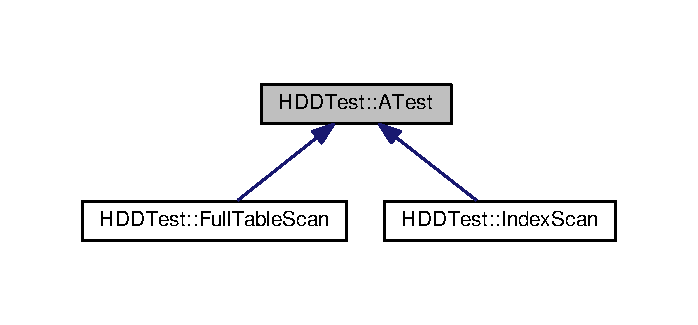
\includegraphics[width=335pt]{class_h_d_d_test_1_1_a_test__inherit__graph}
\end{center}
\end{figure}


Collaboration diagram for H\-D\-D\-Test\-:\-:A\-Test\-:\nopagebreak
\begin{figure}[H]
\begin{center}
\leavevmode
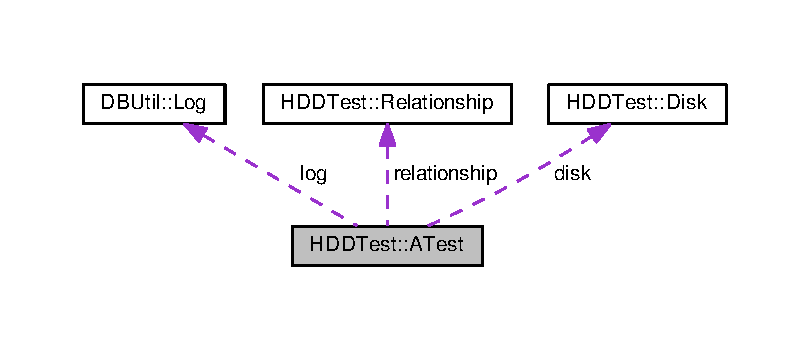
\includegraphics[width=350pt]{class_h_d_d_test_1_1_a_test__coll__graph}
\end{center}
\end{figure}
\subsection*{Public Member Functions}
\begin{DoxyCompactItemize}
\item 
\hyperlink{class_h_d_d_test_1_1_a_test_af07238e3cb280500d2c32968bd798b3b}{A\-Test} (std\-::string, \hyperlink{class_h_d_d_test_1_1_disk}{Disk} $\ast$, \hyperlink{class_h_d_d_test_1_1_relationship}{Relationship} $\ast$)
\item 
virtual \hyperlink{class_h_d_d_test_1_1_a_test_ac3b7b3b7fa2da5fa4c8b13bd95f46859}{$\sim$\-A\-Test} ()
\item 
void \hyperlink{class_h_d_d_test_1_1_a_test_a3c3ae1353dc05321bafa921ff6de4342}{start} ()
\item 
virtual void \hyperlink{class_h_d_d_test_1_1_a_test_a7dc054e211eccf42c03a6bb31d7fdc6e}{execute\-Test\-Algorithm} ()
\item 
void \hyperlink{class_h_d_d_test_1_1_a_test_a34afdf1fdbea73fd11422392eeb88320}{sleep} ()
\item 
void \hyperlink{class_h_d_d_test_1_1_a_test_ad4846b9edaba08c50795e0cb3f61c7cb}{start\-Background} ()
\end{DoxyCompactItemize}
\subsection*{Public Attributes}
\begin{DoxyCompactItemize}
\item 
std\-::string \hyperlink{class_h_d_d_test_1_1_a_test_aa7570476c8072fbbf8ec24c8f997656f}{name}
\item 
std\-::atomic$<$ bool $>$ \hyperlink{class_h_d_d_test_1_1_a_test_ac32f948a2541934bba8137e20987bf71}{is\-Main}
\item 
\hyperlink{class_d_b_util_1_1_log}{D\-B\-Util\-::\-Log} $\ast$ \hyperlink{class_h_d_d_test_1_1_a_test_a5db6314a0231c885e25a9c98ea41e95a}{log}
\end{DoxyCompactItemize}
\subsection*{Protected Attributes}
\begin{DoxyCompactItemize}
\item 
\hyperlink{class_h_d_d_test_1_1_relationship}{Relationship} $\ast$ \hyperlink{class_h_d_d_test_1_1_a_test_a2c3b0b7b9ec6c37f8dce5cceba4b728e}{relationship}
\item 
\hyperlink{class_h_d_d_test_1_1_disk}{Disk} $\ast$ \hyperlink{class_h_d_d_test_1_1_a_test_a8299c80c0778b70fabcc8af49e3f0334}{disk}
\item 
std\-::atomic$<$ bool $>$ \hyperlink{class_h_d_d_test_1_1_a_test_a3b5cdf4b9fef9a7c74ec02755a08df24}{runs}
\end{DoxyCompactItemize}


\subsection{Detailed Description}


Definition at line 27 of file A\-Test.\-h.



\subsection{Constructor \& Destructor Documentation}
\hypertarget{class_h_d_d_test_1_1_a_test_af07238e3cb280500d2c32968bd798b3b}{\index{H\-D\-D\-Test\-::\-A\-Test@{H\-D\-D\-Test\-::\-A\-Test}!A\-Test@{A\-Test}}
\index{A\-Test@{A\-Test}!HDDTest::ATest@{H\-D\-D\-Test\-::\-A\-Test}}
\subsubsection[{A\-Test}]{\setlength{\rightskip}{0pt plus 5cm}H\-D\-D\-Test\-::\-A\-Test\-::\-A\-Test (
\begin{DoxyParamCaption}
\item[{std\-::string}]{name, }
\item[{{\bf Disk} $\ast$}]{disk, }
\item[{{\bf Relationship} $\ast$}]{relationship}
\end{DoxyParamCaption}
)}}\label{class_h_d_d_test_1_1_a_test_af07238e3cb280500d2c32968bd798b3b}


Definition at line 13 of file A\-Test.\-cpp.

\hypertarget{class_h_d_d_test_1_1_a_test_ac3b7b3b7fa2da5fa4c8b13bd95f46859}{\index{H\-D\-D\-Test\-::\-A\-Test@{H\-D\-D\-Test\-::\-A\-Test}!$\sim$\-A\-Test@{$\sim$\-A\-Test}}
\index{$\sim$\-A\-Test@{$\sim$\-A\-Test}!HDDTest::ATest@{H\-D\-D\-Test\-::\-A\-Test}}
\subsubsection[{$\sim$\-A\-Test}]{\setlength{\rightskip}{0pt plus 5cm}H\-D\-D\-Test\-::\-A\-Test\-::$\sim$\-A\-Test (
\begin{DoxyParamCaption}
{}
\end{DoxyParamCaption}
)\hspace{0.3cm}{\ttfamily [virtual]}}}\label{class_h_d_d_test_1_1_a_test_ac3b7b3b7fa2da5fa4c8b13bd95f46859}


Definition at line 42 of file A\-Test.\-cpp.



\subsection{Member Function Documentation}
\hypertarget{class_h_d_d_test_1_1_a_test_a7dc054e211eccf42c03a6bb31d7fdc6e}{\index{H\-D\-D\-Test\-::\-A\-Test@{H\-D\-D\-Test\-::\-A\-Test}!execute\-Test\-Algorithm@{execute\-Test\-Algorithm}}
\index{execute\-Test\-Algorithm@{execute\-Test\-Algorithm}!HDDTest::ATest@{H\-D\-D\-Test\-::\-A\-Test}}
\subsubsection[{execute\-Test\-Algorithm}]{\setlength{\rightskip}{0pt plus 5cm}void H\-D\-D\-Test\-::\-A\-Test\-::execute\-Test\-Algorithm (
\begin{DoxyParamCaption}
{}
\end{DoxyParamCaption}
)\hspace{0.3cm}{\ttfamily [virtual]}}}\label{class_h_d_d_test_1_1_a_test_a7dc054e211eccf42c03a6bb31d7fdc6e}


Reimplemented in \hyperlink{class_h_d_d_test_1_1_full_table_scan_a732473e7440538517ab2c1f6e9e636eb}{H\-D\-D\-Test\-::\-Full\-Table\-Scan}, and \hyperlink{class_h_d_d_test_1_1_index_scan_a63c295ffb3dd74515cf6c6583c9dc462}{H\-D\-D\-Test\-::\-Index\-Scan}.



Definition at line 40 of file A\-Test.\-cpp.



Here is the caller graph for this function\-:\nopagebreak
\begin{figure}[H]
\begin{center}
\leavevmode
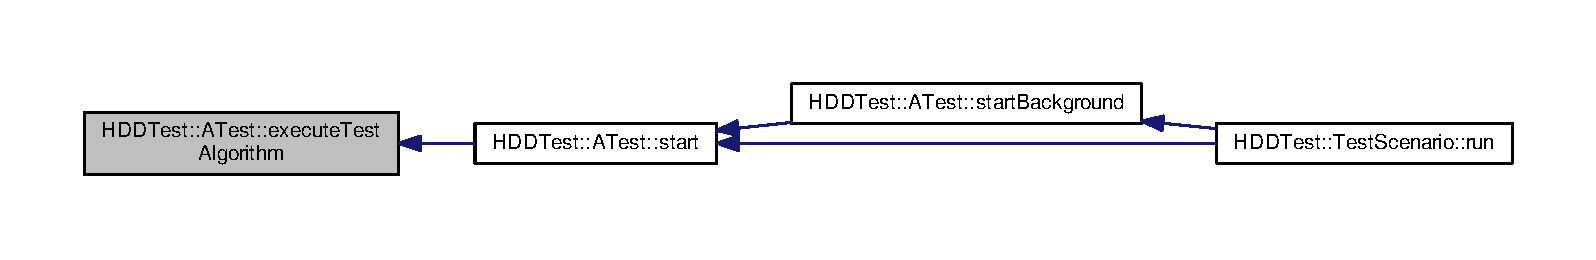
\includegraphics[width=350pt]{class_h_d_d_test_1_1_a_test_a7dc054e211eccf42c03a6bb31d7fdc6e_icgraph}
\end{center}
\end{figure}


\hypertarget{class_h_d_d_test_1_1_a_test_a34afdf1fdbea73fd11422392eeb88320}{\index{H\-D\-D\-Test\-::\-A\-Test@{H\-D\-D\-Test\-::\-A\-Test}!sleep@{sleep}}
\index{sleep@{sleep}!HDDTest::ATest@{H\-D\-D\-Test\-::\-A\-Test}}
\subsubsection[{sleep}]{\setlength{\rightskip}{0pt plus 5cm}void H\-D\-D\-Test\-::\-A\-Test\-::sleep (
\begin{DoxyParamCaption}
{}
\end{DoxyParamCaption}
)}}\label{class_h_d_d_test_1_1_a_test_a34afdf1fdbea73fd11422392eeb88320}


Definition at line 47 of file A\-Test.\-cpp.



Here is the caller graph for this function\-:\nopagebreak
\begin{figure}[H]
\begin{center}
\leavevmode
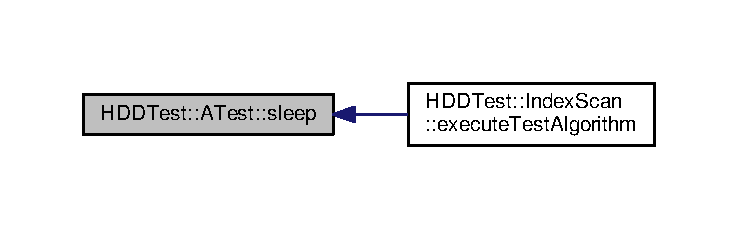
\includegraphics[width=350pt]{class_h_d_d_test_1_1_a_test_a34afdf1fdbea73fd11422392eeb88320_icgraph}
\end{center}
\end{figure}


\hypertarget{class_h_d_d_test_1_1_a_test_a3c3ae1353dc05321bafa921ff6de4342}{\index{H\-D\-D\-Test\-::\-A\-Test@{H\-D\-D\-Test\-::\-A\-Test}!start@{start}}
\index{start@{start}!HDDTest::ATest@{H\-D\-D\-Test\-::\-A\-Test}}
\subsubsection[{start}]{\setlength{\rightskip}{0pt plus 5cm}void H\-D\-D\-Test\-::\-A\-Test\-::start (
\begin{DoxyParamCaption}
{}
\end{DoxyParamCaption}
)}}\label{class_h_d_d_test_1_1_a_test_a3c3ae1353dc05321bafa921ff6de4342}


Definition at line 23 of file A\-Test.\-cpp.



Here is the call graph for this function\-:\nopagebreak
\begin{figure}[H]
\begin{center}
\leavevmode
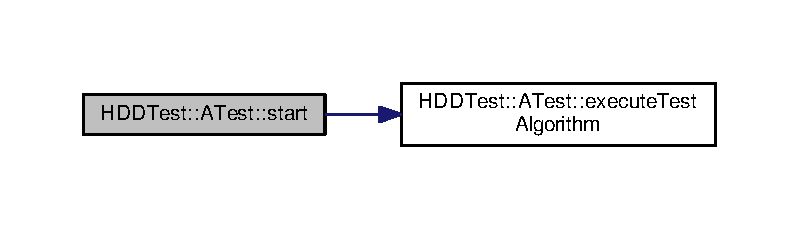
\includegraphics[width=350pt]{class_h_d_d_test_1_1_a_test_a3c3ae1353dc05321bafa921ff6de4342_cgraph}
\end{center}
\end{figure}




Here is the caller graph for this function\-:\nopagebreak
\begin{figure}[H]
\begin{center}
\leavevmode
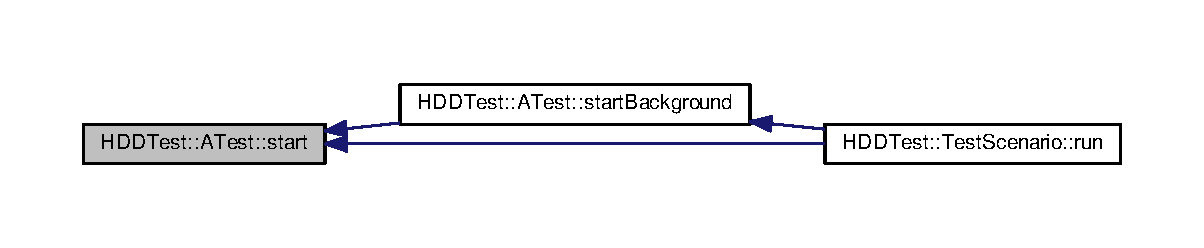
\includegraphics[width=350pt]{class_h_d_d_test_1_1_a_test_a3c3ae1353dc05321bafa921ff6de4342_icgraph}
\end{center}
\end{figure}


\hypertarget{class_h_d_d_test_1_1_a_test_ad4846b9edaba08c50795e0cb3f61c7cb}{\index{H\-D\-D\-Test\-::\-A\-Test@{H\-D\-D\-Test\-::\-A\-Test}!start\-Background@{start\-Background}}
\index{start\-Background@{start\-Background}!HDDTest::ATest@{H\-D\-D\-Test\-::\-A\-Test}}
\subsubsection[{start\-Background}]{\setlength{\rightskip}{0pt plus 5cm}void H\-D\-D\-Test\-::\-A\-Test\-::start\-Background (
\begin{DoxyParamCaption}
{}
\end{DoxyParamCaption}
)}}\label{class_h_d_d_test_1_1_a_test_ad4846b9edaba08c50795e0cb3f61c7cb}


Definition at line 51 of file A\-Test.\-cpp.



Here is the call graph for this function\-:\nopagebreak
\begin{figure}[H]
\begin{center}
\leavevmode
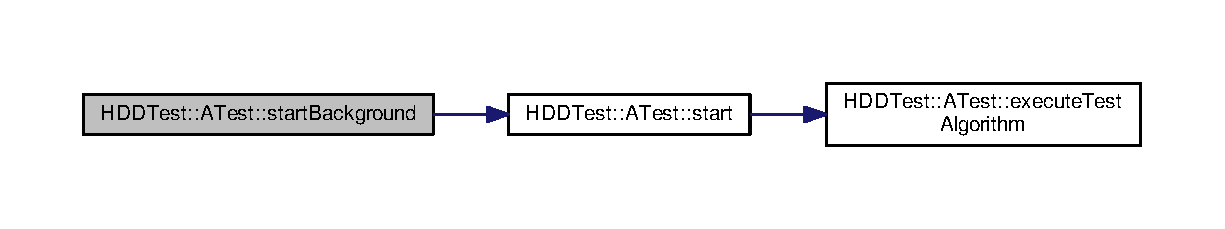
\includegraphics[width=350pt]{class_h_d_d_test_1_1_a_test_ad4846b9edaba08c50795e0cb3f61c7cb_cgraph}
\end{center}
\end{figure}




Here is the caller graph for this function\-:\nopagebreak
\begin{figure}[H]
\begin{center}
\leavevmode
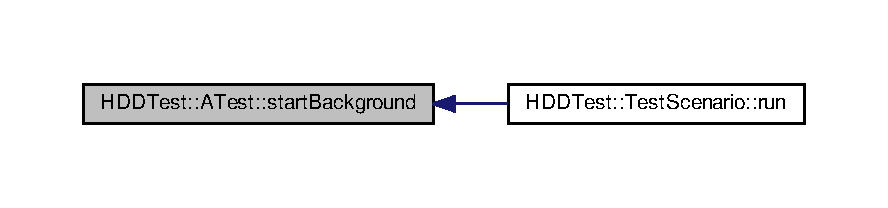
\includegraphics[width=350pt]{class_h_d_d_test_1_1_a_test_ad4846b9edaba08c50795e0cb3f61c7cb_icgraph}
\end{center}
\end{figure}




\subsection{Member Data Documentation}
\hypertarget{class_h_d_d_test_1_1_a_test_a8299c80c0778b70fabcc8af49e3f0334}{\index{H\-D\-D\-Test\-::\-A\-Test@{H\-D\-D\-Test\-::\-A\-Test}!disk@{disk}}
\index{disk@{disk}!HDDTest::ATest@{H\-D\-D\-Test\-::\-A\-Test}}
\subsubsection[{disk}]{\setlength{\rightskip}{0pt plus 5cm}{\bf Disk}$\ast$ H\-D\-D\-Test\-::\-A\-Test\-::disk\hspace{0.3cm}{\ttfamily [protected]}}}\label{class_h_d_d_test_1_1_a_test_a8299c80c0778b70fabcc8af49e3f0334}


Definition at line 42 of file A\-Test.\-h.

\hypertarget{class_h_d_d_test_1_1_a_test_ac32f948a2541934bba8137e20987bf71}{\index{H\-D\-D\-Test\-::\-A\-Test@{H\-D\-D\-Test\-::\-A\-Test}!is\-Main@{is\-Main}}
\index{is\-Main@{is\-Main}!HDDTest::ATest@{H\-D\-D\-Test\-::\-A\-Test}}
\subsubsection[{is\-Main}]{\setlength{\rightskip}{0pt plus 5cm}std\-::atomic$<$bool$>$ H\-D\-D\-Test\-::\-A\-Test\-::is\-Main}}\label{class_h_d_d_test_1_1_a_test_ac32f948a2541934bba8137e20987bf71}


Definition at line 31 of file A\-Test.\-h.

\hypertarget{class_h_d_d_test_1_1_a_test_a5db6314a0231c885e25a9c98ea41e95a}{\index{H\-D\-D\-Test\-::\-A\-Test@{H\-D\-D\-Test\-::\-A\-Test}!log@{log}}
\index{log@{log}!HDDTest::ATest@{H\-D\-D\-Test\-::\-A\-Test}}
\subsubsection[{log}]{\setlength{\rightskip}{0pt plus 5cm}{\bf D\-B\-Util\-::\-Log}$\ast$ H\-D\-D\-Test\-::\-A\-Test\-::log}}\label{class_h_d_d_test_1_1_a_test_a5db6314a0231c885e25a9c98ea41e95a}


Definition at line 38 of file A\-Test.\-h.

\hypertarget{class_h_d_d_test_1_1_a_test_aa7570476c8072fbbf8ec24c8f997656f}{\index{H\-D\-D\-Test\-::\-A\-Test@{H\-D\-D\-Test\-::\-A\-Test}!name@{name}}
\index{name@{name}!HDDTest::ATest@{H\-D\-D\-Test\-::\-A\-Test}}
\subsubsection[{name}]{\setlength{\rightskip}{0pt plus 5cm}std\-::string H\-D\-D\-Test\-::\-A\-Test\-::name}}\label{class_h_d_d_test_1_1_a_test_aa7570476c8072fbbf8ec24c8f997656f}


Definition at line 30 of file A\-Test.\-h.

\hypertarget{class_h_d_d_test_1_1_a_test_a2c3b0b7b9ec6c37f8dce5cceba4b728e}{\index{H\-D\-D\-Test\-::\-A\-Test@{H\-D\-D\-Test\-::\-A\-Test}!relationship@{relationship}}
\index{relationship@{relationship}!HDDTest::ATest@{H\-D\-D\-Test\-::\-A\-Test}}
\subsubsection[{relationship}]{\setlength{\rightskip}{0pt plus 5cm}{\bf Relationship}$\ast$ H\-D\-D\-Test\-::\-A\-Test\-::relationship\hspace{0.3cm}{\ttfamily [protected]}}}\label{class_h_d_d_test_1_1_a_test_a2c3b0b7b9ec6c37f8dce5cceba4b728e}


Definition at line 41 of file A\-Test.\-h.

\hypertarget{class_h_d_d_test_1_1_a_test_a3b5cdf4b9fef9a7c74ec02755a08df24}{\index{H\-D\-D\-Test\-::\-A\-Test@{H\-D\-D\-Test\-::\-A\-Test}!runs@{runs}}
\index{runs@{runs}!HDDTest::ATest@{H\-D\-D\-Test\-::\-A\-Test}}
\subsubsection[{runs}]{\setlength{\rightskip}{0pt plus 5cm}std\-::atomic$<$bool$>$ H\-D\-D\-Test\-::\-A\-Test\-::runs\hspace{0.3cm}{\ttfamily [protected]}}}\label{class_h_d_d_test_1_1_a_test_a3b5cdf4b9fef9a7c74ec02755a08df24}


Definition at line 43 of file A\-Test.\-h.



The documentation for this class was generated from the following files\-:\begin{DoxyCompactItemize}
\item 
src/\-Tests/\hyperlink{_a_test_8h}{A\-Test.\-h}\item 
src/\-Tests/\hyperlink{_a_test_8cpp}{A\-Test.\-cpp}\end{DoxyCompactItemize}

\hypertarget{class_h_d_d_test_1_1_configurator}{\section{H\-D\-D\-Test\-:\-:Configurator Class Reference}
\label{class_h_d_d_test_1_1_configurator}\index{H\-D\-D\-Test\-::\-Configurator@{H\-D\-D\-Test\-::\-Configurator}}
}


{\ttfamily \#include $<$Configurator.\-h$>$}

\subsection*{Public Member Functions}
\begin{DoxyCompactItemize}
\item 
\hyperlink{class_h_d_d_test_1_1_configurator_a33abd9be7ab39d0dc567d8f86c7b463e}{Configurator} ()
\item 
virtual \hyperlink{class_h_d_d_test_1_1_configurator_ace450749321fcdc845940c5686d280a7}{$\sim$\-Configurator} ()
\item 
std\-::vector$<$ \hyperlink{class_h_d_d_test_1_1_test_scenario}{Test\-Scenario} $\ast$ $>$ $\ast$ \hyperlink{class_h_d_d_test_1_1_configurator_a77eb045da43a5c8ffde204f8e86e9e9e}{get\-Test\-Scenarios} ()
\end{DoxyCompactItemize}


\subsection{Detailed Description}


Definition at line 24 of file Configurator.\-h.



\subsection{Constructor \& Destructor Documentation}
\hypertarget{class_h_d_d_test_1_1_configurator_a33abd9be7ab39d0dc567d8f86c7b463e}{\index{H\-D\-D\-Test\-::\-Configurator@{H\-D\-D\-Test\-::\-Configurator}!Configurator@{Configurator}}
\index{Configurator@{Configurator}!HDDTest::Configurator@{H\-D\-D\-Test\-::\-Configurator}}
\subsubsection[{Configurator}]{\setlength{\rightskip}{0pt plus 5cm}H\-D\-D\-Test\-::\-Configurator\-::\-Configurator (
\begin{DoxyParamCaption}
{}
\end{DoxyParamCaption}
)}}\label{class_h_d_d_test_1_1_configurator_a33abd9be7ab39d0dc567d8f86c7b463e}


Definition at line 14 of file Configurator.\-cpp.

\hypertarget{class_h_d_d_test_1_1_configurator_ace450749321fcdc845940c5686d280a7}{\index{H\-D\-D\-Test\-::\-Configurator@{H\-D\-D\-Test\-::\-Configurator}!$\sim$\-Configurator@{$\sim$\-Configurator}}
\index{$\sim$\-Configurator@{$\sim$\-Configurator}!HDDTest::Configurator@{H\-D\-D\-Test\-::\-Configurator}}
\subsubsection[{$\sim$\-Configurator}]{\setlength{\rightskip}{0pt plus 5cm}H\-D\-D\-Test\-::\-Configurator\-::$\sim$\-Configurator (
\begin{DoxyParamCaption}
{}
\end{DoxyParamCaption}
)\hspace{0.3cm}{\ttfamily [virtual]}}}\label{class_h_d_d_test_1_1_configurator_ace450749321fcdc845940c5686d280a7}


Definition at line 20 of file Configurator.\-cpp.



\subsection{Member Function Documentation}
\hypertarget{class_h_d_d_test_1_1_configurator_a77eb045da43a5c8ffde204f8e86e9e9e}{\index{H\-D\-D\-Test\-::\-Configurator@{H\-D\-D\-Test\-::\-Configurator}!get\-Test\-Scenarios@{get\-Test\-Scenarios}}
\index{get\-Test\-Scenarios@{get\-Test\-Scenarios}!HDDTest::Configurator@{H\-D\-D\-Test\-::\-Configurator}}
\subsubsection[{get\-Test\-Scenarios}]{\setlength{\rightskip}{0pt plus 5cm}std\-::vector$<$ {\bf Test\-Scenario} $\ast$ $>$ $\ast$ H\-D\-D\-Test\-::\-Configurator\-::get\-Test\-Scenarios (
\begin{DoxyParamCaption}
{}
\end{DoxyParamCaption}
)}}\label{class_h_d_d_test_1_1_configurator_a77eb045da43a5c8ffde204f8e86e9e9e}


Definition at line 32 of file Configurator.\-cpp.



Here is the caller graph for this function\-:
\nopagebreak
\begin{figure}[H]
\begin{center}
\leavevmode
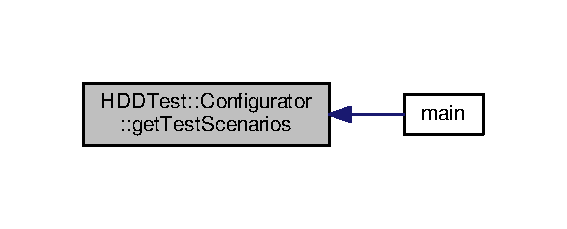
\includegraphics[width=272pt]{class_h_d_d_test_1_1_configurator_a77eb045da43a5c8ffde204f8e86e9e9e_icgraph}
\end{center}
\end{figure}




The documentation for this class was generated from the following files\-:\begin{DoxyCompactItemize}
\item 
src/\-Util/\hyperlink{_configurator_8h}{Configurator.\-h}\item 
src/\-Util/\hyperlink{_configurator_8cpp}{Configurator.\-cpp}\end{DoxyCompactItemize}

\hypertarget{class_h_d_d_test_1_1_disk}{\section{H\-D\-D\-Test\-:\-:Disk Class Reference}
\label{class_h_d_d_test_1_1_disk}\index{H\-D\-D\-Test\-::\-Disk@{H\-D\-D\-Test\-::\-Disk}}
}


{\ttfamily \#include $<$Disk.\-h$>$}

\subsection*{Public Member Functions}
\begin{DoxyCompactItemize}
\item 
void \hyperlink{class_h_d_d_test_1_1_disk_a5afff4786de776408acd86e3a91206c7}{read\-Page} (uint64\-\_\-t)
\item 
void \hyperlink{class_h_d_d_test_1_1_disk_adb3541b1531a7029e5d688f123df9baf}{read\-Extent} (uint64\-\_\-t)
\item 
void \hyperlink{class_h_d_d_test_1_1_disk_a538c61b9ff956231d7f05d19419eada1}{write\-Page} (uint64\-\_\-t)
\item 
void \hyperlink{class_h_d_d_test_1_1_disk_a4954ba9185b24bb98828934cb116b8dd}{write\-Extent} (uint64\-\_\-t)
\item 
void \hyperlink{class_h_d_d_test_1_1_disk_a08131fbb8f001b5f8b60056308f5a8da}{del} ()
\item 
void \hyperlink{class_h_d_d_test_1_1_disk_a161bd5f5921eb78bdd7a51757267e61b}{set\-Page\-Size} (int)
\begin{DoxyCompactList}\small\item\em \mbox{[}brief description\mbox{]} \end{DoxyCompactList}\item 
void \hyperlink{class_h_d_d_test_1_1_disk_a78e515afa9536ed390d317c1f595fe9e}{set\-Extent\-Size} (int)
\begin{DoxyCompactList}\small\item\em extent-\/size-\/setter \end{DoxyCompactList}\end{DoxyCompactItemize}
\subsection*{Static Public Member Functions}
\begin{DoxyCompactItemize}
\item 
static \hyperlink{class_h_d_d_test_1_1_disk}{Disk} $\ast$ \hyperlink{class_h_d_d_test_1_1_disk_a0f6006970c964527bb5a2e6e0cb16b87}{get} (std\-::string)
\begin{DoxyCompactList}\small\item\em returns disk \end{DoxyCompactList}\end{DoxyCompactItemize}
\subsection*{Public Attributes}
\begin{DoxyCompactItemize}
\item 
std\-::string \hyperlink{class_h_d_d_test_1_1_disk_ac8e5dd8530a2f2913a8d1f25013549a4}{path}
\end{DoxyCompactItemize}
\subsection*{Protected Member Functions}
\begin{DoxyCompactItemize}
\item 
bool \hyperlink{class_h_d_d_test_1_1_disk_a94248b3946f474cce092b5768cfaf8fd}{is\-Valid} ()
\end{DoxyCompactItemize}


\subsection{Detailed Description}


Definition at line 19 of file Disk.\-h.



\subsection{Member Function Documentation}
\hypertarget{class_h_d_d_test_1_1_disk_a08131fbb8f001b5f8b60056308f5a8da}{\index{H\-D\-D\-Test\-::\-Disk@{H\-D\-D\-Test\-::\-Disk}!del@{del}}
\index{del@{del}!HDDTest::Disk@{H\-D\-D\-Test\-::\-Disk}}
\subsubsection[{del}]{\setlength{\rightskip}{0pt plus 5cm}void H\-D\-D\-Test\-::\-Disk\-::del (
\begin{DoxyParamCaption}
{}
\end{DoxyParamCaption}
)}}\label{class_h_d_d_test_1_1_disk_a08131fbb8f001b5f8b60056308f5a8da}


Definition at line 124 of file Disk.\-cpp.

\hypertarget{class_h_d_d_test_1_1_disk_a0f6006970c964527bb5a2e6e0cb16b87}{\index{H\-D\-D\-Test\-::\-Disk@{H\-D\-D\-Test\-::\-Disk}!get@{get}}
\index{get@{get}!HDDTest::Disk@{H\-D\-D\-Test\-::\-Disk}}
\subsubsection[{get}]{\setlength{\rightskip}{0pt plus 5cm}{\bf Disk} $\ast$ H\-D\-D\-Test\-::\-Disk\-::get (
\begin{DoxyParamCaption}
\item[{std\-::string}]{path}
\end{DoxyParamCaption}
)\hspace{0.3cm}{\ttfamily [static]}}}\label{class_h_d_d_test_1_1_disk_a0f6006970c964527bb5a2e6e0cb16b87}


returns disk 

returns a disk pointer


\begin{DoxyParams}{Parameters}
{\em path} & disk path \\
\hline
\end{DoxyParams}
\begin{DoxyReturn}{Returns}
pointer to disk instance 
\end{DoxyReturn}


Definition at line 20 of file Disk.\-cpp.



Here is the caller graph for this function\-:
\nopagebreak
\begin{figure}[H]
\begin{center}
\leavevmode
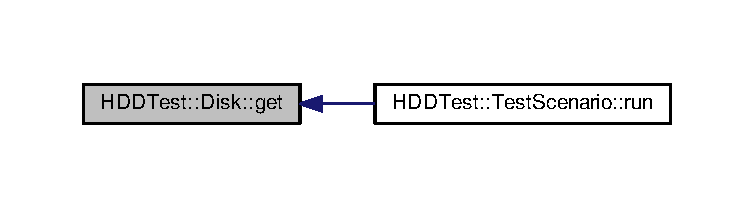
\includegraphics[width=350pt]{class_h_d_d_test_1_1_disk_a0f6006970c964527bb5a2e6e0cb16b87_icgraph}
\end{center}
\end{figure}


\hypertarget{class_h_d_d_test_1_1_disk_a94248b3946f474cce092b5768cfaf8fd}{\index{H\-D\-D\-Test\-::\-Disk@{H\-D\-D\-Test\-::\-Disk}!is\-Valid@{is\-Valid}}
\index{is\-Valid@{is\-Valid}!HDDTest::Disk@{H\-D\-D\-Test\-::\-Disk}}
\subsubsection[{is\-Valid}]{\setlength{\rightskip}{0pt plus 5cm}bool H\-D\-D\-Test\-::\-Disk\-::is\-Valid (
\begin{DoxyParamCaption}
{}
\end{DoxyParamCaption}
)\hspace{0.3cm}{\ttfamily [protected]}}}\label{class_h_d_d_test_1_1_disk_a94248b3946f474cce092b5768cfaf8fd}


Definition at line 130 of file Disk.\-cpp.

\hypertarget{class_h_d_d_test_1_1_disk_adb3541b1531a7029e5d688f123df9baf}{\index{H\-D\-D\-Test\-::\-Disk@{H\-D\-D\-Test\-::\-Disk}!read\-Extent@{read\-Extent}}
\index{read\-Extent@{read\-Extent}!HDDTest::Disk@{H\-D\-D\-Test\-::\-Disk}}
\subsubsection[{read\-Extent}]{\setlength{\rightskip}{0pt plus 5cm}void H\-D\-D\-Test\-::\-Disk\-::read\-Extent (
\begin{DoxyParamCaption}
\item[{uint64\-\_\-t}]{start}
\end{DoxyParamCaption}
)}}\label{class_h_d_d_test_1_1_disk_adb3541b1531a7029e5d688f123df9baf}


Definition at line 97 of file Disk.\-cpp.



Here is the caller graph for this function\-:
\nopagebreak
\begin{figure}[H]
\begin{center}
\leavevmode
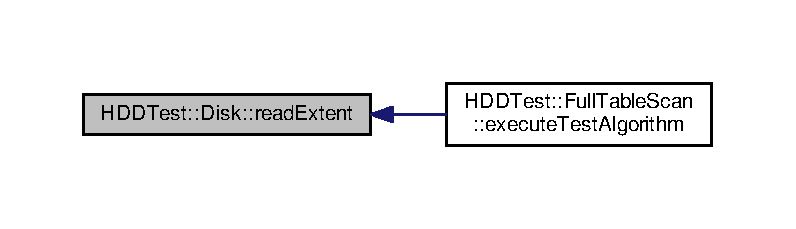
\includegraphics[width=350pt]{class_h_d_d_test_1_1_disk_adb3541b1531a7029e5d688f123df9baf_icgraph}
\end{center}
\end{figure}


\hypertarget{class_h_d_d_test_1_1_disk_a5afff4786de776408acd86e3a91206c7}{\index{H\-D\-D\-Test\-::\-Disk@{H\-D\-D\-Test\-::\-Disk}!read\-Page@{read\-Page}}
\index{read\-Page@{read\-Page}!HDDTest::Disk@{H\-D\-D\-Test\-::\-Disk}}
\subsubsection[{read\-Page}]{\setlength{\rightskip}{0pt plus 5cm}void H\-D\-D\-Test\-::\-Disk\-::read\-Page (
\begin{DoxyParamCaption}
\item[{uint64\-\_\-t}]{start}
\end{DoxyParamCaption}
)}}\label{class_h_d_d_test_1_1_disk_a5afff4786de776408acd86e3a91206c7}


Definition at line 103 of file Disk.\-cpp.



Here is the caller graph for this function\-:
\nopagebreak
\begin{figure}[H]
\begin{center}
\leavevmode
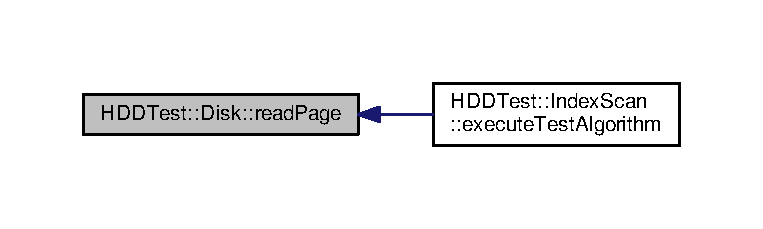
\includegraphics[width=350pt]{class_h_d_d_test_1_1_disk_a5afff4786de776408acd86e3a91206c7_icgraph}
\end{center}
\end{figure}


\hypertarget{class_h_d_d_test_1_1_disk_a78e515afa9536ed390d317c1f595fe9e}{\index{H\-D\-D\-Test\-::\-Disk@{H\-D\-D\-Test\-::\-Disk}!set\-Extent\-Size@{set\-Extent\-Size}}
\index{set\-Extent\-Size@{set\-Extent\-Size}!HDDTest::Disk@{H\-D\-D\-Test\-::\-Disk}}
\subsubsection[{set\-Extent\-Size}]{\setlength{\rightskip}{0pt plus 5cm}void H\-D\-D\-Test\-::\-Disk\-::set\-Extent\-Size (
\begin{DoxyParamCaption}
\item[{int}]{size}
\end{DoxyParamCaption}
)}}\label{class_h_d_d_test_1_1_disk_a78e515afa9536ed390d317c1f595fe9e}


extent-\/size-\/setter 

sets the extent size in kb


\begin{DoxyParams}{Parameters}
{\em size} & Size of a extent in kb \\
\hline
\end{DoxyParams}


Definition at line 78 of file Disk.\-cpp.

\hypertarget{class_h_d_d_test_1_1_disk_a161bd5f5921eb78bdd7a51757267e61b}{\index{H\-D\-D\-Test\-::\-Disk@{H\-D\-D\-Test\-::\-Disk}!set\-Page\-Size@{set\-Page\-Size}}
\index{set\-Page\-Size@{set\-Page\-Size}!HDDTest::Disk@{H\-D\-D\-Test\-::\-Disk}}
\subsubsection[{set\-Page\-Size}]{\setlength{\rightskip}{0pt plus 5cm}void H\-D\-D\-Test\-::\-Disk\-::set\-Page\-Size (
\begin{DoxyParamCaption}
\item[{int}]{size}
\end{DoxyParamCaption}
)}}\label{class_h_d_d_test_1_1_disk_a161bd5f5921eb78bdd7a51757267e61b}


\mbox{[}brief description\mbox{]} 

\mbox{[}long description\mbox{]}


\begin{DoxyParams}{Parameters}
{\em size} & \mbox{[}description\mbox{]} \\
\hline
\end{DoxyParams}


Definition at line 90 of file Disk.\-cpp.

\hypertarget{class_h_d_d_test_1_1_disk_a4954ba9185b24bb98828934cb116b8dd}{\index{H\-D\-D\-Test\-::\-Disk@{H\-D\-D\-Test\-::\-Disk}!write\-Extent@{write\-Extent}}
\index{write\-Extent@{write\-Extent}!HDDTest::Disk@{H\-D\-D\-Test\-::\-Disk}}
\subsubsection[{write\-Extent}]{\setlength{\rightskip}{0pt plus 5cm}void H\-D\-D\-Test\-::\-Disk\-::write\-Extent (
\begin{DoxyParamCaption}
\item[{uint64\-\_\-t}]{start}
\end{DoxyParamCaption}
)}}\label{class_h_d_d_test_1_1_disk_a4954ba9185b24bb98828934cb116b8dd}


Definition at line 111 of file Disk.\-cpp.

\hypertarget{class_h_d_d_test_1_1_disk_a538c61b9ff956231d7f05d19419eada1}{\index{H\-D\-D\-Test\-::\-Disk@{H\-D\-D\-Test\-::\-Disk}!write\-Page@{write\-Page}}
\index{write\-Page@{write\-Page}!HDDTest::Disk@{H\-D\-D\-Test\-::\-Disk}}
\subsubsection[{write\-Page}]{\setlength{\rightskip}{0pt plus 5cm}void H\-D\-D\-Test\-::\-Disk\-::write\-Page (
\begin{DoxyParamCaption}
\item[{uint64\-\_\-t}]{start}
\end{DoxyParamCaption}
)}}\label{class_h_d_d_test_1_1_disk_a538c61b9ff956231d7f05d19419eada1}


Definition at line 117 of file Disk.\-cpp.



\subsection{Member Data Documentation}
\hypertarget{class_h_d_d_test_1_1_disk_ac8e5dd8530a2f2913a8d1f25013549a4}{\index{H\-D\-D\-Test\-::\-Disk@{H\-D\-D\-Test\-::\-Disk}!path@{path}}
\index{path@{path}!HDDTest::Disk@{H\-D\-D\-Test\-::\-Disk}}
\subsubsection[{path}]{\setlength{\rightskip}{0pt plus 5cm}std\-::string H\-D\-D\-Test\-::\-Disk\-::path}}\label{class_h_d_d_test_1_1_disk_ac8e5dd8530a2f2913a8d1f25013549a4}


Definition at line 34 of file Disk.\-h.



The documentation for this class was generated from the following files\-:\begin{DoxyCompactItemize}
\item 
src/\-Util/\hyperlink{_disk_8h}{Disk.\-h}\item 
src/\-Util/\hyperlink{_disk_8cpp}{Disk.\-cpp}\end{DoxyCompactItemize}

\hypertarget{struct_h_d_d_test_1_1_extent}{\section{H\-D\-D\-Test\-:\-:Extent Struct Reference}
\label{struct_h_d_d_test_1_1_extent}\index{H\-D\-D\-Test\-::\-Extent@{H\-D\-D\-Test\-::\-Extent}}
}


{\ttfamily \#include $<$Relationship.\-h$>$}

\subsection*{Public Attributes}
\begin{DoxyCompactItemize}
\item 
unsigned long long int \hyperlink{struct_h_d_d_test_1_1_extent_ac636e4602549d5881611e51b7f10eefd}{number}
\item 
unsigned long long int \hyperlink{struct_h_d_d_test_1_1_extent_aee160e4b0ea953d7164fb41d6a69206c}{start\-Kb}
\end{DoxyCompactItemize}


\subsection{Detailed Description}


Definition at line 15 of file Relationship.\-h.



\subsection{Member Data Documentation}
\hypertarget{struct_h_d_d_test_1_1_extent_ac636e4602549d5881611e51b7f10eefd}{\index{H\-D\-D\-Test\-::\-Extent@{H\-D\-D\-Test\-::\-Extent}!number@{number}}
\index{number@{number}!HDDTest::Extent@{H\-D\-D\-Test\-::\-Extent}}
\subsubsection[{number}]{\setlength{\rightskip}{0pt plus 5cm}unsigned long long int H\-D\-D\-Test\-::\-Extent\-::number}}\label{struct_h_d_d_test_1_1_extent_ac636e4602549d5881611e51b7f10eefd}


Definition at line 17 of file Relationship.\-h.

\hypertarget{struct_h_d_d_test_1_1_extent_aee160e4b0ea953d7164fb41d6a69206c}{\index{H\-D\-D\-Test\-::\-Extent@{H\-D\-D\-Test\-::\-Extent}!start\-Kb@{start\-Kb}}
\index{start\-Kb@{start\-Kb}!HDDTest::Extent@{H\-D\-D\-Test\-::\-Extent}}
\subsubsection[{start\-Kb}]{\setlength{\rightskip}{0pt plus 5cm}unsigned long long int H\-D\-D\-Test\-::\-Extent\-::start\-Kb}}\label{struct_h_d_d_test_1_1_extent_aee160e4b0ea953d7164fb41d6a69206c}


Definition at line 18 of file Relationship.\-h.



The documentation for this struct was generated from the following file\-:\begin{DoxyCompactItemize}
\item 
src/\-Layout/\hyperlink{_relationship_8h}{Relationship.\-h}\end{DoxyCompactItemize}

\hypertarget{class_h_d_d_test_1_1_full_table_scan}{\section{H\-D\-D\-Test\-:\-:Full\-Table\-Scan Class Reference}
\label{class_h_d_d_test_1_1_full_table_scan}\index{H\-D\-D\-Test\-::\-Full\-Table\-Scan@{H\-D\-D\-Test\-::\-Full\-Table\-Scan}}
}


Inheritance diagram for H\-D\-D\-Test\-:\-:Full\-Table\-Scan\-:
\nopagebreak
\begin{figure}[H]
\begin{center}
\leavevmode
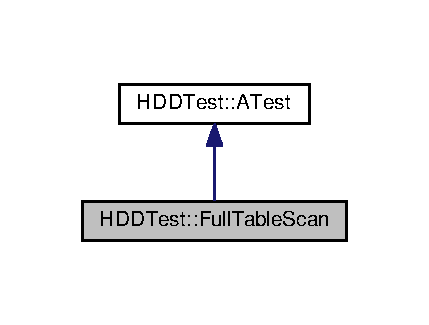
\includegraphics[width=206pt]{class_h_d_d_test_1_1_full_table_scan__inherit__graph}
\end{center}
\end{figure}


Collaboration diagram for H\-D\-D\-Test\-:\-:Full\-Table\-Scan\-:
\nopagebreak
\begin{figure}[H]
\begin{center}
\leavevmode
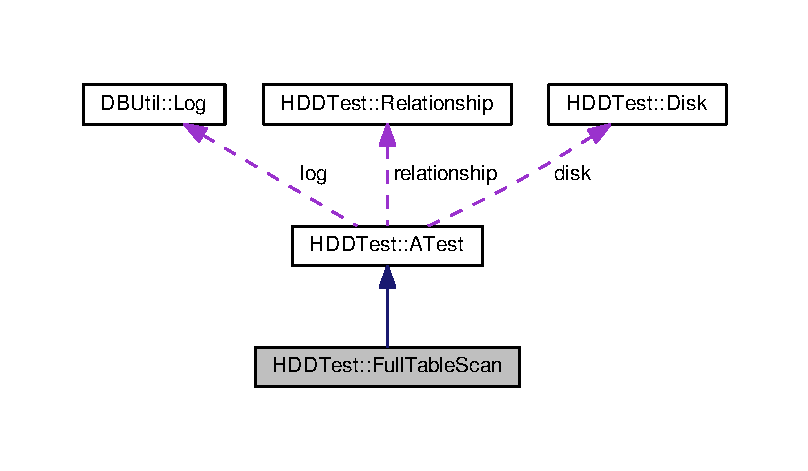
\includegraphics[width=350pt]{class_h_d_d_test_1_1_full_table_scan__coll__graph}
\end{center}
\end{figure}
\subsection*{Public Member Functions}
\begin{DoxyCompactItemize}
\item 
\hyperlink{class_h_d_d_test_1_1_full_table_scan_a7c4efb4b22a6d61f9ae672fcf64b147e}{Full\-Table\-Scan} (std\-::string, \hyperlink{class_h_d_d_test_1_1_disk}{Disk} $\ast$, \hyperlink{class_h_d_d_test_1_1_relationship}{Relationship} $\ast$)
\item 
virtual \hyperlink{class_h_d_d_test_1_1_full_table_scan_aeea7425b20a671f3fd55fca6a2a3620d}{$\sim$\-Full\-Table\-Scan} ()
\item 
void \hyperlink{class_h_d_d_test_1_1_full_table_scan_a732473e7440538517ab2c1f6e9e636eb}{execute\-Test\-Algorithm} () override
\end{DoxyCompactItemize}
\subsection*{Additional Inherited Members}


\subsection{Detailed Description}


Definition at line 16 of file Full\-Table\-Scan.\-cpp.



\subsection{Constructor \& Destructor Documentation}
\hypertarget{class_h_d_d_test_1_1_full_table_scan_a7c4efb4b22a6d61f9ae672fcf64b147e}{\index{H\-D\-D\-Test\-::\-Full\-Table\-Scan@{H\-D\-D\-Test\-::\-Full\-Table\-Scan}!Full\-Table\-Scan@{Full\-Table\-Scan}}
\index{Full\-Table\-Scan@{Full\-Table\-Scan}!HDDTest::FullTableScan@{H\-D\-D\-Test\-::\-Full\-Table\-Scan}}
\subsubsection[{Full\-Table\-Scan}]{\setlength{\rightskip}{0pt plus 5cm}H\-D\-D\-Test\-::\-Full\-Table\-Scan\-::\-Full\-Table\-Scan (
\begin{DoxyParamCaption}
\item[{std\-::string}]{name, }
\item[{{\bf Disk} $\ast$}]{disk, }
\item[{{\bf Relationship} $\ast$}]{relationship}
\end{DoxyParamCaption}
)}}\label{class_h_d_d_test_1_1_full_table_scan_a7c4efb4b22a6d61f9ae672fcf64b147e}


Definition at line 13 of file Full\-Table\-Scan.\-h.

\hypertarget{class_h_d_d_test_1_1_full_table_scan_aeea7425b20a671f3fd55fca6a2a3620d}{\index{H\-D\-D\-Test\-::\-Full\-Table\-Scan@{H\-D\-D\-Test\-::\-Full\-Table\-Scan}!$\sim$\-Full\-Table\-Scan@{$\sim$\-Full\-Table\-Scan}}
\index{$\sim$\-Full\-Table\-Scan@{$\sim$\-Full\-Table\-Scan}!HDDTest::FullTableScan@{H\-D\-D\-Test\-::\-Full\-Table\-Scan}}
\subsubsection[{$\sim$\-Full\-Table\-Scan}]{\setlength{\rightskip}{0pt plus 5cm}H\-D\-D\-Test\-::\-Full\-Table\-Scan\-::$\sim$\-Full\-Table\-Scan (
\begin{DoxyParamCaption}
{}
\end{DoxyParamCaption}
)\hspace{0.3cm}{\ttfamily [virtual]}}}\label{class_h_d_d_test_1_1_full_table_scan_aeea7425b20a671f3fd55fca6a2a3620d}


Definition at line 38 of file Full\-Table\-Scan.\-h.



\subsection{Member Function Documentation}
\hypertarget{class_h_d_d_test_1_1_full_table_scan_a732473e7440538517ab2c1f6e9e636eb}{\index{H\-D\-D\-Test\-::\-Full\-Table\-Scan@{H\-D\-D\-Test\-::\-Full\-Table\-Scan}!execute\-Test\-Algorithm@{execute\-Test\-Algorithm}}
\index{execute\-Test\-Algorithm@{execute\-Test\-Algorithm}!HDDTest::FullTableScan@{H\-D\-D\-Test\-::\-Full\-Table\-Scan}}
\subsubsection[{execute\-Test\-Algorithm}]{\setlength{\rightskip}{0pt plus 5cm}void H\-D\-D\-Test\-::\-Full\-Table\-Scan\-::execute\-Test\-Algorithm (
\begin{DoxyParamCaption}
{}
\end{DoxyParamCaption}
)\hspace{0.3cm}{\ttfamily [override]}, {\ttfamily [virtual]}}}\label{class_h_d_d_test_1_1_full_table_scan_a732473e7440538517ab2c1f6e9e636eb}


Reimplemented from \hyperlink{class_h_d_d_test_1_1_a_test_a7dc054e211eccf42c03a6bb31d7fdc6e}{H\-D\-D\-Test\-::\-A\-Test}.



Definition at line 18 of file Full\-Table\-Scan.\-h.



Here is the call graph for this function\-:
\nopagebreak
\begin{figure}[H]
\begin{center}
\leavevmode
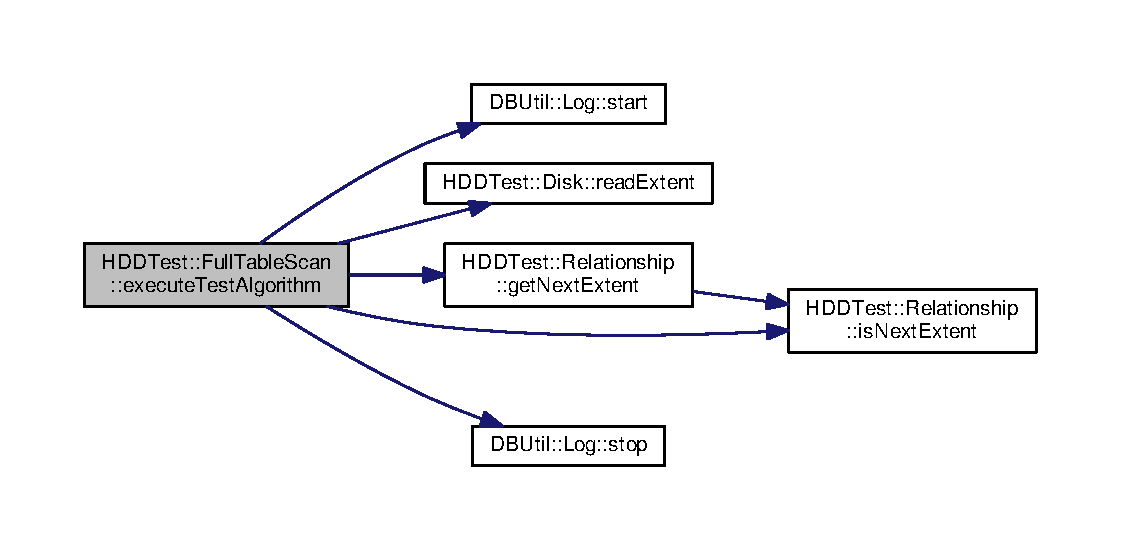
\includegraphics[width=350pt]{class_h_d_d_test_1_1_full_table_scan_a732473e7440538517ab2c1f6e9e636eb_cgraph}
\end{center}
\end{figure}




The documentation for this class was generated from the following files\-:\begin{DoxyCompactItemize}
\item 
src/\-Tests/\hyperlink{_full_table_scan_8cpp}{Full\-Table\-Scan.\-cpp}\item 
src/\-Tests/\hyperlink{_full_table_scan_8h}{Full\-Table\-Scan.\-h}\end{DoxyCompactItemize}

\hypertarget{class_h_d_d_test_1_1_index_scan}{\section{H\-D\-D\-Test\-:\-:Index\-Scan Class Reference}
\label{class_h_d_d_test_1_1_index_scan}\index{H\-D\-D\-Test\-::\-Index\-Scan@{H\-D\-D\-Test\-::\-Index\-Scan}}
}


{\ttfamily \#include $<$Index\-Scan.\-h$>$}



Inheritance diagram for H\-D\-D\-Test\-:\-:Index\-Scan\-:\nopagebreak
\begin{figure}[H]
\begin{center}
\leavevmode
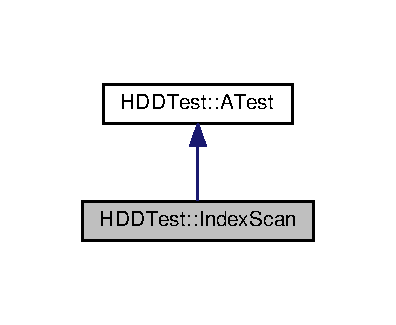
\includegraphics[width=190pt]{class_h_d_d_test_1_1_index_scan__inherit__graph}
\end{center}
\end{figure}


Collaboration diagram for H\-D\-D\-Test\-:\-:Index\-Scan\-:\nopagebreak
\begin{figure}[H]
\begin{center}
\leavevmode
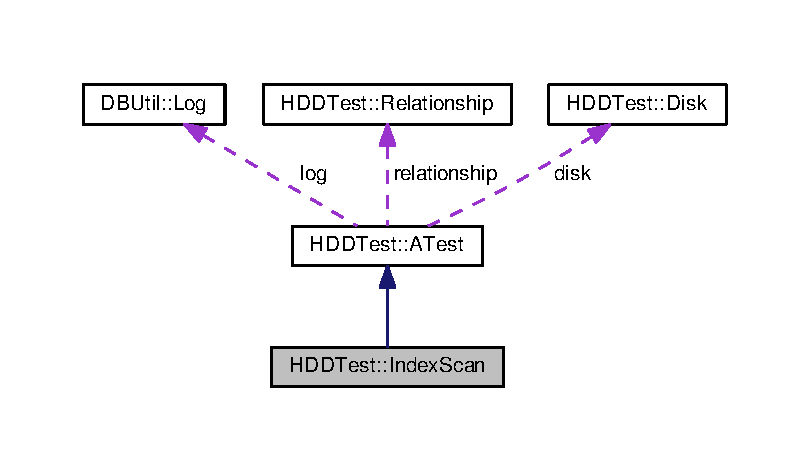
\includegraphics[width=350pt]{class_h_d_d_test_1_1_index_scan__coll__graph}
\end{center}
\end{figure}
\subsection*{Public Member Functions}
\begin{DoxyCompactItemize}
\item 
\hyperlink{class_h_d_d_test_1_1_index_scan_a30df1045c8296dd944bacac2bcee8692}{Index\-Scan} (std\-::string, \hyperlink{class_h_d_d_test_1_1_disk}{Disk} $\ast$, \hyperlink{class_h_d_d_test_1_1_relationship}{Relationship} $\ast$)
\item 
virtual \hyperlink{class_h_d_d_test_1_1_index_scan_afb5fc1d7594508c651e232cb249909e4}{$\sim$\-Index\-Scan} ()
\item 
void \hyperlink{class_h_d_d_test_1_1_index_scan_a63c295ffb3dd74515cf6c6583c9dc462}{execute\-Test\-Algorithm} () override
\end{DoxyCompactItemize}
\subsection*{Additional Inherited Members}


\subsection{Detailed Description}


Definition at line 15 of file Index\-Scan.\-h.



\subsection{Constructor \& Destructor Documentation}
\hypertarget{class_h_d_d_test_1_1_index_scan_a30df1045c8296dd944bacac2bcee8692}{\index{H\-D\-D\-Test\-::\-Index\-Scan@{H\-D\-D\-Test\-::\-Index\-Scan}!Index\-Scan@{Index\-Scan}}
\index{Index\-Scan@{Index\-Scan}!HDDTest::IndexScan@{H\-D\-D\-Test\-::\-Index\-Scan}}
\subsubsection[{Index\-Scan}]{\setlength{\rightskip}{0pt plus 5cm}H\-D\-D\-Test\-::\-Index\-Scan\-::\-Index\-Scan (
\begin{DoxyParamCaption}
\item[{std\-::string}]{name, }
\item[{{\bf Disk} $\ast$}]{disk, }
\item[{{\bf Relationship} $\ast$}]{relationship}
\end{DoxyParamCaption}
)}}\label{class_h_d_d_test_1_1_index_scan_a30df1045c8296dd944bacac2bcee8692}


Definition at line 14 of file Index\-Scan.\-cpp.

\hypertarget{class_h_d_d_test_1_1_index_scan_afb5fc1d7594508c651e232cb249909e4}{\index{H\-D\-D\-Test\-::\-Index\-Scan@{H\-D\-D\-Test\-::\-Index\-Scan}!$\sim$\-Index\-Scan@{$\sim$\-Index\-Scan}}
\index{$\sim$\-Index\-Scan@{$\sim$\-Index\-Scan}!HDDTest::IndexScan@{H\-D\-D\-Test\-::\-Index\-Scan}}
\subsubsection[{$\sim$\-Index\-Scan}]{\setlength{\rightskip}{0pt plus 5cm}H\-D\-D\-Test\-::\-Index\-Scan\-::$\sim$\-Index\-Scan (
\begin{DoxyParamCaption}
{}
\end{DoxyParamCaption}
)\hspace{0.3cm}{\ttfamily [virtual]}}}\label{class_h_d_d_test_1_1_index_scan_afb5fc1d7594508c651e232cb249909e4}


Definition at line 58 of file Index\-Scan.\-cpp.



\subsection{Member Function Documentation}
\hypertarget{class_h_d_d_test_1_1_index_scan_a63c295ffb3dd74515cf6c6583c9dc462}{\index{H\-D\-D\-Test\-::\-Index\-Scan@{H\-D\-D\-Test\-::\-Index\-Scan}!execute\-Test\-Algorithm@{execute\-Test\-Algorithm}}
\index{execute\-Test\-Algorithm@{execute\-Test\-Algorithm}!HDDTest::IndexScan@{H\-D\-D\-Test\-::\-Index\-Scan}}
\subsubsection[{execute\-Test\-Algorithm}]{\setlength{\rightskip}{0pt plus 5cm}void H\-D\-D\-Test\-::\-Index\-Scan\-::execute\-Test\-Algorithm (
\begin{DoxyParamCaption}
{}
\end{DoxyParamCaption}
)\hspace{0.3cm}{\ttfamily [override]}, {\ttfamily [virtual]}}}\label{class_h_d_d_test_1_1_index_scan_a63c295ffb3dd74515cf6c6583c9dc462}


Reimplemented from \hyperlink{class_h_d_d_test_1_1_a_test_a7dc054e211eccf42c03a6bb31d7fdc6e}{H\-D\-D\-Test\-::\-A\-Test}.



Definition at line 17 of file Index\-Scan.\-cpp.



Here is the call graph for this function\-:\nopagebreak
\begin{figure}[H]
\begin{center}
\leavevmode
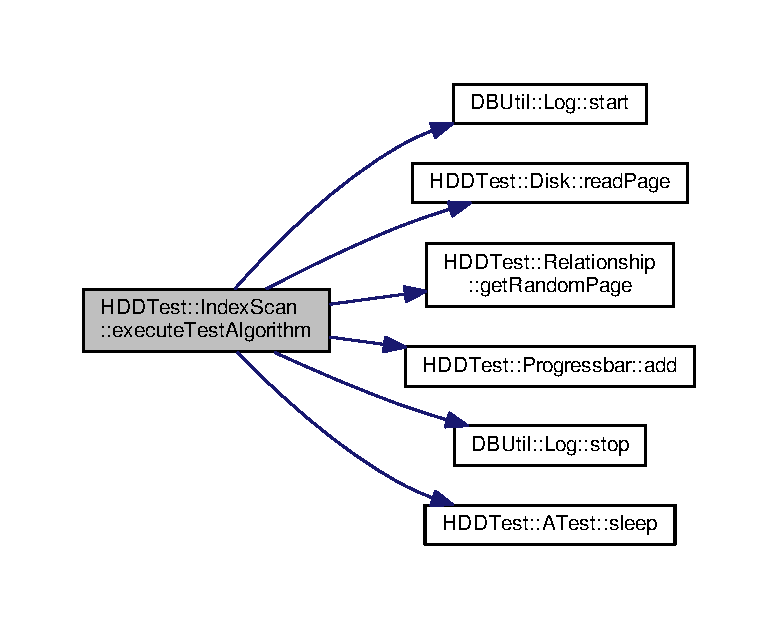
\includegraphics[width=350pt]{class_h_d_d_test_1_1_index_scan_a63c295ffb3dd74515cf6c6583c9dc462_cgraph}
\end{center}
\end{figure}




The documentation for this class was generated from the following files\-:\begin{DoxyCompactItemize}
\item 
src/\-Tests/\hyperlink{_index_scan_8h}{Index\-Scan.\-h}\item 
src/\-Tests/\hyperlink{_index_scan_8cpp}{Index\-Scan.\-cpp}\end{DoxyCompactItemize}

\hypertarget{class_h_d_d_test_1_1_index_write}{\section{H\-D\-D\-Test\-:\-:Index\-Write Class Reference}
\label{class_h_d_d_test_1_1_index_write}\index{H\-D\-D\-Test\-::\-Index\-Write@{H\-D\-D\-Test\-::\-Index\-Write}}
}


{\ttfamily \#include $<$Index\-Write.\-h$>$}



Inheritance diagram for H\-D\-D\-Test\-:\-:Index\-Write\-:
\nopagebreak
\begin{figure}[H]
\begin{center}
\leavevmode
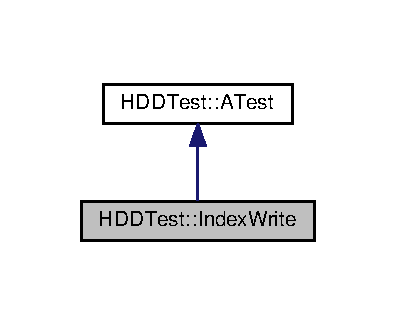
\includegraphics[width=190pt]{class_h_d_d_test_1_1_index_write__inherit__graph}
\end{center}
\end{figure}


Collaboration diagram for H\-D\-D\-Test\-:\-:Index\-Write\-:
\nopagebreak
\begin{figure}[H]
\begin{center}
\leavevmode
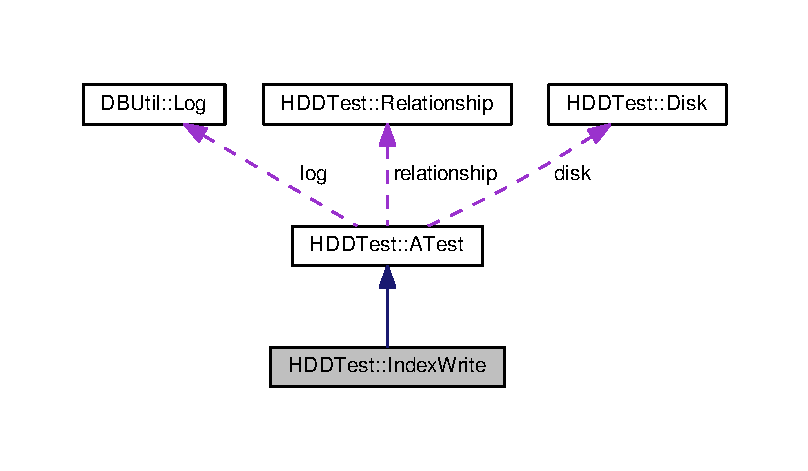
\includegraphics[width=350pt]{class_h_d_d_test_1_1_index_write__coll__graph}
\end{center}
\end{figure}
\subsection*{Public Member Functions}
\begin{DoxyCompactItemize}
\item 
\hyperlink{class_h_d_d_test_1_1_index_write_ad5adafd055f5090a353cc0d516720fda}{Index\-Write} (std\-::string, \hyperlink{class_h_d_d_test_1_1_disk}{Disk} $\ast$, \hyperlink{class_h_d_d_test_1_1_relationship}{Relationship} $\ast$)
\item 
virtual \hyperlink{class_h_d_d_test_1_1_index_write_ac936ba268793c1cf380668fa82382afa}{$\sim$\-Index\-Write} ()
\item 
void \hyperlink{class_h_d_d_test_1_1_index_write_afe685020b557ab773d4804d290cc361b}{execute\-Test\-Algorithm} () override
\end{DoxyCompactItemize}
\subsection*{Additional Inherited Members}


\subsection{Detailed Description}


Definition at line 15 of file Index\-Write.\-h.



\subsection{Constructor \& Destructor Documentation}
\hypertarget{class_h_d_d_test_1_1_index_write_ad5adafd055f5090a353cc0d516720fda}{\index{H\-D\-D\-Test\-::\-Index\-Write@{H\-D\-D\-Test\-::\-Index\-Write}!Index\-Write@{Index\-Write}}
\index{Index\-Write@{Index\-Write}!HDDTest::IndexWrite@{H\-D\-D\-Test\-::\-Index\-Write}}
\subsubsection[{Index\-Write}]{\setlength{\rightskip}{0pt plus 5cm}H\-D\-D\-Test\-::\-Index\-Write\-::\-Index\-Write (
\begin{DoxyParamCaption}
\item[{std\-::string}]{name, }
\item[{{\bf Disk} $\ast$}]{disk, }
\item[{{\bf Relationship} $\ast$}]{relationship}
\end{DoxyParamCaption}
)}}\label{class_h_d_d_test_1_1_index_write_ad5adafd055f5090a353cc0d516720fda}


Definition at line 14 of file Index\-Write.\-cpp.

\hypertarget{class_h_d_d_test_1_1_index_write_ac936ba268793c1cf380668fa82382afa}{\index{H\-D\-D\-Test\-::\-Index\-Write@{H\-D\-D\-Test\-::\-Index\-Write}!$\sim$\-Index\-Write@{$\sim$\-Index\-Write}}
\index{$\sim$\-Index\-Write@{$\sim$\-Index\-Write}!HDDTest::IndexWrite@{H\-D\-D\-Test\-::\-Index\-Write}}
\subsubsection[{$\sim$\-Index\-Write}]{\setlength{\rightskip}{0pt plus 5cm}H\-D\-D\-Test\-::\-Index\-Write\-::$\sim$\-Index\-Write (
\begin{DoxyParamCaption}
{}
\end{DoxyParamCaption}
)\hspace{0.3cm}{\ttfamily [virtual]}}}\label{class_h_d_d_test_1_1_index_write_ac936ba268793c1cf380668fa82382afa}


Definition at line 58 of file Index\-Write.\-cpp.



\subsection{Member Function Documentation}
\hypertarget{class_h_d_d_test_1_1_index_write_afe685020b557ab773d4804d290cc361b}{\index{H\-D\-D\-Test\-::\-Index\-Write@{H\-D\-D\-Test\-::\-Index\-Write}!execute\-Test\-Algorithm@{execute\-Test\-Algorithm}}
\index{execute\-Test\-Algorithm@{execute\-Test\-Algorithm}!HDDTest::IndexWrite@{H\-D\-D\-Test\-::\-Index\-Write}}
\subsubsection[{execute\-Test\-Algorithm}]{\setlength{\rightskip}{0pt plus 5cm}void H\-D\-D\-Test\-::\-Index\-Write\-::execute\-Test\-Algorithm (
\begin{DoxyParamCaption}
{}
\end{DoxyParamCaption}
)\hspace{0.3cm}{\ttfamily [override]}, {\ttfamily [virtual]}}}\label{class_h_d_d_test_1_1_index_write_afe685020b557ab773d4804d290cc361b}


Reimplemented from \hyperlink{class_h_d_d_test_1_1_a_test_a7dc054e211eccf42c03a6bb31d7fdc6e}{H\-D\-D\-Test\-::\-A\-Test}.



Definition at line 17 of file Index\-Write.\-cpp.



Here is the call graph for this function\-:
\nopagebreak
\begin{figure}[H]
\begin{center}
\leavevmode
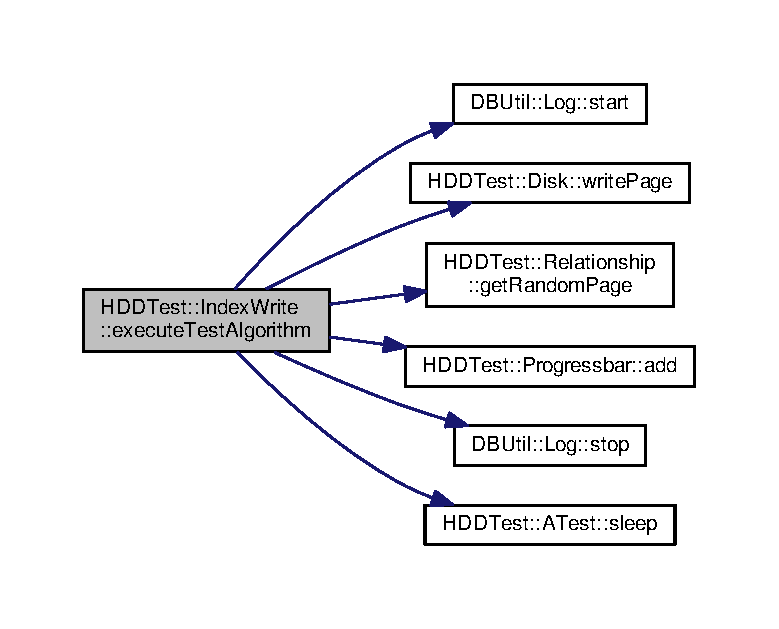
\includegraphics[width=350pt]{class_h_d_d_test_1_1_index_write_afe685020b557ab773d4804d290cc361b_cgraph}
\end{center}
\end{figure}




The documentation for this class was generated from the following files\-:\begin{DoxyCompactItemize}
\item 
src/\-Tests/\hyperlink{_index_write_8h}{Index\-Write.\-h}\item 
src/\-Tests/\hyperlink{_index_write_8cpp}{Index\-Write.\-cpp}\end{DoxyCompactItemize}

\hypertarget{class_h_d_d_test_1_1_layout}{\section{H\-D\-D\-Test\-:\-:Layout Class Reference}
\label{class_h_d_d_test_1_1_layout}\index{H\-D\-D\-Test\-::\-Layout@{H\-D\-D\-Test\-::\-Layout}}
}


{\ttfamily \#include $<$Layout.\-h$>$}

\subsection*{Public Member Functions}
\begin{DoxyCompactItemize}
\item 
\hyperlink{class_h_d_d_test_1_1_layout_a65643db5707927aefc6069735da99a21}{Layout} (struct \hyperlink{struct_h_d_d_test_1_1_layout_settings}{Layout\-Settings})
\item 
virtual \hyperlink{class_h_d_d_test_1_1_layout_aa12e04fdf79d0976d2020c4ee6c9305e}{$\sim$\-Layout} ()
\item 
void \hyperlink{class_h_d_d_test_1_1_layout_afeb15d353e1bb5b8089ce0fd35d00c44}{create\-Relationships} (std\-::vector$<$ struct \hyperlink{struct_h_d_d_test_1_1_relationship_config}{Relationship\-Config} $>$)
\item 
\hyperlink{class_h_d_d_test_1_1_relationship}{H\-D\-D\-Test\-::\-Relationship} $\ast$ \hyperlink{class_h_d_d_test_1_1_layout_af7aef9c0227433e1cfc6252cb85e8dc3}{get\-Relationship} (std\-::string)
\end{DoxyCompactItemize}
\subsection*{Public Attributes}
\begin{DoxyCompactItemize}
\item 
uint64\-\_\-t \hyperlink{class_h_d_d_test_1_1_layout_aeba9e8e44b4ba70259ff783680b988fe}{disk\-Start}
\end{DoxyCompactItemize}


\subsection{Detailed Description}


Definition at line 33 of file Layout.\-h.



\subsection{Constructor \& Destructor Documentation}
\hypertarget{class_h_d_d_test_1_1_layout_a65643db5707927aefc6069735da99a21}{\index{H\-D\-D\-Test\-::\-Layout@{H\-D\-D\-Test\-::\-Layout}!Layout@{Layout}}
\index{Layout@{Layout}!HDDTest::Layout@{H\-D\-D\-Test\-::\-Layout}}
\subsubsection[{Layout}]{\setlength{\rightskip}{0pt plus 5cm}H\-D\-D\-Test\-::\-Layout\-::\-Layout (
\begin{DoxyParamCaption}
\item[{struct {\bf Layout\-Settings}}]{layout\-Setting}
\end{DoxyParamCaption}
)}}\label{class_h_d_d_test_1_1_layout_a65643db5707927aefc6069735da99a21}


Definition at line 13 of file Layout.\-cpp.



Here is the call graph for this function\-:\nopagebreak
\begin{figure}[H]
\begin{center}
\leavevmode
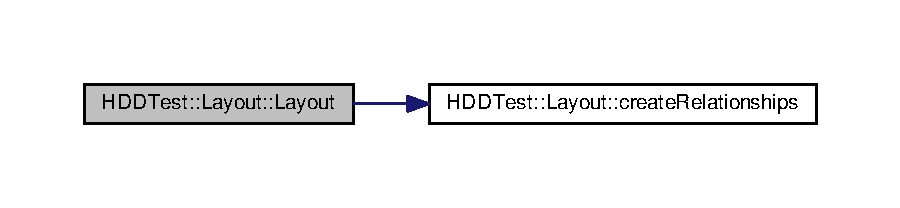
\includegraphics[width=350pt]{class_h_d_d_test_1_1_layout_a65643db5707927aefc6069735da99a21_cgraph}
\end{center}
\end{figure}


\hypertarget{class_h_d_d_test_1_1_layout_aa12e04fdf79d0976d2020c4ee6c9305e}{\index{H\-D\-D\-Test\-::\-Layout@{H\-D\-D\-Test\-::\-Layout}!$\sim$\-Layout@{$\sim$\-Layout}}
\index{$\sim$\-Layout@{$\sim$\-Layout}!HDDTest::Layout@{H\-D\-D\-Test\-::\-Layout}}
\subsubsection[{$\sim$\-Layout}]{\setlength{\rightskip}{0pt plus 5cm}H\-D\-D\-Test\-::\-Layout\-::$\sim$\-Layout (
\begin{DoxyParamCaption}
{}
\end{DoxyParamCaption}
)\hspace{0.3cm}{\ttfamily [virtual]}}}\label{class_h_d_d_test_1_1_layout_aa12e04fdf79d0976d2020c4ee6c9305e}


Definition at line 21 of file Layout.\-cpp.



\subsection{Member Function Documentation}
\hypertarget{class_h_d_d_test_1_1_layout_afeb15d353e1bb5b8089ce0fd35d00c44}{\index{H\-D\-D\-Test\-::\-Layout@{H\-D\-D\-Test\-::\-Layout}!create\-Relationships@{create\-Relationships}}
\index{create\-Relationships@{create\-Relationships}!HDDTest::Layout@{H\-D\-D\-Test\-::\-Layout}}
\subsubsection[{create\-Relationships}]{\setlength{\rightskip}{0pt plus 5cm}void H\-D\-D\-Test\-::\-Layout\-::create\-Relationships (
\begin{DoxyParamCaption}
\item[{std\-::vector$<$ struct {\bf Relationship\-Config} $>$}]{}
\end{DoxyParamCaption}
)}}\label{class_h_d_d_test_1_1_layout_afeb15d353e1bb5b8089ce0fd35d00c44}


Definition at line 27 of file Layout.\-cpp.



Here is the caller graph for this function\-:\nopagebreak
\begin{figure}[H]
\begin{center}
\leavevmode
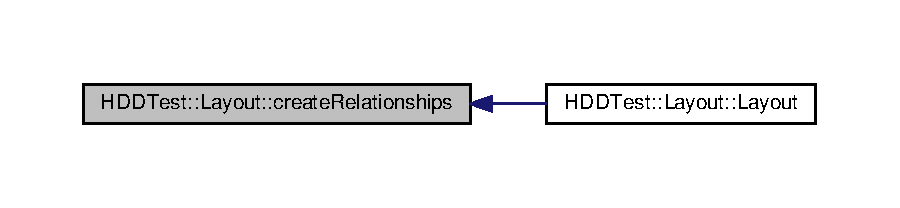
\includegraphics[width=350pt]{class_h_d_d_test_1_1_layout_afeb15d353e1bb5b8089ce0fd35d00c44_icgraph}
\end{center}
\end{figure}


\hypertarget{class_h_d_d_test_1_1_layout_af7aef9c0227433e1cfc6252cb85e8dc3}{\index{H\-D\-D\-Test\-::\-Layout@{H\-D\-D\-Test\-::\-Layout}!get\-Relationship@{get\-Relationship}}
\index{get\-Relationship@{get\-Relationship}!HDDTest::Layout@{H\-D\-D\-Test\-::\-Layout}}
\subsubsection[{get\-Relationship}]{\setlength{\rightskip}{0pt plus 5cm}{\bf H\-D\-D\-Test\-::\-Relationship} $\ast$ H\-D\-D\-Test\-::\-Layout\-::get\-Relationship (
\begin{DoxyParamCaption}
\item[{std\-::string}]{name}
\end{DoxyParamCaption}
)}}\label{class_h_d_d_test_1_1_layout_af7aef9c0227433e1cfc6252cb85e8dc3}


Definition at line 62 of file Layout.\-cpp.



Here is the caller graph for this function\-:\nopagebreak
\begin{figure}[H]
\begin{center}
\leavevmode
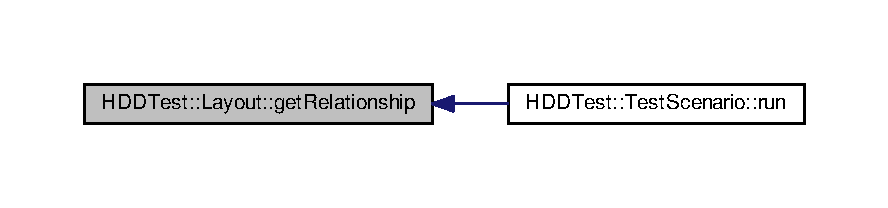
\includegraphics[width=350pt]{class_h_d_d_test_1_1_layout_af7aef9c0227433e1cfc6252cb85e8dc3_icgraph}
\end{center}
\end{figure}




\subsection{Member Data Documentation}
\hypertarget{class_h_d_d_test_1_1_layout_aeba9e8e44b4ba70259ff783680b988fe}{\index{H\-D\-D\-Test\-::\-Layout@{H\-D\-D\-Test\-::\-Layout}!disk\-Start@{disk\-Start}}
\index{disk\-Start@{disk\-Start}!HDDTest::Layout@{H\-D\-D\-Test\-::\-Layout}}
\subsubsection[{disk\-Start}]{\setlength{\rightskip}{0pt plus 5cm}uint64\-\_\-t H\-D\-D\-Test\-::\-Layout\-::disk\-Start}}\label{class_h_d_d_test_1_1_layout_aeba9e8e44b4ba70259ff783680b988fe}


Definition at line 41 of file Layout.\-h.



The documentation for this class was generated from the following files\-:\begin{DoxyCompactItemize}
\item 
src/\-Layout/\hyperlink{_layout_8h}{Layout.\-h}\item 
src/\-Layout/\hyperlink{_layout_8cpp}{Layout.\-cpp}\end{DoxyCompactItemize}

\hypertarget{struct_h_d_d_test_1_1_layout_settings}{\section{H\-D\-D\-Test\-:\-:Layout\-Settings Struct Reference}
\label{struct_h_d_d_test_1_1_layout_settings}\index{H\-D\-D\-Test\-::\-Layout\-Settings@{H\-D\-D\-Test\-::\-Layout\-Settings}}
}


{\ttfamily \#include $<$Layout.\-h$>$}

\subsection*{Public Attributes}
\begin{DoxyCompactItemize}
\item 
std\-::string \hyperlink{struct_h_d_d_test_1_1_layout_settings_ae44172312461b7fa707c3c76dcbf834a}{mode}
\item 
uint64\-\_\-t \hyperlink{struct_h_d_d_test_1_1_layout_settings_ac0a3416abc480fde8b194b02cbfcad25}{page\-Size\-In\-K\-B}
\item 
uint64\-\_\-t \hyperlink{struct_h_d_d_test_1_1_layout_settings_aea0e0ec07c3ddc2dd198345689f6899e}{pages\-Per\-Extent}
\item 
std\-::vector$<$ struct \\*
\hyperlink{struct_h_d_d_test_1_1_relationship_config}{Relationship\-Config} $>$ \hyperlink{struct_h_d_d_test_1_1_layout_settings_a9d2aea674708a168136bd3aba5a27be9}{relationships}
\end{DoxyCompactItemize}


\subsection{Detailed Description}


Definition at line 25 of file Layout.\-h.



\subsection{Member Data Documentation}
\hypertarget{struct_h_d_d_test_1_1_layout_settings_ae44172312461b7fa707c3c76dcbf834a}{\index{H\-D\-D\-Test\-::\-Layout\-Settings@{H\-D\-D\-Test\-::\-Layout\-Settings}!mode@{mode}}
\index{mode@{mode}!HDDTest::LayoutSettings@{H\-D\-D\-Test\-::\-Layout\-Settings}}
\subsubsection[{mode}]{\setlength{\rightskip}{0pt plus 5cm}std\-::string H\-D\-D\-Test\-::\-Layout\-Settings\-::mode}}\label{struct_h_d_d_test_1_1_layout_settings_ae44172312461b7fa707c3c76dcbf834a}


Definition at line 27 of file Layout.\-h.

\hypertarget{struct_h_d_d_test_1_1_layout_settings_ac0a3416abc480fde8b194b02cbfcad25}{\index{H\-D\-D\-Test\-::\-Layout\-Settings@{H\-D\-D\-Test\-::\-Layout\-Settings}!page\-Size\-In\-K\-B@{page\-Size\-In\-K\-B}}
\index{page\-Size\-In\-K\-B@{page\-Size\-In\-K\-B}!HDDTest::LayoutSettings@{H\-D\-D\-Test\-::\-Layout\-Settings}}
\subsubsection[{page\-Size\-In\-K\-B}]{\setlength{\rightskip}{0pt plus 5cm}uint64\-\_\-t H\-D\-D\-Test\-::\-Layout\-Settings\-::page\-Size\-In\-K\-B}}\label{struct_h_d_d_test_1_1_layout_settings_ac0a3416abc480fde8b194b02cbfcad25}


Definition at line 28 of file Layout.\-h.

\hypertarget{struct_h_d_d_test_1_1_layout_settings_aea0e0ec07c3ddc2dd198345689f6899e}{\index{H\-D\-D\-Test\-::\-Layout\-Settings@{H\-D\-D\-Test\-::\-Layout\-Settings}!pages\-Per\-Extent@{pages\-Per\-Extent}}
\index{pages\-Per\-Extent@{pages\-Per\-Extent}!HDDTest::LayoutSettings@{H\-D\-D\-Test\-::\-Layout\-Settings}}
\subsubsection[{pages\-Per\-Extent}]{\setlength{\rightskip}{0pt plus 5cm}uint64\-\_\-t H\-D\-D\-Test\-::\-Layout\-Settings\-::pages\-Per\-Extent}}\label{struct_h_d_d_test_1_1_layout_settings_aea0e0ec07c3ddc2dd198345689f6899e}


Definition at line 29 of file Layout.\-h.

\hypertarget{struct_h_d_d_test_1_1_layout_settings_a9d2aea674708a168136bd3aba5a27be9}{\index{H\-D\-D\-Test\-::\-Layout\-Settings@{H\-D\-D\-Test\-::\-Layout\-Settings}!relationships@{relationships}}
\index{relationships@{relationships}!HDDTest::LayoutSettings@{H\-D\-D\-Test\-::\-Layout\-Settings}}
\subsubsection[{relationships}]{\setlength{\rightskip}{0pt plus 5cm}std\-::vector$<$struct {\bf Relationship\-Config}$>$ H\-D\-D\-Test\-::\-Layout\-Settings\-::relationships}}\label{struct_h_d_d_test_1_1_layout_settings_a9d2aea674708a168136bd3aba5a27be9}


Definition at line 30 of file Layout.\-h.



The documentation for this struct was generated from the following file\-:\begin{DoxyCompactItemize}
\item 
src/\-Layout/\hyperlink{_layout_8h}{Layout.\-h}\end{DoxyCompactItemize}

\hypertarget{class_d_b_util_1_1_log}{\section{D\-B\-Util\-:\-:Log Class Reference}
\label{class_d_b_util_1_1_log}\index{D\-B\-Util\-::\-Log@{D\-B\-Util\-::\-Log}}
}


{\ttfamily \#include $<$Log.\-h$>$}

\subsection*{Public Member Functions}
\begin{DoxyCompactItemize}
\item 
\hyperlink{class_d_b_util_1_1_log_afc06f47293c880700ed2c92abdbaef9e}{Log} ()
\item 
virtual \hyperlink{class_d_b_util_1_1_log_a2d17e870ff4661b670ce9bb10d4c7e82}{$\sim$\-Log} ()
\item 
void \hyperlink{class_d_b_util_1_1_log_a64073692efb1f1b5bde7af7faee62e8c}{start} ()
\item 
void \hyperlink{class_d_b_util_1_1_log_ae6a543277090bfe89db07e49a71ec4e1}{stop} (uint64\-\_\-t)
\item 
void \hyperlink{class_d_b_util_1_1_log_a56f0e1120dcb0000063664f5efe39453}{write} (std\-::string)
\end{DoxyCompactItemize}


\subsection{Detailed Description}


Definition at line 25 of file Log.\-h.



\subsection{Constructor \& Destructor Documentation}
\hypertarget{class_d_b_util_1_1_log_afc06f47293c880700ed2c92abdbaef9e}{\index{D\-B\-Util\-::\-Log@{D\-B\-Util\-::\-Log}!Log@{Log}}
\index{Log@{Log}!DBUtil::Log@{D\-B\-Util\-::\-Log}}
\subsubsection[{Log}]{\setlength{\rightskip}{0pt plus 5cm}D\-B\-Util\-::\-Log\-::\-Log (
\begin{DoxyParamCaption}
{}
\end{DoxyParamCaption}
)}}\label{class_d_b_util_1_1_log_afc06f47293c880700ed2c92abdbaef9e}


Definition at line 17 of file Log.\-cpp.

\hypertarget{class_d_b_util_1_1_log_a2d17e870ff4661b670ce9bb10d4c7e82}{\index{D\-B\-Util\-::\-Log@{D\-B\-Util\-::\-Log}!$\sim$\-Log@{$\sim$\-Log}}
\index{$\sim$\-Log@{$\sim$\-Log}!DBUtil::Log@{D\-B\-Util\-::\-Log}}
\subsubsection[{$\sim$\-Log}]{\setlength{\rightskip}{0pt plus 5cm}D\-B\-Util\-::\-Log\-::$\sim$\-Log (
\begin{DoxyParamCaption}
{}
\end{DoxyParamCaption}
)\hspace{0.3cm}{\ttfamily [virtual]}}}\label{class_d_b_util_1_1_log_a2d17e870ff4661b670ce9bb10d4c7e82}


Definition at line 23 of file Log.\-cpp.



\subsection{Member Function Documentation}
\hypertarget{class_d_b_util_1_1_log_a64073692efb1f1b5bde7af7faee62e8c}{\index{D\-B\-Util\-::\-Log@{D\-B\-Util\-::\-Log}!start@{start}}
\index{start@{start}!DBUtil::Log@{D\-B\-Util\-::\-Log}}
\subsubsection[{start}]{\setlength{\rightskip}{0pt plus 5cm}void D\-B\-Util\-::\-Log\-::start (
\begin{DoxyParamCaption}
{}
\end{DoxyParamCaption}
)}}\label{class_d_b_util_1_1_log_a64073692efb1f1b5bde7af7faee62e8c}


Definition at line 28 of file Log.\-cpp.



Here is the caller graph for this function\-:\nopagebreak
\begin{figure}[H]
\begin{center}
\leavevmode
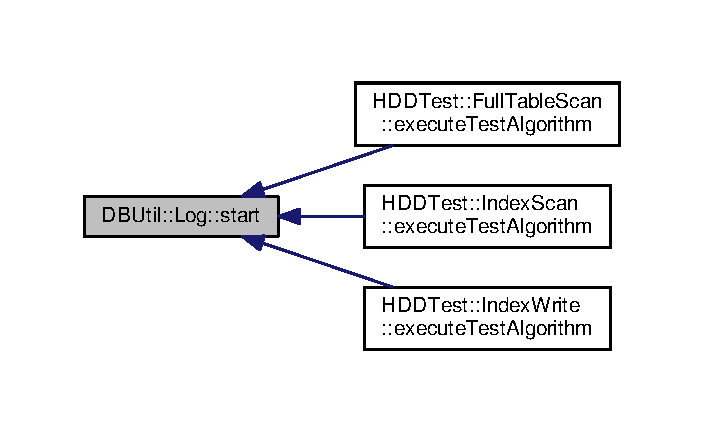
\includegraphics[width=338pt]{class_d_b_util_1_1_log_a64073692efb1f1b5bde7af7faee62e8c_icgraph}
\end{center}
\end{figure}


\hypertarget{class_d_b_util_1_1_log_ae6a543277090bfe89db07e49a71ec4e1}{\index{D\-B\-Util\-::\-Log@{D\-B\-Util\-::\-Log}!stop@{stop}}
\index{stop@{stop}!DBUtil::Log@{D\-B\-Util\-::\-Log}}
\subsubsection[{stop}]{\setlength{\rightskip}{0pt plus 5cm}void D\-B\-Util\-::\-Log\-::stop (
\begin{DoxyParamCaption}
\item[{uint64\-\_\-t}]{size}
\end{DoxyParamCaption}
)}}\label{class_d_b_util_1_1_log_ae6a543277090bfe89db07e49a71ec4e1}


Definition at line 33 of file Log.\-cpp.



Here is the caller graph for this function\-:\nopagebreak
\begin{figure}[H]
\begin{center}
\leavevmode
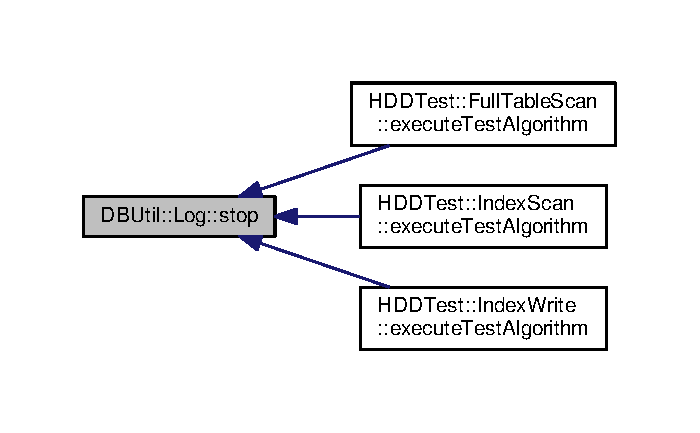
\includegraphics[width=336pt]{class_d_b_util_1_1_log_ae6a543277090bfe89db07e49a71ec4e1_icgraph}
\end{center}
\end{figure}


\hypertarget{class_d_b_util_1_1_log_a56f0e1120dcb0000063664f5efe39453}{\index{D\-B\-Util\-::\-Log@{D\-B\-Util\-::\-Log}!write@{write}}
\index{write@{write}!DBUtil::Log@{D\-B\-Util\-::\-Log}}
\subsubsection[{write}]{\setlength{\rightskip}{0pt plus 5cm}void D\-B\-Util\-::\-Log\-::write (
\begin{DoxyParamCaption}
\item[{std\-::string}]{name}
\end{DoxyParamCaption}
)}}\label{class_d_b_util_1_1_log_a56f0e1120dcb0000063664f5efe39453}


Definition at line 43 of file Log.\-cpp.



Here is the caller graph for this function\-:\nopagebreak
\begin{figure}[H]
\begin{center}
\leavevmode
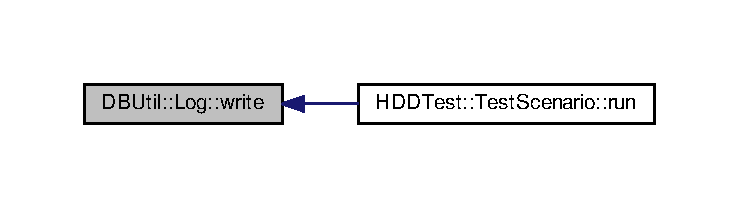
\includegraphics[width=350pt]{class_d_b_util_1_1_log_a56f0e1120dcb0000063664f5efe39453_icgraph}
\end{center}
\end{figure}




The documentation for this class was generated from the following files\-:\begin{DoxyCompactItemize}
\item 
src/\-Util/\hyperlink{_log_8h}{Log.\-h}\item 
src/\-Util/\hyperlink{_log_8cpp}{Log.\-cpp}\end{DoxyCompactItemize}

\hypertarget{struct_d_b_util_1_1measurement}{\section{D\-B\-Util\-:\-:measurement Struct Reference}
\label{struct_d_b_util_1_1measurement}\index{D\-B\-Util\-::measurement@{D\-B\-Util\-::measurement}}
}


{\ttfamily \#include $<$Log.\-h$>$}

\subsection*{Public Attributes}
\begin{DoxyCompactItemize}
\item 
uint64\-\_\-t \hyperlink{struct_d_b_util_1_1measurement_a91c62eb1fa3de2e3be1a9127c5822b96}{duration}
\item 
uint64\-\_\-t \hyperlink{struct_d_b_util_1_1measurement_aa1de62e639b640d4dadb2fd6d0f95d9e}{size}
\end{DoxyCompactItemize}


\subsection{Detailed Description}


Definition at line 19 of file Log.\-h.



\subsection{Member Data Documentation}
\hypertarget{struct_d_b_util_1_1measurement_a91c62eb1fa3de2e3be1a9127c5822b96}{\index{D\-B\-Util\-::measurement@{D\-B\-Util\-::measurement}!duration@{duration}}
\index{duration@{duration}!DBUtil::measurement@{D\-B\-Util\-::measurement}}
\subsubsection[{duration}]{\setlength{\rightskip}{0pt plus 5cm}uint64\-\_\-t D\-B\-Util\-::measurement\-::duration}}\label{struct_d_b_util_1_1measurement_a91c62eb1fa3de2e3be1a9127c5822b96}


Definition at line 21 of file Log.\-h.

\hypertarget{struct_d_b_util_1_1measurement_aa1de62e639b640d4dadb2fd6d0f95d9e}{\index{D\-B\-Util\-::measurement@{D\-B\-Util\-::measurement}!size@{size}}
\index{size@{size}!DBUtil::measurement@{D\-B\-Util\-::measurement}}
\subsubsection[{size}]{\setlength{\rightskip}{0pt plus 5cm}uint64\-\_\-t D\-B\-Util\-::measurement\-::size}}\label{struct_d_b_util_1_1measurement_aa1de62e639b640d4dadb2fd6d0f95d9e}


Definition at line 22 of file Log.\-h.



The documentation for this struct was generated from the following file\-:\begin{DoxyCompactItemize}
\item 
src/\-Util/\hyperlink{_log_8h}{Log.\-h}\end{DoxyCompactItemize}

\hypertarget{class_h_d_d_test_1_1_progressbar}{\section{H\-D\-D\-Test\-:\-:Progressbar Class Reference}
\label{class_h_d_d_test_1_1_progressbar}\index{H\-D\-D\-Test\-::\-Progressbar@{H\-D\-D\-Test\-::\-Progressbar}}
}


{\ttfamily \#include $<$Progressbar.\-h$>$}

\subsection*{Public Member Functions}
\begin{DoxyCompactItemize}
\item 
\hyperlink{class_h_d_d_test_1_1_progressbar_ae8156d41aec4243b1328b62361965af1}{Progressbar} (std\-::string, uint64\-\_\-t)
\item 
void \hyperlink{class_h_d_d_test_1_1_progressbar_a031bb6b1e7a3305d441bc10353c37966}{add} (uint64\-\_\-t)
\item 
virtual \hyperlink{class_h_d_d_test_1_1_progressbar_a0abee569b47da1c25a8aef42339dc5f2}{$\sim$\-Progressbar} ()
\end{DoxyCompactItemize}
\subsection*{Public Attributes}
\begin{DoxyCompactItemize}
\item 
uint64\-\_\-t \hyperlink{class_h_d_d_test_1_1_progressbar_a611fb784d62df0f9f2d56ad90e15c47c}{total}
\item 
uint64\-\_\-t \hyperlink{class_h_d_d_test_1_1_progressbar_a8064f75e6a8ad05753bbff8752d6a5a7}{current}
\item 
int \hyperlink{class_h_d_d_test_1_1_progressbar_a754f1137a1b68fced60aebfc87269a84}{bar\-Width}
\item 
std\-::string \hyperlink{class_h_d_d_test_1_1_progressbar_a07e67985ad3a30bee17d36014a56b328}{name}
\end{DoxyCompactItemize}


\subsection{Detailed Description}


Definition at line 15 of file Progressbar.\-h.



\subsection{Constructor \& Destructor Documentation}
\hypertarget{class_h_d_d_test_1_1_progressbar_ae8156d41aec4243b1328b62361965af1}{\index{H\-D\-D\-Test\-::\-Progressbar@{H\-D\-D\-Test\-::\-Progressbar}!Progressbar@{Progressbar}}
\index{Progressbar@{Progressbar}!HDDTest::Progressbar@{H\-D\-D\-Test\-::\-Progressbar}}
\subsubsection[{Progressbar}]{\setlength{\rightskip}{0pt plus 5cm}H\-D\-D\-Test\-::\-Progressbar\-::\-Progressbar (
\begin{DoxyParamCaption}
\item[{std\-::string}]{name, }
\item[{uint64\-\_\-t}]{total}
\end{DoxyParamCaption}
)}}\label{class_h_d_d_test_1_1_progressbar_ae8156d41aec4243b1328b62361965af1}


Definition at line 14 of file Progressbar.\-cpp.

\hypertarget{class_h_d_d_test_1_1_progressbar_a0abee569b47da1c25a8aef42339dc5f2}{\index{H\-D\-D\-Test\-::\-Progressbar@{H\-D\-D\-Test\-::\-Progressbar}!$\sim$\-Progressbar@{$\sim$\-Progressbar}}
\index{$\sim$\-Progressbar@{$\sim$\-Progressbar}!HDDTest::Progressbar@{H\-D\-D\-Test\-::\-Progressbar}}
\subsubsection[{$\sim$\-Progressbar}]{\setlength{\rightskip}{0pt plus 5cm}H\-D\-D\-Test\-::\-Progressbar\-::$\sim$\-Progressbar (
\begin{DoxyParamCaption}
{}
\end{DoxyParamCaption}
)\hspace{0.3cm}{\ttfamily [virtual]}}}\label{class_h_d_d_test_1_1_progressbar_a0abee569b47da1c25a8aef42339dc5f2}


Definition at line 48 of file Progressbar.\-cpp.



\subsection{Member Function Documentation}
\hypertarget{class_h_d_d_test_1_1_progressbar_a031bb6b1e7a3305d441bc10353c37966}{\index{H\-D\-D\-Test\-::\-Progressbar@{H\-D\-D\-Test\-::\-Progressbar}!add@{add}}
\index{add@{add}!HDDTest::Progressbar@{H\-D\-D\-Test\-::\-Progressbar}}
\subsubsection[{add}]{\setlength{\rightskip}{0pt plus 5cm}void H\-D\-D\-Test\-::\-Progressbar\-::add (
\begin{DoxyParamCaption}
\item[{uint64\-\_\-t}]{addition}
\end{DoxyParamCaption}
)}}\label{class_h_d_d_test_1_1_progressbar_a031bb6b1e7a3305d441bc10353c37966}


Definition at line 24 of file Progressbar.\-cpp.



Here is the caller graph for this function\-:
\nopagebreak
\begin{figure}[H]
\begin{center}
\leavevmode
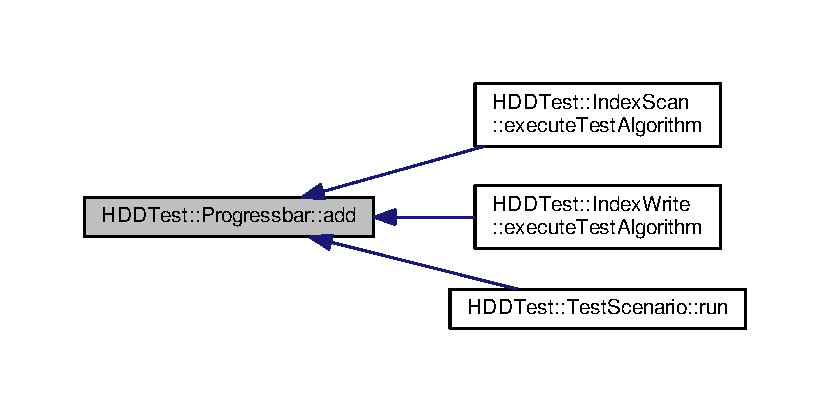
\includegraphics[width=350pt]{class_h_d_d_test_1_1_progressbar_a031bb6b1e7a3305d441bc10353c37966_icgraph}
\end{center}
\end{figure}




\subsection{Member Data Documentation}
\hypertarget{class_h_d_d_test_1_1_progressbar_a754f1137a1b68fced60aebfc87269a84}{\index{H\-D\-D\-Test\-::\-Progressbar@{H\-D\-D\-Test\-::\-Progressbar}!bar\-Width@{bar\-Width}}
\index{bar\-Width@{bar\-Width}!HDDTest::Progressbar@{H\-D\-D\-Test\-::\-Progressbar}}
\subsubsection[{bar\-Width}]{\setlength{\rightskip}{0pt plus 5cm}int H\-D\-D\-Test\-::\-Progressbar\-::bar\-Width}}\label{class_h_d_d_test_1_1_progressbar_a754f1137a1b68fced60aebfc87269a84}


Definition at line 22 of file Progressbar.\-h.

\hypertarget{class_h_d_d_test_1_1_progressbar_a8064f75e6a8ad05753bbff8752d6a5a7}{\index{H\-D\-D\-Test\-::\-Progressbar@{H\-D\-D\-Test\-::\-Progressbar}!current@{current}}
\index{current@{current}!HDDTest::Progressbar@{H\-D\-D\-Test\-::\-Progressbar}}
\subsubsection[{current}]{\setlength{\rightskip}{0pt plus 5cm}uint64\-\_\-t H\-D\-D\-Test\-::\-Progressbar\-::current}}\label{class_h_d_d_test_1_1_progressbar_a8064f75e6a8ad05753bbff8752d6a5a7}


Definition at line 21 of file Progressbar.\-h.

\hypertarget{class_h_d_d_test_1_1_progressbar_a07e67985ad3a30bee17d36014a56b328}{\index{H\-D\-D\-Test\-::\-Progressbar@{H\-D\-D\-Test\-::\-Progressbar}!name@{name}}
\index{name@{name}!HDDTest::Progressbar@{H\-D\-D\-Test\-::\-Progressbar}}
\subsubsection[{name}]{\setlength{\rightskip}{0pt plus 5cm}std\-::string H\-D\-D\-Test\-::\-Progressbar\-::name}}\label{class_h_d_d_test_1_1_progressbar_a07e67985ad3a30bee17d36014a56b328}


Definition at line 23 of file Progressbar.\-h.

\hypertarget{class_h_d_d_test_1_1_progressbar_a611fb784d62df0f9f2d56ad90e15c47c}{\index{H\-D\-D\-Test\-::\-Progressbar@{H\-D\-D\-Test\-::\-Progressbar}!total@{total}}
\index{total@{total}!HDDTest::Progressbar@{H\-D\-D\-Test\-::\-Progressbar}}
\subsubsection[{total}]{\setlength{\rightskip}{0pt plus 5cm}uint64\-\_\-t H\-D\-D\-Test\-::\-Progressbar\-::total}}\label{class_h_d_d_test_1_1_progressbar_a611fb784d62df0f9f2d56ad90e15c47c}


Definition at line 20 of file Progressbar.\-h.



The documentation for this class was generated from the following files\-:\begin{DoxyCompactItemize}
\item 
src/\-Util/\hyperlink{_progressbar_8h}{Progressbar.\-h}\item 
src/\-Util/\hyperlink{_progressbar_8cpp}{Progressbar.\-cpp}\end{DoxyCompactItemize}

\hypertarget{class_h_d_d_test_1_1_randomizer}{\section{H\-D\-D\-Test\-:\-:Randomizer Class Reference}
\label{class_h_d_d_test_1_1_randomizer}\index{H\-D\-D\-Test\-::\-Randomizer@{H\-D\-D\-Test\-::\-Randomizer}}
}


{\ttfamily \#include $<$Randomizer.\-h$>$}

\subsection*{Static Public Member Functions}
\begin{DoxyCompactItemize}
\item 
static void \hyperlink{class_h_d_d_test_1_1_randomizer_af2b09f326a10a75f53a8c3655e79c4cc}{seed} (uint64\-\_\-t new\-\_\-seed=std\-::mt19937\-\_\-64\-::default\-\_\-seed)
\item 
static uint64\-\_\-t \hyperlink{class_h_d_d_test_1_1_randomizer_ae6a1aa07280dc34dc99cc2b74b650624}{get} ()
\end{DoxyCompactItemize}


\subsection{Detailed Description}


Definition at line 16 of file Randomizer.\-h.



\subsection{Member Function Documentation}
\hypertarget{class_h_d_d_test_1_1_randomizer_ae6a1aa07280dc34dc99cc2b74b650624}{\index{H\-D\-D\-Test\-::\-Randomizer@{H\-D\-D\-Test\-::\-Randomizer}!get@{get}}
\index{get@{get}!HDDTest::Randomizer@{H\-D\-D\-Test\-::\-Randomizer}}
\subsubsection[{get}]{\setlength{\rightskip}{0pt plus 5cm}static uint64\-\_\-t H\-D\-D\-Test\-::\-Randomizer\-::get (
\begin{DoxyParamCaption}
{}
\end{DoxyParamCaption}
)\hspace{0.3cm}{\ttfamily [inline]}, {\ttfamily [static]}}}\label{class_h_d_d_test_1_1_randomizer_ae6a1aa07280dc34dc99cc2b74b650624}


Definition at line 26 of file Randomizer.\-h.

\hypertarget{class_h_d_d_test_1_1_randomizer_af2b09f326a10a75f53a8c3655e79c4cc}{\index{H\-D\-D\-Test\-::\-Randomizer@{H\-D\-D\-Test\-::\-Randomizer}!seed@{seed}}
\index{seed@{seed}!HDDTest::Randomizer@{H\-D\-D\-Test\-::\-Randomizer}}
\subsubsection[{seed}]{\setlength{\rightskip}{0pt plus 5cm}static void H\-D\-D\-Test\-::\-Randomizer\-::seed (
\begin{DoxyParamCaption}
\item[{uint64\-\_\-t}]{new\-\_\-seed = {\ttfamily std\-:\-:mt19937\-\_\-64\-:\-:default\-\_\-seed}}
\end{DoxyParamCaption}
)\hspace{0.3cm}{\ttfamily [inline]}, {\ttfamily [static]}}}\label{class_h_d_d_test_1_1_randomizer_af2b09f326a10a75f53a8c3655e79c4cc}


Definition at line 22 of file Randomizer.\-h.



The documentation for this class was generated from the following files\-:\begin{DoxyCompactItemize}
\item 
src/\-Util/\hyperlink{_randomizer_8h}{Randomizer.\-h}\item 
src/\-Util/\hyperlink{_randomizer_8cpp}{Randomizer.\-cpp}\end{DoxyCompactItemize}

\hypertarget{class_h_d_d_test_1_1_relationship}{\section{H\-D\-D\-Test\-:\-:Relationship Class Reference}
\label{class_h_d_d_test_1_1_relationship}\index{H\-D\-D\-Test\-::\-Relationship@{H\-D\-D\-Test\-::\-Relationship}}
}


{\ttfamily \#include $<$Relationship.\-h$>$}

\subsection*{Public Member Functions}
\begin{DoxyCompactItemize}
\item 
\hyperlink{class_h_d_d_test_1_1_relationship_af9d1d6d29eb4bdeb72b4819d68b17956}{Relationship} (std\-::string, unsigned long long int, unsigned int, unsigned int)
\item 
virtual \hyperlink{class_h_d_d_test_1_1_relationship_a57554a697ebd4128d471dc3a103020c6}{$\sim$\-Relationship} ()
\item 
void \hyperlink{class_h_d_d_test_1_1_relationship_a4ad8ec27a4d984c8ee32ab2c7850cea7}{add\-Extent} (unsigned long long int)
\item 
int \hyperlink{class_h_d_d_test_1_1_relationship_aaa19b28455227ef6d859d55f7a789f37}{get\-Probability} (unsigned long long int)
\item 
void \hyperlink{class_h_d_d_test_1_1_relationship_a56e5c53a0f3cb8ea86b18aef057ea61a}{set\-Unallocated\-Extents} (unsigned long long int unallocated\-Extents)
\item 
unsigned long long int \hyperlink{class_h_d_d_test_1_1_relationship_aab85efd51398e63d39757f6687eb0ecb}{get\-Random\-Extent} ()
\item 
unsigned long long int \hyperlink{class_h_d_d_test_1_1_relationship_a74ccc8382a49d15d4ddd3673edef1ccc}{get\-Random\-Page} ()
\item 
unsigned long long int \hyperlink{class_h_d_d_test_1_1_relationship_a4056c89b36da88b193ad5121b496a191}{get\-Next\-Extent} ()
\item 
unsigned long long int \hyperlink{class_h_d_d_test_1_1_relationship_ad75f07a4f643229d0a5936746218e447}{get\-Next\-Page} ()
\item 
bool \hyperlink{class_h_d_d_test_1_1_relationship_a53966cb62025f69c97a18919e83b98c0}{is\-Next\-Extent} ()
\end{DoxyCompactItemize}
\subsection*{Public Attributes}
\begin{DoxyCompactItemize}
\item 
std\-::vector$<$ struct \hyperlink{struct_h_d_d_test_1_1_extent}{Extent} $>$ \hyperlink{class_h_d_d_test_1_1_relationship_a06c160bdbec302af0040fbbadd368c70}{extents}
\item 
std\-::string \hyperlink{class_h_d_d_test_1_1_relationship_a3de1cc2d49400d4914d958a0ca17f672}{name}
\item 
unsigned int \hyperlink{class_h_d_d_test_1_1_relationship_ada41b15d153b3baa5788de2a66295bcb}{pages\-Per\-Extent}
\item 
unsigned int \hyperlink{class_h_d_d_test_1_1_relationship_ac986788af3ce964e514a737645aa6cd1}{page\-Size\-In\-K\-B}
\end{DoxyCompactItemize}


\subsection{Detailed Description}


Definition at line 21 of file Relationship.\-h.



\subsection{Constructor \& Destructor Documentation}
\hypertarget{class_h_d_d_test_1_1_relationship_af9d1d6d29eb4bdeb72b4819d68b17956}{\index{H\-D\-D\-Test\-::\-Relationship@{H\-D\-D\-Test\-::\-Relationship}!Relationship@{Relationship}}
\index{Relationship@{Relationship}!HDDTest::Relationship@{H\-D\-D\-Test\-::\-Relationship}}
\subsubsection[{Relationship}]{\setlength{\rightskip}{0pt plus 5cm}H\-D\-D\-Test\-::\-Relationship\-::\-Relationship (
\begin{DoxyParamCaption}
\item[{std\-::string}]{name, }
\item[{unsigned long long int}]{size, }
\item[{unsigned int}]{pages\-Per\-Extent, }
\item[{unsigned int}]{page\-Size\-In\-K\-B}
\end{DoxyParamCaption}
)}}\label{class_h_d_d_test_1_1_relationship_af9d1d6d29eb4bdeb72b4819d68b17956}


Definition at line 13 of file Relationship.\-cpp.

\hypertarget{class_h_d_d_test_1_1_relationship_a57554a697ebd4128d471dc3a103020c6}{\index{H\-D\-D\-Test\-::\-Relationship@{H\-D\-D\-Test\-::\-Relationship}!$\sim$\-Relationship@{$\sim$\-Relationship}}
\index{$\sim$\-Relationship@{$\sim$\-Relationship}!HDDTest::Relationship@{H\-D\-D\-Test\-::\-Relationship}}
\subsubsection[{$\sim$\-Relationship}]{\setlength{\rightskip}{0pt plus 5cm}H\-D\-D\-Test\-::\-Relationship\-::$\sim$\-Relationship (
\begin{DoxyParamCaption}
{}
\end{DoxyParamCaption}
)\hspace{0.3cm}{\ttfamily [virtual]}}}\label{class_h_d_d_test_1_1_relationship_a57554a697ebd4128d471dc3a103020c6}


Definition at line 23 of file Relationship.\-cpp.



\subsection{Member Function Documentation}
\hypertarget{class_h_d_d_test_1_1_relationship_a4ad8ec27a4d984c8ee32ab2c7850cea7}{\index{H\-D\-D\-Test\-::\-Relationship@{H\-D\-D\-Test\-::\-Relationship}!add\-Extent@{add\-Extent}}
\index{add\-Extent@{add\-Extent}!HDDTest::Relationship@{H\-D\-D\-Test\-::\-Relationship}}
\subsubsection[{add\-Extent}]{\setlength{\rightskip}{0pt plus 5cm}void H\-D\-D\-Test\-::\-Relationship\-::add\-Extent (
\begin{DoxyParamCaption}
\item[{unsigned long long int}]{start}
\end{DoxyParamCaption}
)}}\label{class_h_d_d_test_1_1_relationship_a4ad8ec27a4d984c8ee32ab2c7850cea7}


Definition at line 28 of file Relationship.\-cpp.

\hypertarget{class_h_d_d_test_1_1_relationship_a4056c89b36da88b193ad5121b496a191}{\index{H\-D\-D\-Test\-::\-Relationship@{H\-D\-D\-Test\-::\-Relationship}!get\-Next\-Extent@{get\-Next\-Extent}}
\index{get\-Next\-Extent@{get\-Next\-Extent}!HDDTest::Relationship@{H\-D\-D\-Test\-::\-Relationship}}
\subsubsection[{get\-Next\-Extent}]{\setlength{\rightskip}{0pt plus 5cm}unsigned long long int H\-D\-D\-Test\-::\-Relationship\-::get\-Next\-Extent (
\begin{DoxyParamCaption}
{}
\end{DoxyParamCaption}
)}}\label{class_h_d_d_test_1_1_relationship_a4056c89b36da88b193ad5121b496a191}


Definition at line 37 of file Relationship.\-cpp.



Here is the call graph for this function\-:
\nopagebreak
\begin{figure}[H]
\begin{center}
\leavevmode
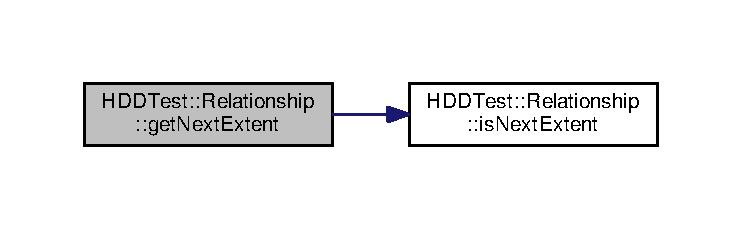
\includegraphics[width=350pt]{class_h_d_d_test_1_1_relationship_a4056c89b36da88b193ad5121b496a191_cgraph}
\end{center}
\end{figure}




Here is the caller graph for this function\-:
\nopagebreak
\begin{figure}[H]
\begin{center}
\leavevmode
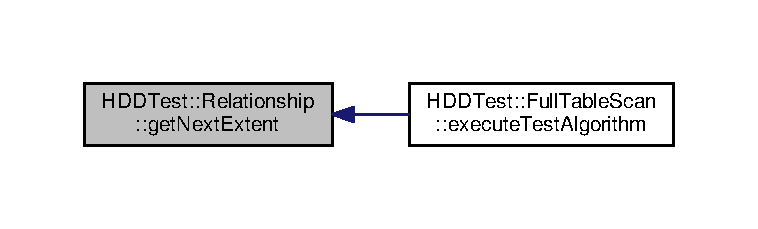
\includegraphics[width=350pt]{class_h_d_d_test_1_1_relationship_a4056c89b36da88b193ad5121b496a191_icgraph}
\end{center}
\end{figure}


\hypertarget{class_h_d_d_test_1_1_relationship_ad75f07a4f643229d0a5936746218e447}{\index{H\-D\-D\-Test\-::\-Relationship@{H\-D\-D\-Test\-::\-Relationship}!get\-Next\-Page@{get\-Next\-Page}}
\index{get\-Next\-Page@{get\-Next\-Page}!HDDTest::Relationship@{H\-D\-D\-Test\-::\-Relationship}}
\subsubsection[{get\-Next\-Page}]{\setlength{\rightskip}{0pt plus 5cm}unsigned long long int H\-D\-D\-Test\-::\-Relationship\-::get\-Next\-Page (
\begin{DoxyParamCaption}
{}
\end{DoxyParamCaption}
)}}\label{class_h_d_d_test_1_1_relationship_ad75f07a4f643229d0a5936746218e447}
\hypertarget{class_h_d_d_test_1_1_relationship_aaa19b28455227ef6d859d55f7a789f37}{\index{H\-D\-D\-Test\-::\-Relationship@{H\-D\-D\-Test\-::\-Relationship}!get\-Probability@{get\-Probability}}
\index{get\-Probability@{get\-Probability}!HDDTest::Relationship@{H\-D\-D\-Test\-::\-Relationship}}
\subsubsection[{get\-Probability}]{\setlength{\rightskip}{0pt plus 5cm}int H\-D\-D\-Test\-::\-Relationship\-::get\-Probability (
\begin{DoxyParamCaption}
\item[{unsigned long long int}]{total\-Unallocated\-Extents}
\end{DoxyParamCaption}
)}}\label{class_h_d_d_test_1_1_relationship_aaa19b28455227ef6d859d55f7a789f37}


Definition at line 57 of file Relationship.\-cpp.

\hypertarget{class_h_d_d_test_1_1_relationship_aab85efd51398e63d39757f6687eb0ecb}{\index{H\-D\-D\-Test\-::\-Relationship@{H\-D\-D\-Test\-::\-Relationship}!get\-Random\-Extent@{get\-Random\-Extent}}
\index{get\-Random\-Extent@{get\-Random\-Extent}!HDDTest::Relationship@{H\-D\-D\-Test\-::\-Relationship}}
\subsubsection[{get\-Random\-Extent}]{\setlength{\rightskip}{0pt plus 5cm}unsigned long long int H\-D\-D\-Test\-::\-Relationship\-::get\-Random\-Extent (
\begin{DoxyParamCaption}
{}
\end{DoxyParamCaption}
)}}\label{class_h_d_d_test_1_1_relationship_aab85efd51398e63d39757f6687eb0ecb}


Definition at line 63 of file Relationship.\-cpp.

\hypertarget{class_h_d_d_test_1_1_relationship_a74ccc8382a49d15d4ddd3673edef1ccc}{\index{H\-D\-D\-Test\-::\-Relationship@{H\-D\-D\-Test\-::\-Relationship}!get\-Random\-Page@{get\-Random\-Page}}
\index{get\-Random\-Page@{get\-Random\-Page}!HDDTest::Relationship@{H\-D\-D\-Test\-::\-Relationship}}
\subsubsection[{get\-Random\-Page}]{\setlength{\rightskip}{0pt plus 5cm}unsigned long long int H\-D\-D\-Test\-::\-Relationship\-::get\-Random\-Page (
\begin{DoxyParamCaption}
{}
\end{DoxyParamCaption}
)}}\label{class_h_d_d_test_1_1_relationship_a74ccc8382a49d15d4ddd3673edef1ccc}


Definition at line 68 of file Relationship.\-cpp.



Here is the caller graph for this function\-:
\nopagebreak
\begin{figure}[H]
\begin{center}
\leavevmode
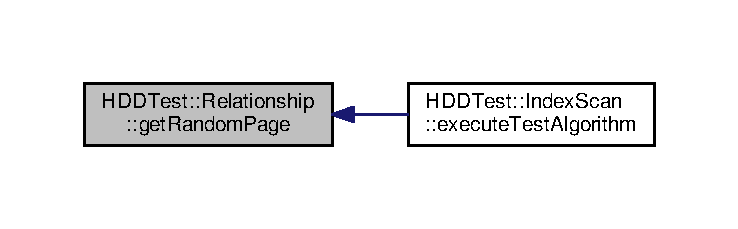
\includegraphics[width=350pt]{class_h_d_d_test_1_1_relationship_a74ccc8382a49d15d4ddd3673edef1ccc_icgraph}
\end{center}
\end{figure}


\hypertarget{class_h_d_d_test_1_1_relationship_a53966cb62025f69c97a18919e83b98c0}{\index{H\-D\-D\-Test\-::\-Relationship@{H\-D\-D\-Test\-::\-Relationship}!is\-Next\-Extent@{is\-Next\-Extent}}
\index{is\-Next\-Extent@{is\-Next\-Extent}!HDDTest::Relationship@{H\-D\-D\-Test\-::\-Relationship}}
\subsubsection[{is\-Next\-Extent}]{\setlength{\rightskip}{0pt plus 5cm}bool H\-D\-D\-Test\-::\-Relationship\-::is\-Next\-Extent (
\begin{DoxyParamCaption}
{}
\end{DoxyParamCaption}
)}}\label{class_h_d_d_test_1_1_relationship_a53966cb62025f69c97a18919e83b98c0}


Definition at line 52 of file Relationship.\-cpp.



Here is the caller graph for this function\-:
\nopagebreak
\begin{figure}[H]
\begin{center}
\leavevmode
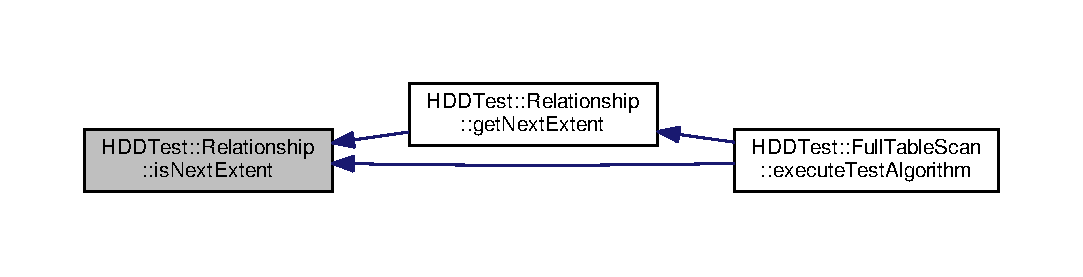
\includegraphics[width=350pt]{class_h_d_d_test_1_1_relationship_a53966cb62025f69c97a18919e83b98c0_icgraph}
\end{center}
\end{figure}


\hypertarget{class_h_d_d_test_1_1_relationship_a56e5c53a0f3cb8ea86b18aef057ea61a}{\index{H\-D\-D\-Test\-::\-Relationship@{H\-D\-D\-Test\-::\-Relationship}!set\-Unallocated\-Extents@{set\-Unallocated\-Extents}}
\index{set\-Unallocated\-Extents@{set\-Unallocated\-Extents}!HDDTest::Relationship@{H\-D\-D\-Test\-::\-Relationship}}
\subsubsection[{set\-Unallocated\-Extents}]{\setlength{\rightskip}{0pt plus 5cm}void H\-D\-D\-Test\-::\-Relationship\-::set\-Unallocated\-Extents (
\begin{DoxyParamCaption}
\item[{unsigned long long int}]{unallocated\-Extents}
\end{DoxyParamCaption}
)\hspace{0.3cm}{\ttfamily [inline]}}}\label{class_h_d_d_test_1_1_relationship_a56e5c53a0f3cb8ea86b18aef057ea61a}


Definition at line 30 of file Relationship.\-h.



\subsection{Member Data Documentation}
\hypertarget{class_h_d_d_test_1_1_relationship_a06c160bdbec302af0040fbbadd368c70}{\index{H\-D\-D\-Test\-::\-Relationship@{H\-D\-D\-Test\-::\-Relationship}!extents@{extents}}
\index{extents@{extents}!HDDTest::Relationship@{H\-D\-D\-Test\-::\-Relationship}}
\subsubsection[{extents}]{\setlength{\rightskip}{0pt plus 5cm}std\-::vector$<$struct {\bf Extent}$>$ H\-D\-D\-Test\-::\-Relationship\-::extents}}\label{class_h_d_d_test_1_1_relationship_a06c160bdbec302af0040fbbadd368c70}


Definition at line 43 of file Relationship.\-h.

\hypertarget{class_h_d_d_test_1_1_relationship_a3de1cc2d49400d4914d958a0ca17f672}{\index{H\-D\-D\-Test\-::\-Relationship@{H\-D\-D\-Test\-::\-Relationship}!name@{name}}
\index{name@{name}!HDDTest::Relationship@{H\-D\-D\-Test\-::\-Relationship}}
\subsubsection[{name}]{\setlength{\rightskip}{0pt plus 5cm}std\-::string H\-D\-D\-Test\-::\-Relationship\-::name}}\label{class_h_d_d_test_1_1_relationship_a3de1cc2d49400d4914d958a0ca17f672}


Definition at line 44 of file Relationship.\-h.

\hypertarget{class_h_d_d_test_1_1_relationship_ac986788af3ce964e514a737645aa6cd1}{\index{H\-D\-D\-Test\-::\-Relationship@{H\-D\-D\-Test\-::\-Relationship}!page\-Size\-In\-K\-B@{page\-Size\-In\-K\-B}}
\index{page\-Size\-In\-K\-B@{page\-Size\-In\-K\-B}!HDDTest::Relationship@{H\-D\-D\-Test\-::\-Relationship}}
\subsubsection[{page\-Size\-In\-K\-B}]{\setlength{\rightskip}{0pt plus 5cm}unsigned int H\-D\-D\-Test\-::\-Relationship\-::page\-Size\-In\-K\-B}}\label{class_h_d_d_test_1_1_relationship_ac986788af3ce964e514a737645aa6cd1}


Definition at line 47 of file Relationship.\-h.

\hypertarget{class_h_d_d_test_1_1_relationship_ada41b15d153b3baa5788de2a66295bcb}{\index{H\-D\-D\-Test\-::\-Relationship@{H\-D\-D\-Test\-::\-Relationship}!pages\-Per\-Extent@{pages\-Per\-Extent}}
\index{pages\-Per\-Extent@{pages\-Per\-Extent}!HDDTest::Relationship@{H\-D\-D\-Test\-::\-Relationship}}
\subsubsection[{pages\-Per\-Extent}]{\setlength{\rightskip}{0pt plus 5cm}unsigned int H\-D\-D\-Test\-::\-Relationship\-::pages\-Per\-Extent}}\label{class_h_d_d_test_1_1_relationship_ada41b15d153b3baa5788de2a66295bcb}


Definition at line 46 of file Relationship.\-h.



The documentation for this class was generated from the following files\-:\begin{DoxyCompactItemize}
\item 
src/\-Layout/\hyperlink{_relationship_8h}{Relationship.\-h}\item 
src/\-Layout/\hyperlink{_relationship_8cpp}{Relationship.\-cpp}\end{DoxyCompactItemize}

\hypertarget{struct_h_d_d_test_1_1_relationship_config}{\section{H\-D\-D\-Test\-:\-:Relationship\-Config Struct Reference}
\label{struct_h_d_d_test_1_1_relationship_config}\index{H\-D\-D\-Test\-::\-Relationship\-Config@{H\-D\-D\-Test\-::\-Relationship\-Config}}
}


{\ttfamily \#include $<$Layout.\-h$>$}

\subsection*{Public Attributes}
\begin{DoxyCompactItemize}
\item 
unsigned int \hyperlink{struct_h_d_d_test_1_1_relationship_config_aa85591a1ae2dce1683ea483f410d281d}{size}
\item 
std\-::string \hyperlink{struct_h_d_d_test_1_1_relationship_config_afd83c7f8b3b77c39814f43e1e86c56c8}{name}
\end{DoxyCompactItemize}


\subsection{Detailed Description}


Definition at line 18 of file Layout.\-h.



\subsection{Member Data Documentation}
\hypertarget{struct_h_d_d_test_1_1_relationship_config_afd83c7f8b3b77c39814f43e1e86c56c8}{\index{H\-D\-D\-Test\-::\-Relationship\-Config@{H\-D\-D\-Test\-::\-Relationship\-Config}!name@{name}}
\index{name@{name}!HDDTest::RelationshipConfig@{H\-D\-D\-Test\-::\-Relationship\-Config}}
\subsubsection[{name}]{\setlength{\rightskip}{0pt plus 5cm}std\-::string H\-D\-D\-Test\-::\-Relationship\-Config\-::name}}\label{struct_h_d_d_test_1_1_relationship_config_afd83c7f8b3b77c39814f43e1e86c56c8}


Definition at line 21 of file Layout.\-h.

\hypertarget{struct_h_d_d_test_1_1_relationship_config_aa85591a1ae2dce1683ea483f410d281d}{\index{H\-D\-D\-Test\-::\-Relationship\-Config@{H\-D\-D\-Test\-::\-Relationship\-Config}!size@{size}}
\index{size@{size}!HDDTest::RelationshipConfig@{H\-D\-D\-Test\-::\-Relationship\-Config}}
\subsubsection[{size}]{\setlength{\rightskip}{0pt plus 5cm}unsigned int H\-D\-D\-Test\-::\-Relationship\-Config\-::size}}\label{struct_h_d_d_test_1_1_relationship_config_aa85591a1ae2dce1683ea483f410d281d}


Definition at line 20 of file Layout.\-h.



The documentation for this struct was generated from the following file\-:\begin{DoxyCompactItemize}
\item 
src/\-Layout/\hyperlink{_layout_8h}{Layout.\-h}\end{DoxyCompactItemize}

\hypertarget{class_h_d_d_test_1_1_test_scenario}{\section{H\-D\-D\-Test\-:\-:Test\-Scenario Class Reference}
\label{class_h_d_d_test_1_1_test_scenario}\index{H\-D\-D\-Test\-::\-Test\-Scenario@{H\-D\-D\-Test\-::\-Test\-Scenario}}
}


{\ttfamily \#include $<$Test\-Scenario.\-h$>$}

\subsection*{Public Member Functions}
\begin{DoxyCompactItemize}
\item 
\hyperlink{class_h_d_d_test_1_1_test_scenario_abbe9499202d1095c50140f570a2532dc}{Test\-Scenario} (std\-::string, std\-::vector$<$ std\-::string $>$ $\ast$, std\-::unordered\-\_\-map$<$ std\-::string, \hyperlink{class_h_d_d_test_1_1_layout}{Layout} $\ast$ $>$ $\ast$, \hyperlink{struct_h_d_d_test_1_1_test_settings}{Test\-Settings}, std\-::vector$<$ \hyperlink{struct_h_d_d_test_1_1_test_settings}{Test\-Settings} $>$)
\item 
virtual \hyperlink{class_h_d_d_test_1_1_test_scenario_a696957520e2865654b1a3fb862c386c0}{$\sim$\-Test\-Scenario} ()
\item 
void \hyperlink{class_h_d_d_test_1_1_test_scenario_a33ace13f97b5c5ded8da22ca55416c5a}{run} ()
\item 
int \hyperlink{class_h_d_d_test_1_1_test_scenario_afe92bd2a756f3f753f7cb8e8dd59eb53}{get\-Number\-Of\-Tests} ()
\end{DoxyCompactItemize}


\subsection{Detailed Description}


Definition at line 19 of file Test\-Scenario.\-h.



\subsection{Constructor \& Destructor Documentation}
\hypertarget{class_h_d_d_test_1_1_test_scenario_abbe9499202d1095c50140f570a2532dc}{\index{H\-D\-D\-Test\-::\-Test\-Scenario@{H\-D\-D\-Test\-::\-Test\-Scenario}!Test\-Scenario@{Test\-Scenario}}
\index{Test\-Scenario@{Test\-Scenario}!HDDTest::TestScenario@{H\-D\-D\-Test\-::\-Test\-Scenario}}
\subsubsection[{Test\-Scenario}]{\setlength{\rightskip}{0pt plus 5cm}H\-D\-D\-Test\-::\-Test\-Scenario\-::\-Test\-Scenario (
\begin{DoxyParamCaption}
\item[{std\-::string}]{name, }
\item[{std\-::vector$<$ std\-::string $>$ $\ast$}]{disk\-Paths, }
\item[{std\-::unordered\-\_\-map$<$ std\-::string, {\bf Layout} $\ast$ $>$ $\ast$}]{layouts, }
\item[{{\bf Test\-Settings}}]{main\-Thread\-Settings, }
\item[{std\-::vector$<$ {\bf Test\-Settings} $>$}]{background\-Threads\-Settings}
\end{DoxyParamCaption}
)}}\label{class_h_d_d_test_1_1_test_scenario_abbe9499202d1095c50140f570a2532dc}


Definition at line 15 of file Test\-Scenario.\-cpp.

\hypertarget{class_h_d_d_test_1_1_test_scenario_a696957520e2865654b1a3fb862c386c0}{\index{H\-D\-D\-Test\-::\-Test\-Scenario@{H\-D\-D\-Test\-::\-Test\-Scenario}!$\sim$\-Test\-Scenario@{$\sim$\-Test\-Scenario}}
\index{$\sim$\-Test\-Scenario@{$\sim$\-Test\-Scenario}!HDDTest::TestScenario@{H\-D\-D\-Test\-::\-Test\-Scenario}}
\subsubsection[{$\sim$\-Test\-Scenario}]{\setlength{\rightskip}{0pt plus 5cm}H\-D\-D\-Test\-::\-Test\-Scenario\-::$\sim$\-Test\-Scenario (
\begin{DoxyParamCaption}
{}
\end{DoxyParamCaption}
)\hspace{0.3cm}{\ttfamily [virtual]}}}\label{class_h_d_d_test_1_1_test_scenario_a696957520e2865654b1a3fb862c386c0}


Definition at line 24 of file Test\-Scenario.\-cpp.



\subsection{Member Function Documentation}
\hypertarget{class_h_d_d_test_1_1_test_scenario_afe92bd2a756f3f753f7cb8e8dd59eb53}{\index{H\-D\-D\-Test\-::\-Test\-Scenario@{H\-D\-D\-Test\-::\-Test\-Scenario}!get\-Number\-Of\-Tests@{get\-Number\-Of\-Tests}}
\index{get\-Number\-Of\-Tests@{get\-Number\-Of\-Tests}!HDDTest::TestScenario@{H\-D\-D\-Test\-::\-Test\-Scenario}}
\subsubsection[{get\-Number\-Of\-Tests}]{\setlength{\rightskip}{0pt plus 5cm}int H\-D\-D\-Test\-::\-Test\-Scenario\-::get\-Number\-Of\-Tests (
\begin{DoxyParamCaption}
{}
\end{DoxyParamCaption}
)}}\label{class_h_d_d_test_1_1_test_scenario_afe92bd2a756f3f753f7cb8e8dd59eb53}


Definition at line 79 of file Test\-Scenario.\-cpp.



Here is the caller graph for this function\-:\nopagebreak
\begin{figure}[H]
\begin{center}
\leavevmode
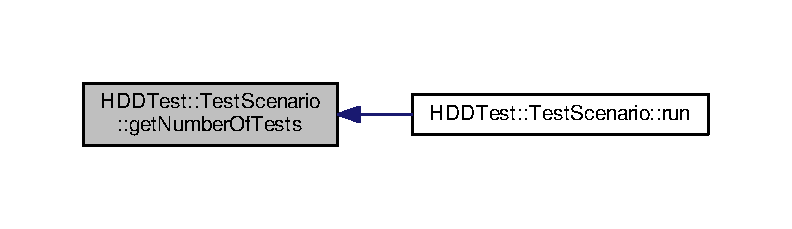
\includegraphics[width=350pt]{class_h_d_d_test_1_1_test_scenario_afe92bd2a756f3f753f7cb8e8dd59eb53_icgraph}
\end{center}
\end{figure}


\hypertarget{class_h_d_d_test_1_1_test_scenario_a33ace13f97b5c5ded8da22ca55416c5a}{\index{H\-D\-D\-Test\-::\-Test\-Scenario@{H\-D\-D\-Test\-::\-Test\-Scenario}!run@{run}}
\index{run@{run}!HDDTest::TestScenario@{H\-D\-D\-Test\-::\-Test\-Scenario}}
\subsubsection[{run}]{\setlength{\rightskip}{0pt plus 5cm}void H\-D\-D\-Test\-::\-Test\-Scenario\-::run (
\begin{DoxyParamCaption}
{}
\end{DoxyParamCaption}
)}}\label{class_h_d_d_test_1_1_test_scenario_a33ace13f97b5c5ded8da22ca55416c5a}


Definition at line 30 of file Test\-Scenario.\-cpp.



Here is the call graph for this function\-:
\nopagebreak
\begin{figure}[H]
\begin{center}
\leavevmode
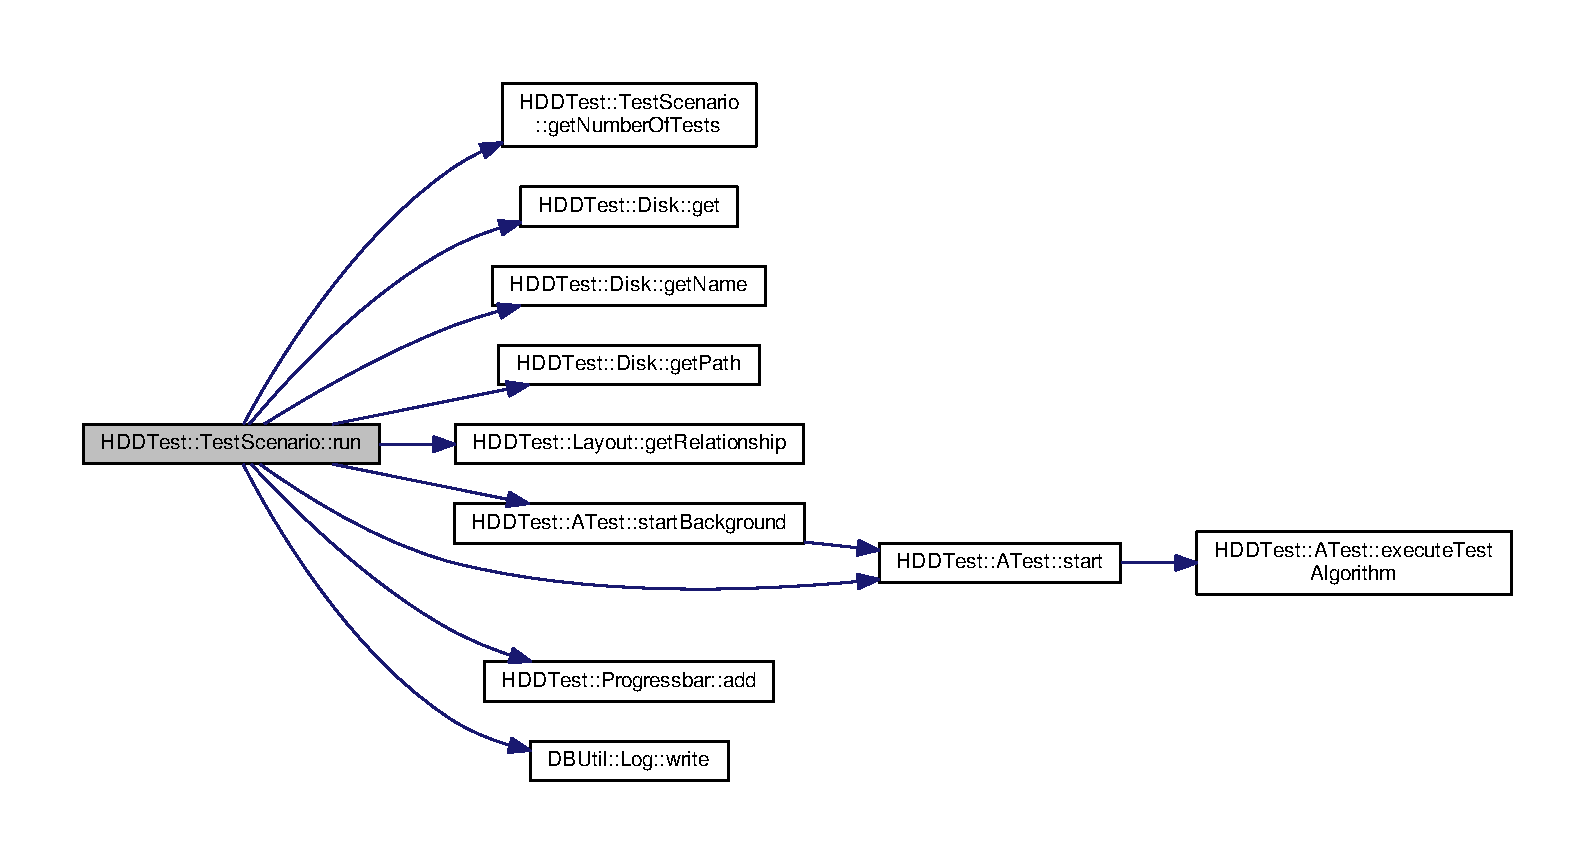
\includegraphics[width=350pt]{class_h_d_d_test_1_1_test_scenario_a33ace13f97b5c5ded8da22ca55416c5a_cgraph}
\end{center}
\end{figure}




The documentation for this class was generated from the following files\-:\begin{DoxyCompactItemize}
\item 
src/\-Tests/\hyperlink{_test_scenario_8h}{Test\-Scenario.\-h}\item 
src/\-Tests/\hyperlink{_test_scenario_8cpp}{Test\-Scenario.\-cpp}\end{DoxyCompactItemize}

\hypertarget{struct_h_d_d_test_1_1_test_settings}{\section{H\-D\-D\-Test\-:\-:Test\-Settings Struct Reference}
\label{struct_h_d_d_test_1_1_test_settings}\index{H\-D\-D\-Test\-::\-Test\-Settings@{H\-D\-D\-Test\-::\-Test\-Settings}}
}


{\ttfamily \#include $<$A\-Test.\-h$>$}

\subsection*{Public Attributes}
\begin{DoxyCompactItemize}
\item 
std\-::string \hyperlink{struct_h_d_d_test_1_1_test_settings_acb1acd81644b7dc295e3cfd187469cb9}{name}
\item 
std\-::uint64\-\_\-t \hyperlink{struct_h_d_d_test_1_1_test_settings_a689e6ed46e39f14544a7f257c506d9b9}{sleep}
\item 
std\-::string \hyperlink{struct_h_d_d_test_1_1_test_settings_a2ae4bf77f3d9d63cc28ac44622327d23}{relationship}
\end{DoxyCompactItemize}


\subsection{Detailed Description}


Definition at line 19 of file A\-Test.\-h.



\subsection{Member Data Documentation}
\hypertarget{struct_h_d_d_test_1_1_test_settings_acb1acd81644b7dc295e3cfd187469cb9}{\index{H\-D\-D\-Test\-::\-Test\-Settings@{H\-D\-D\-Test\-::\-Test\-Settings}!name@{name}}
\index{name@{name}!HDDTest::TestSettings@{H\-D\-D\-Test\-::\-Test\-Settings}}
\subsubsection[{name}]{\setlength{\rightskip}{0pt plus 5cm}std\-::string H\-D\-D\-Test\-::\-Test\-Settings\-::name}}\label{struct_h_d_d_test_1_1_test_settings_acb1acd81644b7dc295e3cfd187469cb9}


Definition at line 21 of file A\-Test.\-h.

\hypertarget{struct_h_d_d_test_1_1_test_settings_a2ae4bf77f3d9d63cc28ac44622327d23}{\index{H\-D\-D\-Test\-::\-Test\-Settings@{H\-D\-D\-Test\-::\-Test\-Settings}!relationship@{relationship}}
\index{relationship@{relationship}!HDDTest::TestSettings@{H\-D\-D\-Test\-::\-Test\-Settings}}
\subsubsection[{relationship}]{\setlength{\rightskip}{0pt plus 5cm}std\-::string H\-D\-D\-Test\-::\-Test\-Settings\-::relationship}}\label{struct_h_d_d_test_1_1_test_settings_a2ae4bf77f3d9d63cc28ac44622327d23}


Definition at line 23 of file A\-Test.\-h.

\hypertarget{struct_h_d_d_test_1_1_test_settings_a689e6ed46e39f14544a7f257c506d9b9}{\index{H\-D\-D\-Test\-::\-Test\-Settings@{H\-D\-D\-Test\-::\-Test\-Settings}!sleep@{sleep}}
\index{sleep@{sleep}!HDDTest::TestSettings@{H\-D\-D\-Test\-::\-Test\-Settings}}
\subsubsection[{sleep}]{\setlength{\rightskip}{0pt plus 5cm}std\-::uint64\-\_\-t H\-D\-D\-Test\-::\-Test\-Settings\-::sleep}}\label{struct_h_d_d_test_1_1_test_settings_a689e6ed46e39f14544a7f257c506d9b9}


Definition at line 22 of file A\-Test.\-h.



The documentation for this struct was generated from the following file\-:\begin{DoxyCompactItemize}
\item 
src/\-Tests/\hyperlink{_a_test_8h}{A\-Test.\-h}\end{DoxyCompactItemize}

\hypertarget{class_h_d_d_test_1_1_transaction_log}{\section{H\-D\-D\-Test\-:\-:Transaction\-Log Class Reference}
\label{class_h_d_d_test_1_1_transaction_log}\index{H\-D\-D\-Test\-::\-Transaction\-Log@{H\-D\-D\-Test\-::\-Transaction\-Log}}
}


{\ttfamily \#include $<$Transaction\-Log.\-h$>$}



Inheritance diagram for H\-D\-D\-Test\-:\-:Transaction\-Log\-:
\nopagebreak
\begin{figure}[H]
\begin{center}
\leavevmode
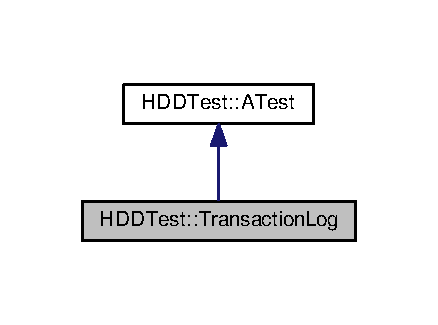
\includegraphics[width=210pt]{class_h_d_d_test_1_1_transaction_log__inherit__graph}
\end{center}
\end{figure}


Collaboration diagram for H\-D\-D\-Test\-:\-:Transaction\-Log\-:
\nopagebreak
\begin{figure}[H]
\begin{center}
\leavevmode
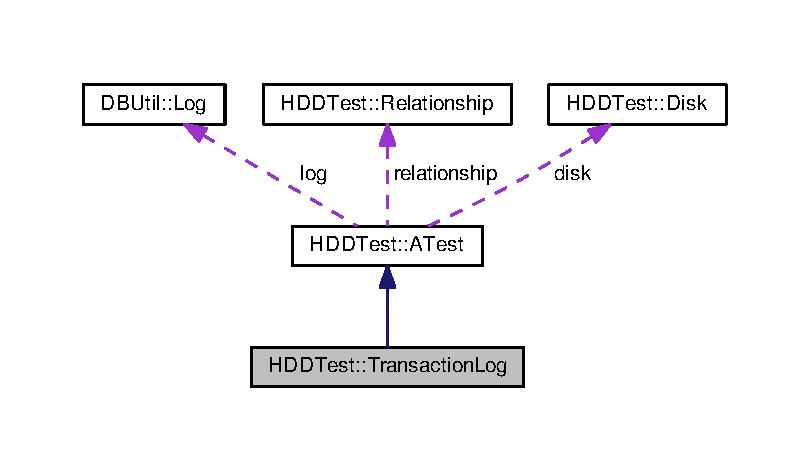
\includegraphics[width=350pt]{class_h_d_d_test_1_1_transaction_log__coll__graph}
\end{center}
\end{figure}
\subsection*{Public Member Functions}
\begin{DoxyCompactItemize}
\item 
\hyperlink{class_h_d_d_test_1_1_transaction_log_ab6c72f23eff8b91c3dc71727480ba0fa}{Transaction\-Log} (std\-::string, \hyperlink{class_h_d_d_test_1_1_disk}{Disk} $\ast$, \hyperlink{class_h_d_d_test_1_1_relationship}{Relationship} $\ast$)
\item 
virtual \hyperlink{class_h_d_d_test_1_1_transaction_log_a0ff191553e0eb906cec8964daf57730e}{$\sim$\-Transaction\-Log} ()
\item 
void \hyperlink{class_h_d_d_test_1_1_transaction_log_a3454c7970a87effe1f5154e7bcd73273}{execute\-Test\-Algorithm} () override
\end{DoxyCompactItemize}
\subsection*{Additional Inherited Members}


\subsection{Detailed Description}


Definition at line 14 of file Transaction\-Log.\-h.



\subsection{Constructor \& Destructor Documentation}
\hypertarget{class_h_d_d_test_1_1_transaction_log_ab6c72f23eff8b91c3dc71727480ba0fa}{\index{H\-D\-D\-Test\-::\-Transaction\-Log@{H\-D\-D\-Test\-::\-Transaction\-Log}!Transaction\-Log@{Transaction\-Log}}
\index{Transaction\-Log@{Transaction\-Log}!HDDTest::TransactionLog@{H\-D\-D\-Test\-::\-Transaction\-Log}}
\subsubsection[{Transaction\-Log}]{\setlength{\rightskip}{0pt plus 5cm}H\-D\-D\-Test\-::\-Transaction\-Log\-::\-Transaction\-Log (
\begin{DoxyParamCaption}
\item[{std\-::string}]{name, }
\item[{{\bf Disk} $\ast$}]{disk, }
\item[{{\bf Relationship} $\ast$}]{relationship}
\end{DoxyParamCaption}
)}}\label{class_h_d_d_test_1_1_transaction_log_ab6c72f23eff8b91c3dc71727480ba0fa}


Definition at line 12 of file Transaction\-Log.\-cpp.



Here is the call graph for this function\-:
\nopagebreak
\begin{figure}[H]
\begin{center}
\leavevmode
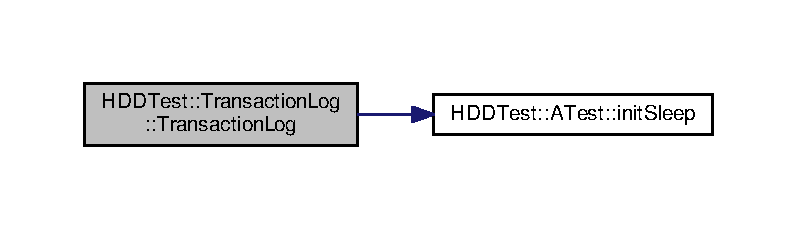
\includegraphics[width=350pt]{class_h_d_d_test_1_1_transaction_log_ab6c72f23eff8b91c3dc71727480ba0fa_cgraph}
\end{center}
\end{figure}


\hypertarget{class_h_d_d_test_1_1_transaction_log_a0ff191553e0eb906cec8964daf57730e}{\index{H\-D\-D\-Test\-::\-Transaction\-Log@{H\-D\-D\-Test\-::\-Transaction\-Log}!$\sim$\-Transaction\-Log@{$\sim$\-Transaction\-Log}}
\index{$\sim$\-Transaction\-Log@{$\sim$\-Transaction\-Log}!HDDTest::TransactionLog@{H\-D\-D\-Test\-::\-Transaction\-Log}}
\subsubsection[{$\sim$\-Transaction\-Log}]{\setlength{\rightskip}{0pt plus 5cm}H\-D\-D\-Test\-::\-Transaction\-Log\-::$\sim$\-Transaction\-Log (
\begin{DoxyParamCaption}
{}
\end{DoxyParamCaption}
)\hspace{0.3cm}{\ttfamily [virtual]}}}\label{class_h_d_d_test_1_1_transaction_log_a0ff191553e0eb906cec8964daf57730e}


Definition at line 17 of file Transaction\-Log.\-cpp.



\subsection{Member Function Documentation}
\hypertarget{class_h_d_d_test_1_1_transaction_log_a3454c7970a87effe1f5154e7bcd73273}{\index{H\-D\-D\-Test\-::\-Transaction\-Log@{H\-D\-D\-Test\-::\-Transaction\-Log}!execute\-Test\-Algorithm@{execute\-Test\-Algorithm}}
\index{execute\-Test\-Algorithm@{execute\-Test\-Algorithm}!HDDTest::TransactionLog@{H\-D\-D\-Test\-::\-Transaction\-Log}}
\subsubsection[{execute\-Test\-Algorithm}]{\setlength{\rightskip}{0pt plus 5cm}void H\-D\-D\-Test\-::\-Transaction\-Log\-::execute\-Test\-Algorithm (
\begin{DoxyParamCaption}
{}
\end{DoxyParamCaption}
)\hspace{0.3cm}{\ttfamily [override]}, {\ttfamily [virtual]}}}\label{class_h_d_d_test_1_1_transaction_log_a3454c7970a87effe1f5154e7bcd73273}


Reimplemented from \hyperlink{class_h_d_d_test_1_1_a_test_a7dc054e211eccf42c03a6bb31d7fdc6e}{H\-D\-D\-Test\-::\-A\-Test}.



Definition at line 21 of file Transaction\-Log.\-cpp.



Here is the call graph for this function\-:
\nopagebreak
\begin{figure}[H]
\begin{center}
\leavevmode
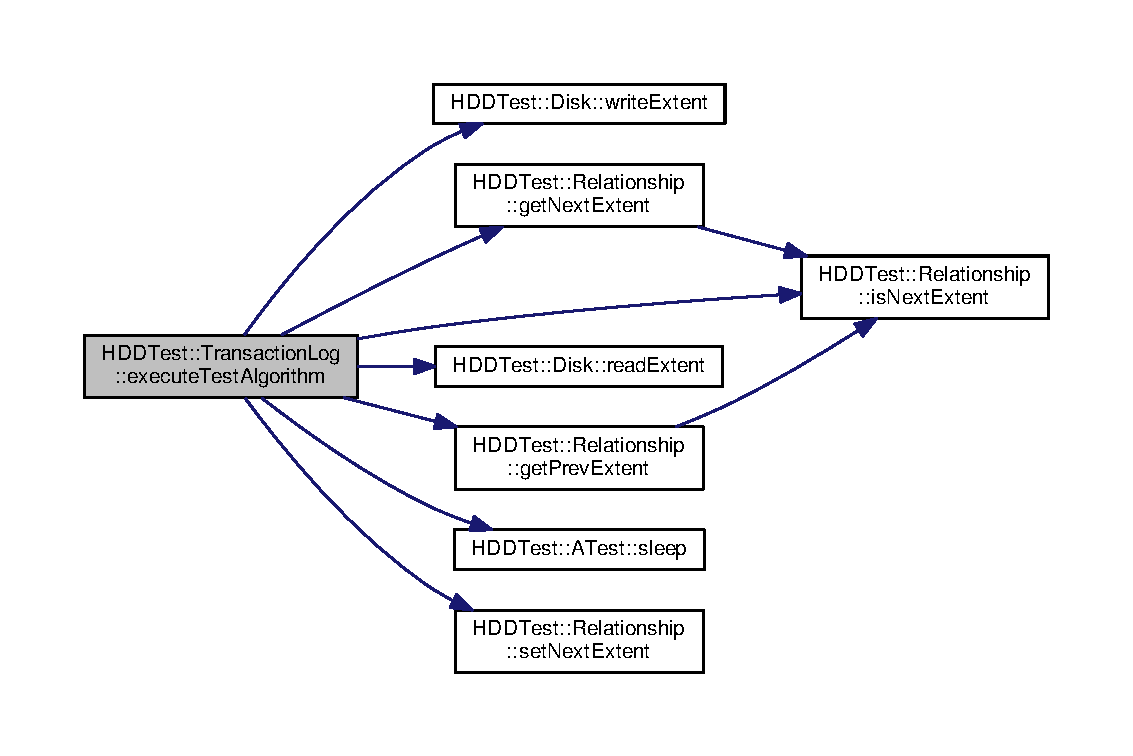
\includegraphics[width=350pt]{class_h_d_d_test_1_1_transaction_log_a3454c7970a87effe1f5154e7bcd73273_cgraph}
\end{center}
\end{figure}




The documentation for this class was generated from the following files\-:\begin{DoxyCompactItemize}
\item 
src/\-Tests/\hyperlink{_transaction_log_8h}{Transaction\-Log.\-h}\item 
src/\-Tests/\hyperlink{_transaction_log_8cpp}{Transaction\-Log.\-cpp}\end{DoxyCompactItemize}

\chapter{File Documentation}
\hypertarget{_d_b_benchmark_8cpp}{\section{src/\-D\-B\-Benchmark.cpp File Reference}
\label{_d_b_benchmark_8cpp}\index{src/\-D\-B\-Benchmark.\-cpp@{src/\-D\-B\-Benchmark.\-cpp}}
}
{\ttfamily \#include $<$iostream$>$}\\*
{\ttfamily \#include $<$unistd.\-h$>$}\\*
{\ttfamily \#include \char`\"{}Util/\-Configurator.\-h\char`\"{}}\\*
{\ttfamily \#include \char`\"{}Tests/\-Test\-Scenario.\-h\char`\"{}}\\*
Include dependency graph for D\-B\-Benchmark.\-cpp\-:\nopagebreak
\begin{figure}[H]
\begin{center}
\leavevmode
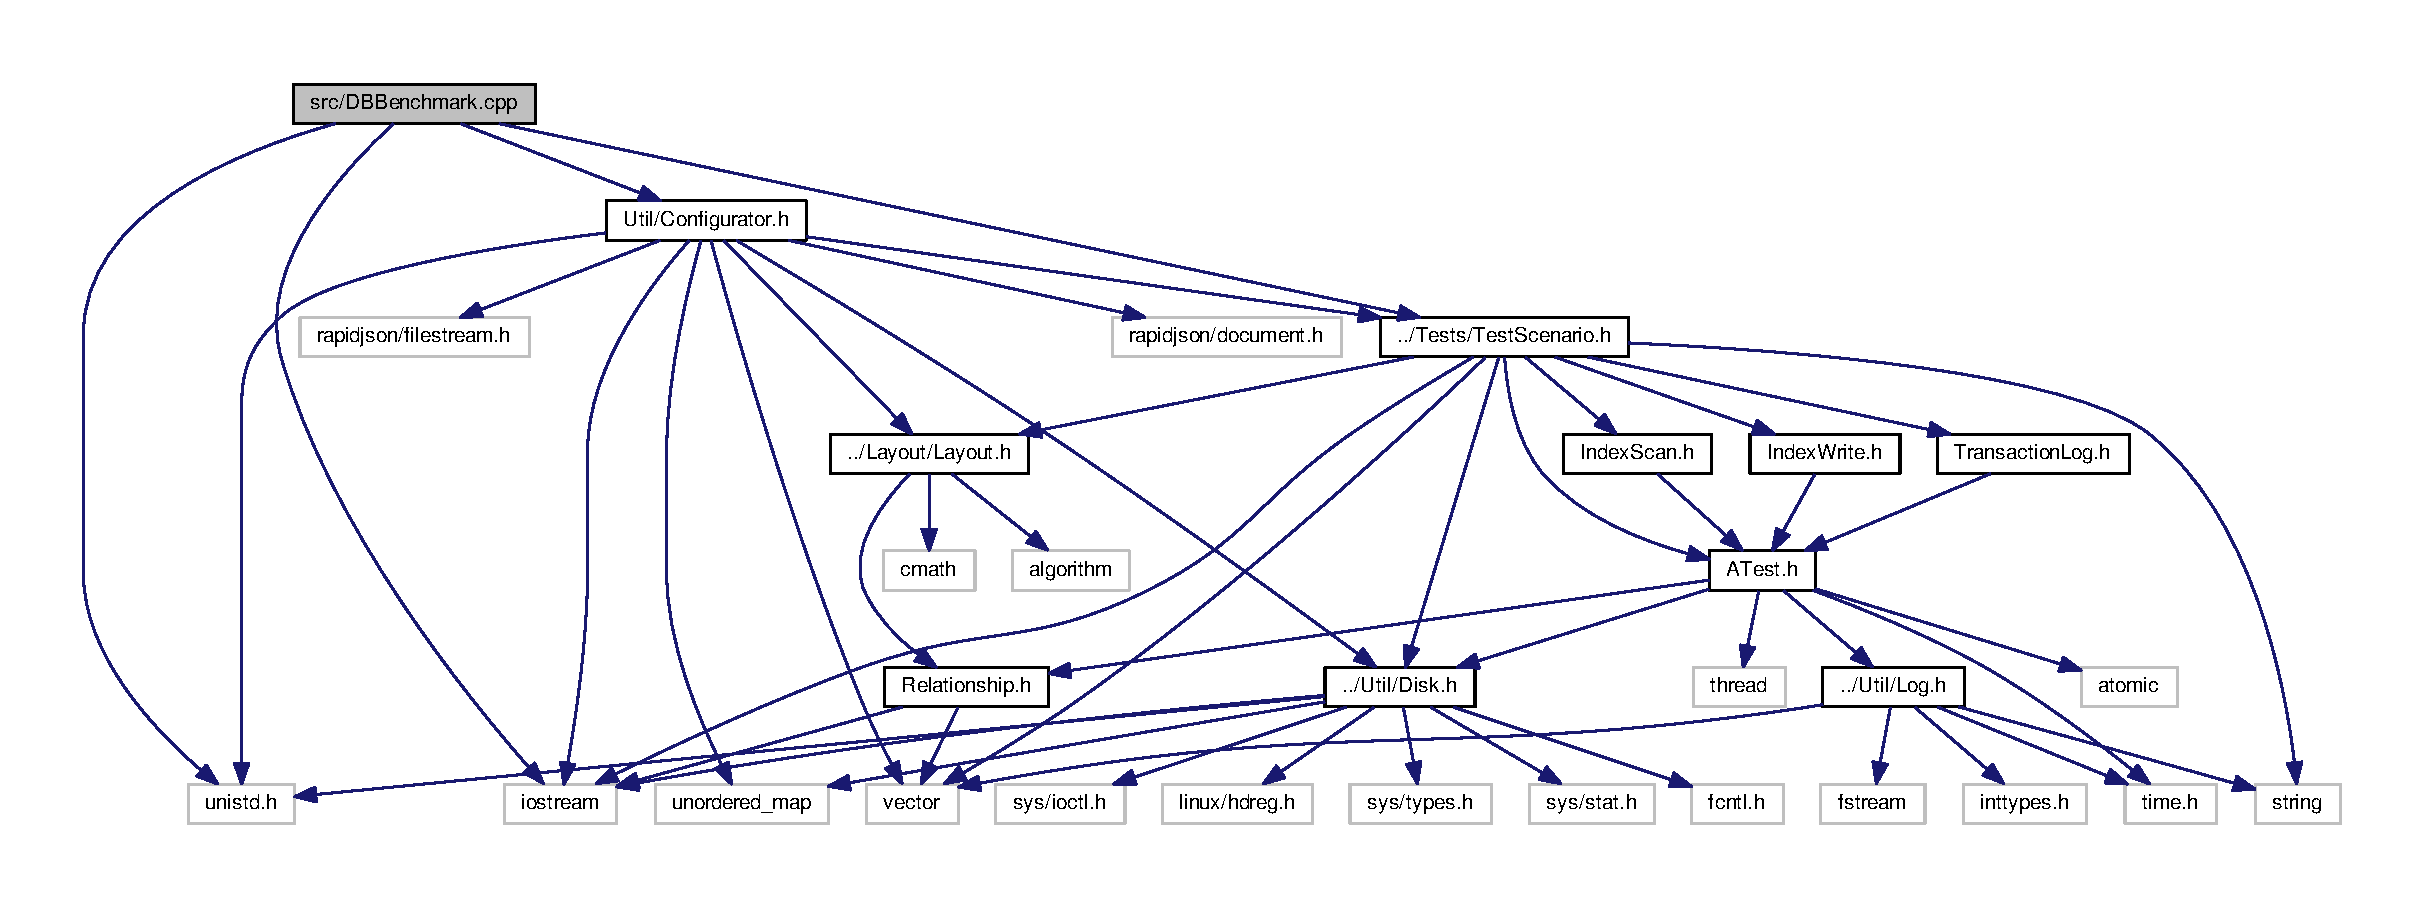
\includegraphics[width=350pt]{_d_b_benchmark_8cpp__incl}
\end{center}
\end{figure}
\subsection*{Functions}
\begin{DoxyCompactItemize}
\item 
int \hyperlink{_d_b_benchmark_8cpp_ae66f6b31b5ad750f1fe042a706a4e3d4}{main} ()
\end{DoxyCompactItemize}


\subsection{Function Documentation}
\hypertarget{_d_b_benchmark_8cpp_ae66f6b31b5ad750f1fe042a706a4e3d4}{\index{D\-B\-Benchmark.\-cpp@{D\-B\-Benchmark.\-cpp}!main@{main}}
\index{main@{main}!DBBenchmark.cpp@{D\-B\-Benchmark.\-cpp}}
\subsubsection[{main}]{\setlength{\rightskip}{0pt plus 5cm}int main (
\begin{DoxyParamCaption}
{}
\end{DoxyParamCaption}
)}}\label{_d_b_benchmark_8cpp_ae66f6b31b5ad750f1fe042a706a4e3d4}


Definition at line 13 of file D\-B\-Benchmark.\-cpp.



Here is the call graph for this function\-:
\nopagebreak
\begin{figure}[H]
\begin{center}
\leavevmode
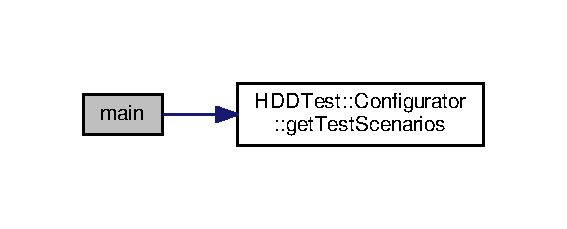
\includegraphics[width=272pt]{_d_b_benchmark_8cpp_ae66f6b31b5ad750f1fe042a706a4e3d4_cgraph}
\end{center}
\end{figure}



\hypertarget{_layout_8cpp}{\section{src/\-Layout/\-Layout.cpp File Reference}
\label{_layout_8cpp}\index{src/\-Layout/\-Layout.\-cpp@{src/\-Layout/\-Layout.\-cpp}}
}
{\ttfamily \#include \char`\"{}Layout.\-h\char`\"{}}\\*
Include dependency graph for Layout.\-cpp\-:\nopagebreak
\begin{figure}[H]
\begin{center}
\leavevmode
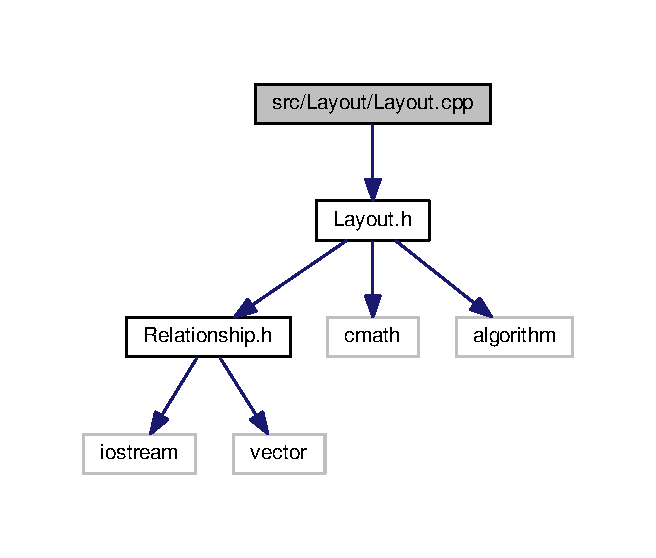
\includegraphics[width=315pt]{_layout_8cpp__incl}
\end{center}
\end{figure}
\subsection*{Namespaces}
\begin{DoxyCompactItemize}
\item 
\hyperlink{namespace_h_d_d_test}{H\-D\-D\-Test}
\end{DoxyCompactItemize}

\hypertarget{_layout_8h}{\section{src/\-Layout/\-Layout.h File Reference}
\label{_layout_8h}\index{src/\-Layout/\-Layout.\-h@{src/\-Layout/\-Layout.\-h}}
}
{\ttfamily \#include \char`\"{}Relationship.\-h\char`\"{}}\\*
{\ttfamily \#include $<$cmath$>$}\\*
{\ttfamily \#include $<$algorithm$>$}\\*
Include dependency graph for Layout.\-h\-:\nopagebreak
\begin{figure}[H]
\begin{center}
\leavevmode
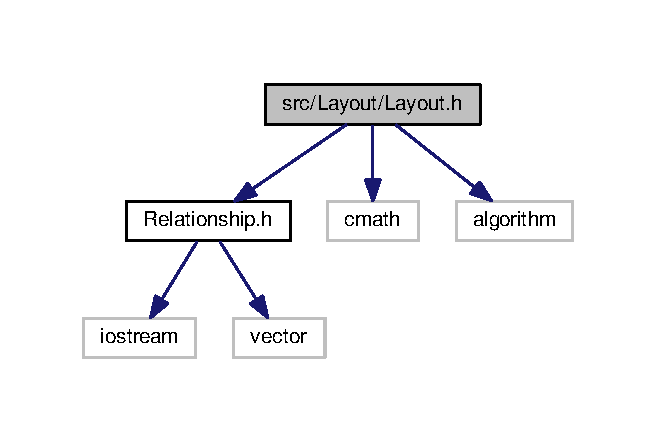
\includegraphics[width=315pt]{_layout_8h__incl}
\end{center}
\end{figure}
This graph shows which files directly or indirectly include this file\-:\nopagebreak
\begin{figure}[H]
\begin{center}
\leavevmode
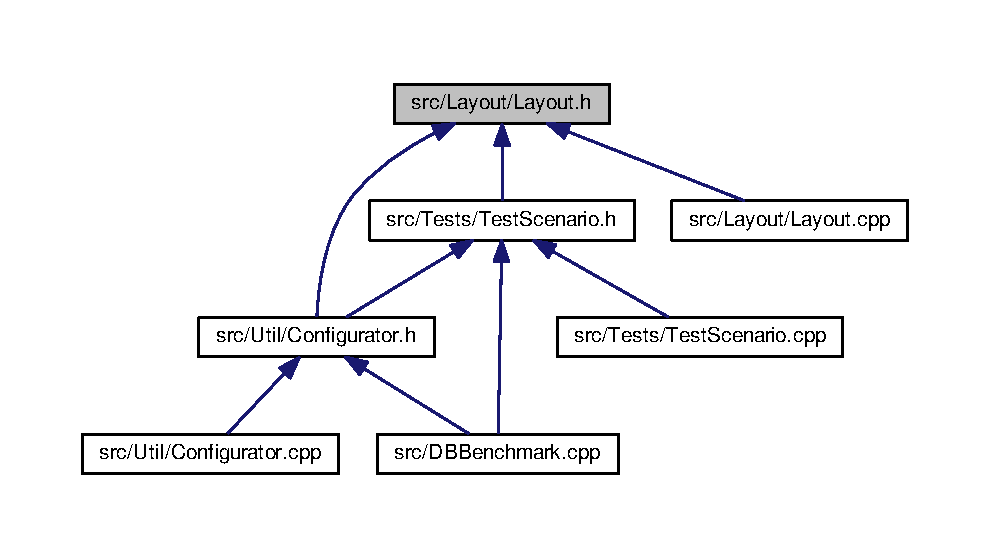
\includegraphics[width=350pt]{_layout_8h__dep__incl}
\end{center}
\end{figure}
\subsection*{Classes}
\begin{DoxyCompactItemize}
\item 
struct \hyperlink{struct_h_d_d_test_1_1_relationship_config}{H\-D\-D\-Test\-::\-Relationship\-Config}
\item 
struct \hyperlink{struct_h_d_d_test_1_1_layout_settings}{H\-D\-D\-Test\-::\-Layout\-Settings}
\item 
class \hyperlink{class_h_d_d_test_1_1_layout}{H\-D\-D\-Test\-::\-Layout}
\end{DoxyCompactItemize}
\subsection*{Namespaces}
\begin{DoxyCompactItemize}
\item 
\hyperlink{namespace_h_d_d_test}{H\-D\-D\-Test}
\end{DoxyCompactItemize}

\hypertarget{_relationship_8cpp}{\section{src/\-Layout/\-Relationship.cpp File Reference}
\label{_relationship_8cpp}\index{src/\-Layout/\-Relationship.\-cpp@{src/\-Layout/\-Relationship.\-cpp}}
}
{\ttfamily \#include \char`\"{}Relationship.\-h\char`\"{}}\\*
Include dependency graph for Relationship.\-cpp\-:
\nopagebreak
\begin{figure}[H]
\begin{center}
\leavevmode
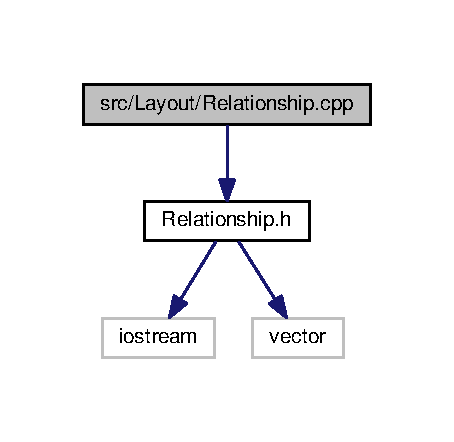
\includegraphics[width=218pt]{_relationship_8cpp__incl}
\end{center}
\end{figure}
\subsection*{Namespaces}
\begin{DoxyCompactItemize}
\item 
\hyperlink{namespace_h_d_d_test}{H\-D\-D\-Test}
\end{DoxyCompactItemize}

\hypertarget{_relationship_8h}{\section{src/\-Layout/\-Relationship.h File Reference}
\label{_relationship_8h}\index{src/\-Layout/\-Relationship.\-h@{src/\-Layout/\-Relationship.\-h}}
}
{\ttfamily \#include $<$iostream$>$}\\*
{\ttfamily \#include $<$vector$>$}\\*
Include dependency graph for Relationship.\-h\-:\nopagebreak
\begin{figure}[H]
\begin{center}
\leavevmode
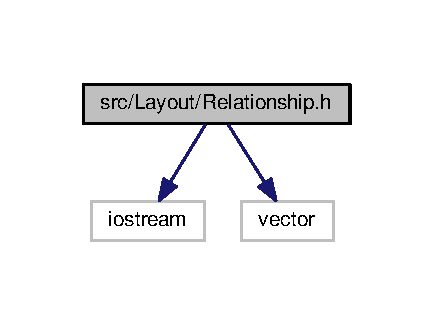
\includegraphics[width=208pt]{_relationship_8h__incl}
\end{center}
\end{figure}
This graph shows which files directly or indirectly include this file\-:
\nopagebreak
\begin{figure}[H]
\begin{center}
\leavevmode
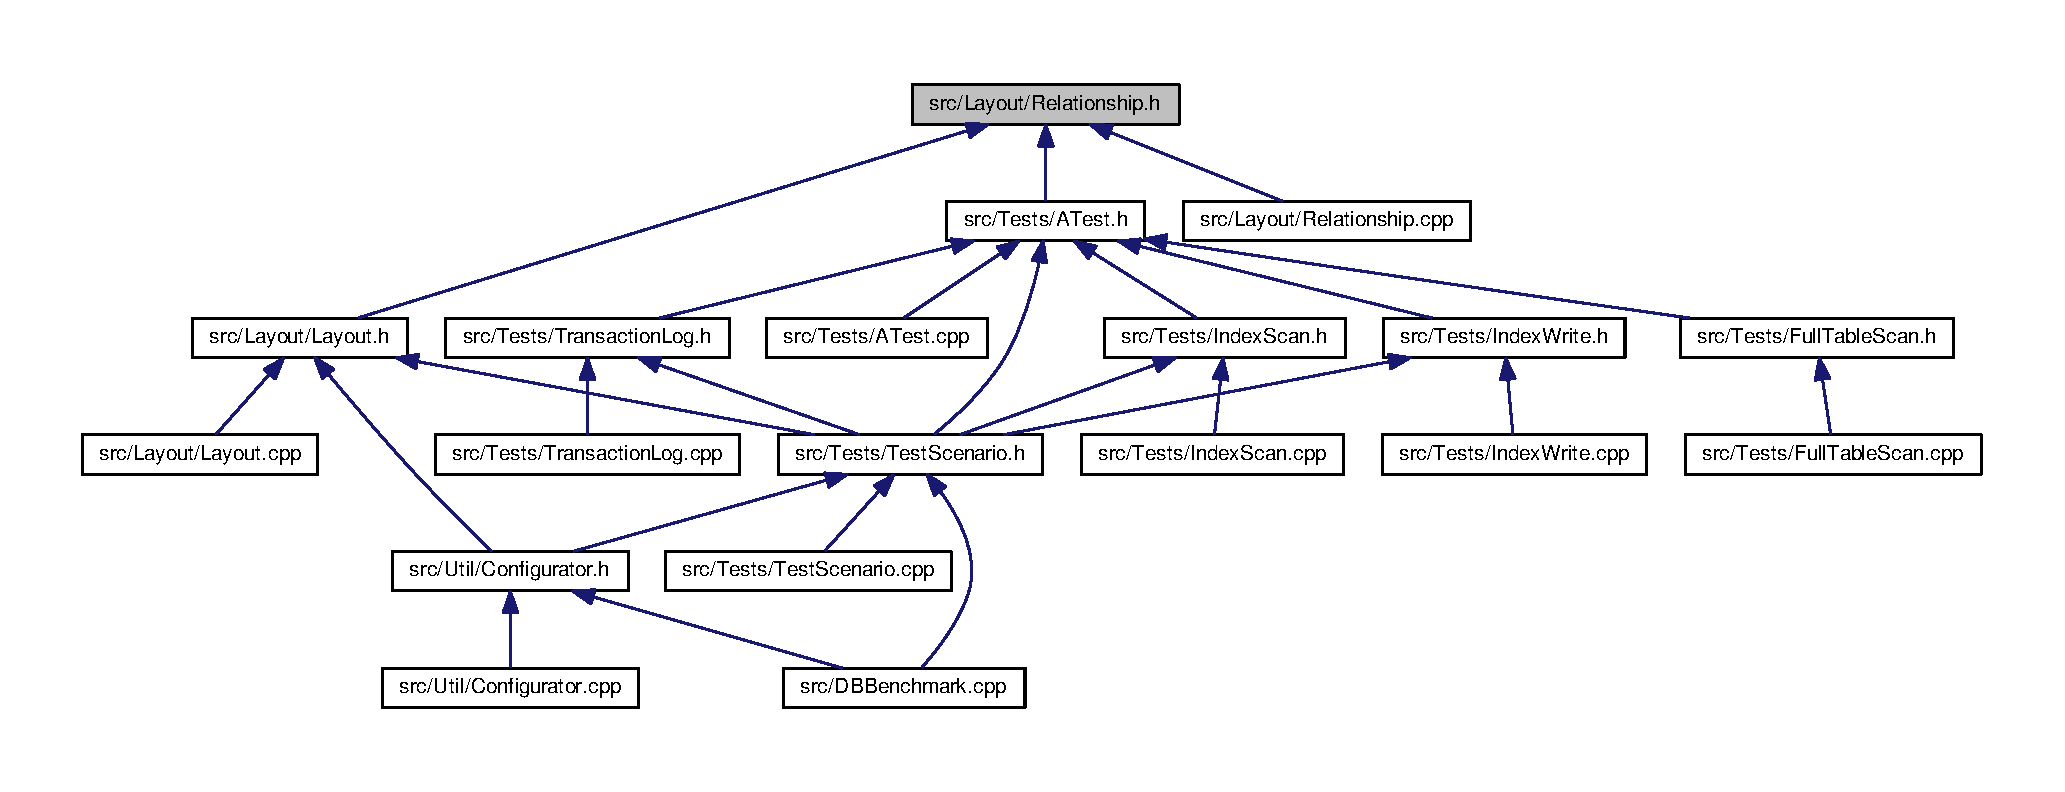
\includegraphics[width=350pt]{_relationship_8h__dep__incl}
\end{center}
\end{figure}
\subsection*{Classes}
\begin{DoxyCompactItemize}
\item 
struct \hyperlink{struct_h_d_d_test_1_1_extent}{H\-D\-D\-Test\-::\-Extent}
\item 
class \hyperlink{class_h_d_d_test_1_1_relationship}{H\-D\-D\-Test\-::\-Relationship}
\end{DoxyCompactItemize}
\subsection*{Namespaces}
\begin{DoxyCompactItemize}
\item 
\hyperlink{namespace_h_d_d_test}{H\-D\-D\-Test}
\end{DoxyCompactItemize}

\hypertarget{_a_test_8cpp}{\section{src/\-Tests/\-A\-Test.cpp File Reference}
\label{_a_test_8cpp}\index{src/\-Tests/\-A\-Test.\-cpp@{src/\-Tests/\-A\-Test.\-cpp}}
}
{\ttfamily \#include \char`\"{}A\-Test.\-h\char`\"{}}\\*
Include dependency graph for A\-Test.\-cpp\-:\nopagebreak
\begin{figure}[H]
\begin{center}
\leavevmode
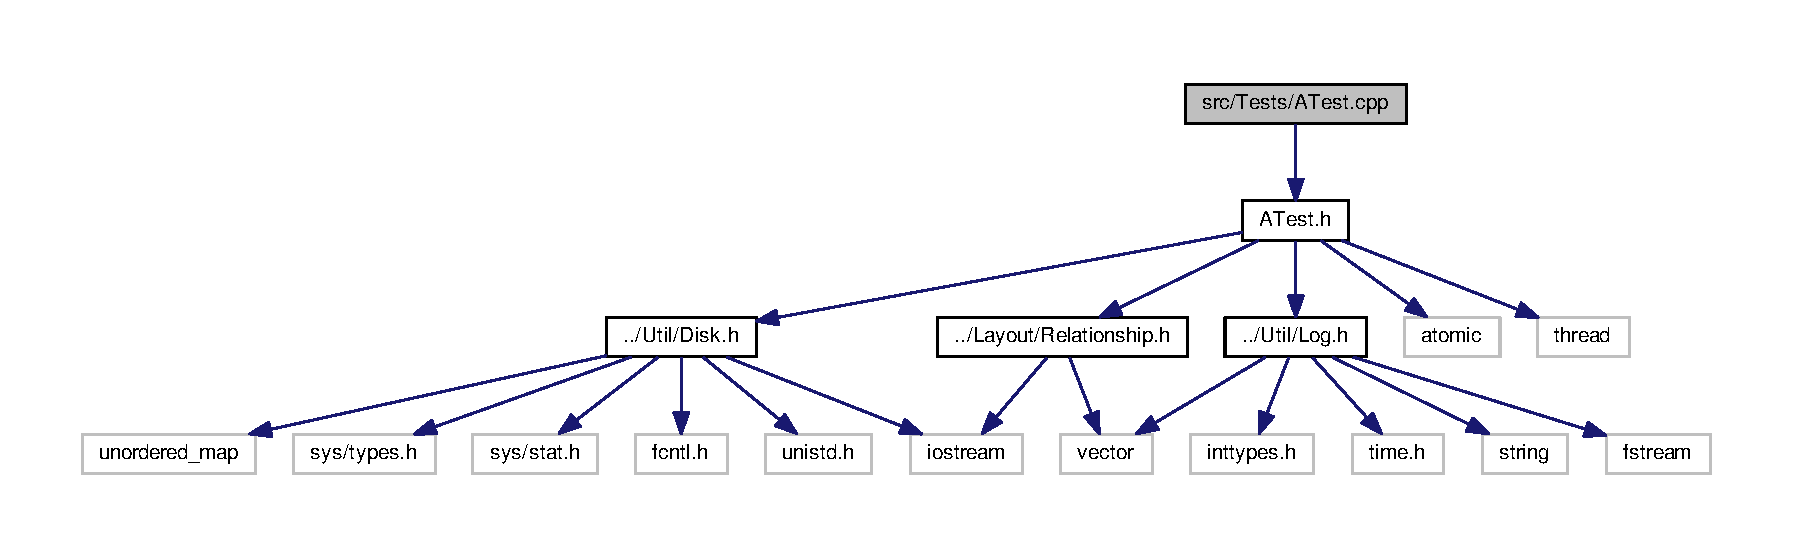
\includegraphics[width=350pt]{_a_test_8cpp__incl}
\end{center}
\end{figure}
\subsection*{Namespaces}
\begin{DoxyCompactItemize}
\item 
\hyperlink{namespace_h_d_d_test}{H\-D\-D\-Test}
\end{DoxyCompactItemize}

\hypertarget{_a_test_8h}{\section{src/\-Tests/\-A\-Test.h File Reference}
\label{_a_test_8h}\index{src/\-Tests/\-A\-Test.\-h@{src/\-Tests/\-A\-Test.\-h}}
}
{\ttfamily \#include \char`\"{}../\-Util/\-Disk.\-h\char`\"{}}\\*
{\ttfamily \#include \char`\"{}../\-Layout/\-Relationship.\-h\char`\"{}}\\*
{\ttfamily \#include \char`\"{}../\-Util/\-Log.\-h\char`\"{}}\\*
{\ttfamily \#include $<$atomic$>$}\\*
{\ttfamily \#include $<$thread$>$}\\*
{\ttfamily \#include $<$time.\-h$>$}\\*
Include dependency graph for A\-Test.\-h\-:
\nopagebreak
\begin{figure}[H]
\begin{center}
\leavevmode
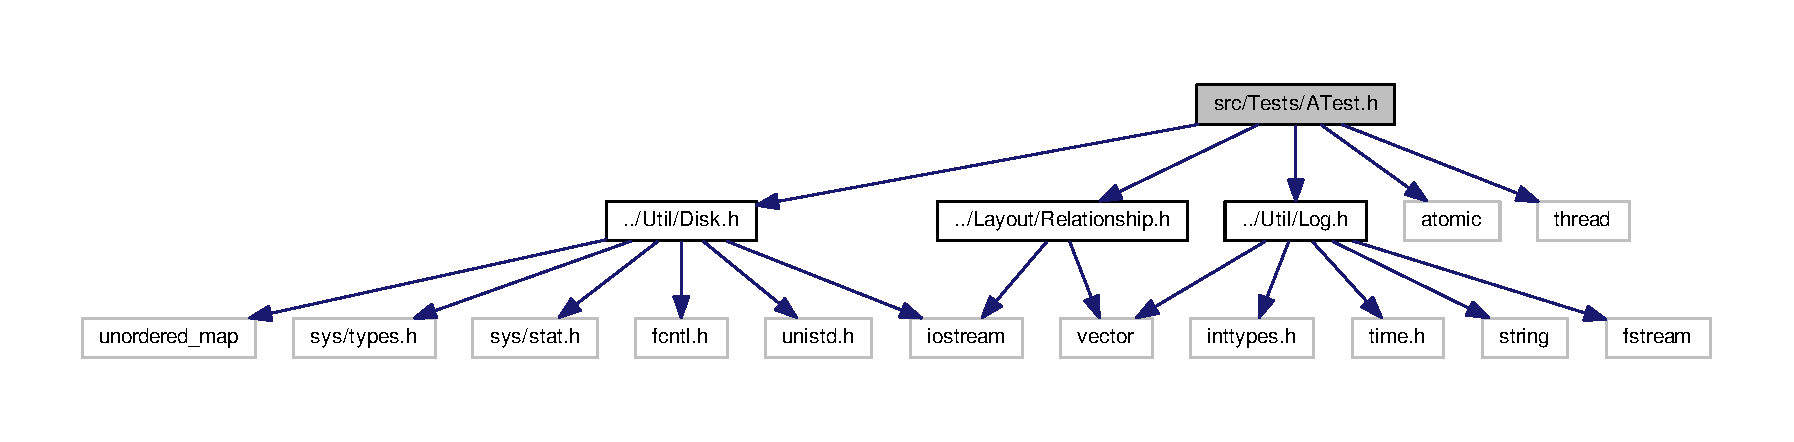
\includegraphics[width=350pt]{_a_test_8h__incl}
\end{center}
\end{figure}
This graph shows which files directly or indirectly include this file\-:
\nopagebreak
\begin{figure}[H]
\begin{center}
\leavevmode
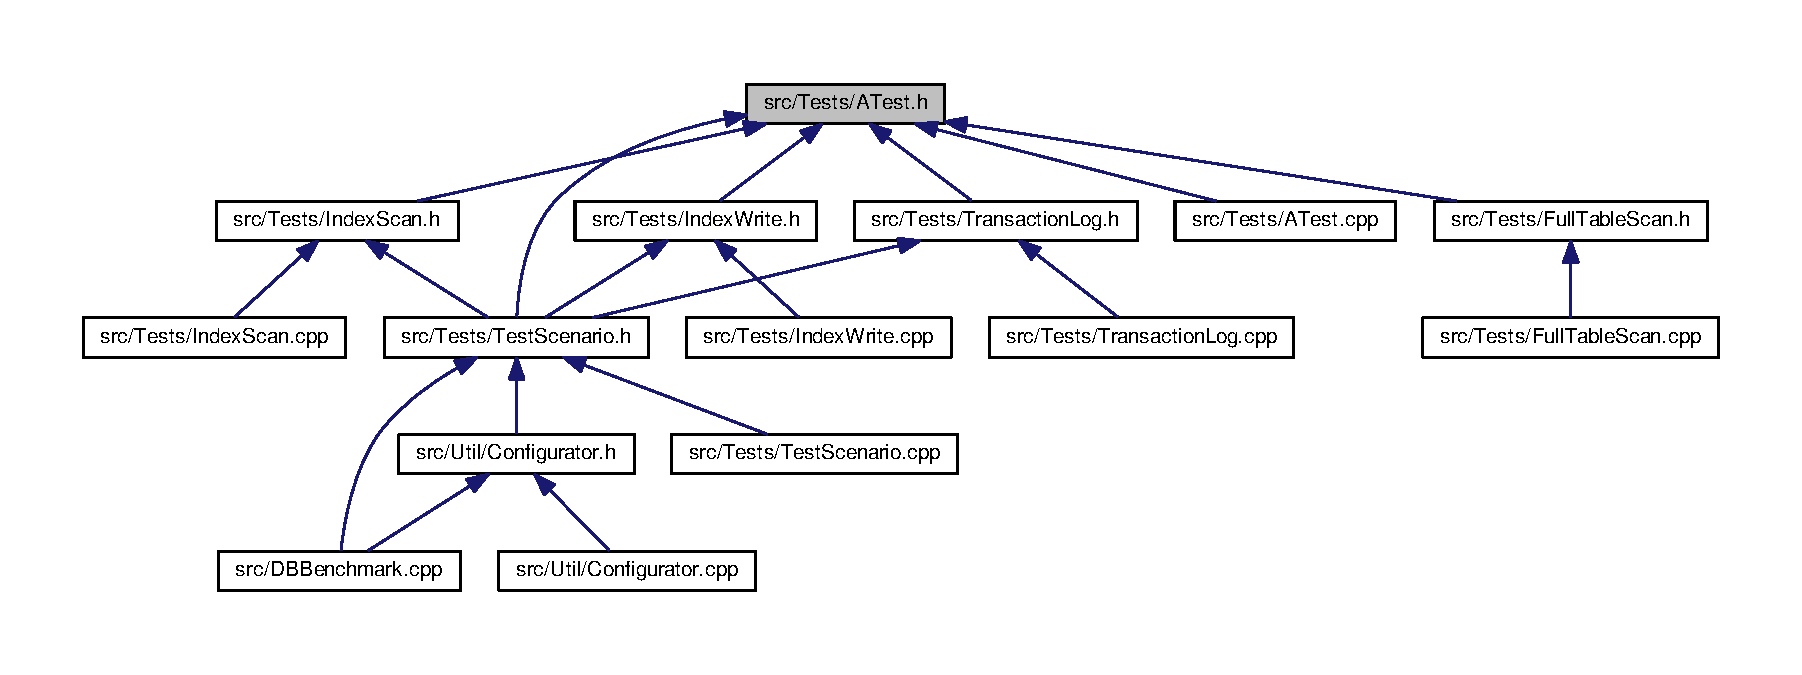
\includegraphics[width=350pt]{_a_test_8h__dep__incl}
\end{center}
\end{figure}
\subsection*{Classes}
\begin{DoxyCompactItemize}
\item 
struct \hyperlink{struct_h_d_d_test_1_1_test_settings}{H\-D\-D\-Test\-::\-Test\-Settings}
\item 
class \hyperlink{class_h_d_d_test_1_1_a_test}{H\-D\-D\-Test\-::\-A\-Test}
\end{DoxyCompactItemize}
\subsection*{Namespaces}
\begin{DoxyCompactItemize}
\item 
\hyperlink{namespace_h_d_d_test}{H\-D\-D\-Test}
\end{DoxyCompactItemize}

\hypertarget{_full_table_scan_8cpp}{\section{src/\-Tests/\-Full\-Table\-Scan.cpp File Reference}
\label{_full_table_scan_8cpp}\index{src/\-Tests/\-Full\-Table\-Scan.\-cpp@{src/\-Tests/\-Full\-Table\-Scan.\-cpp}}
}
{\ttfamily \#include \char`\"{}A\-Test.\-h\char`\"{}}\\*
Include dependency graph for Full\-Table\-Scan.\-cpp\-:
\nopagebreak
\begin{figure}[H]
\begin{center}
\leavevmode
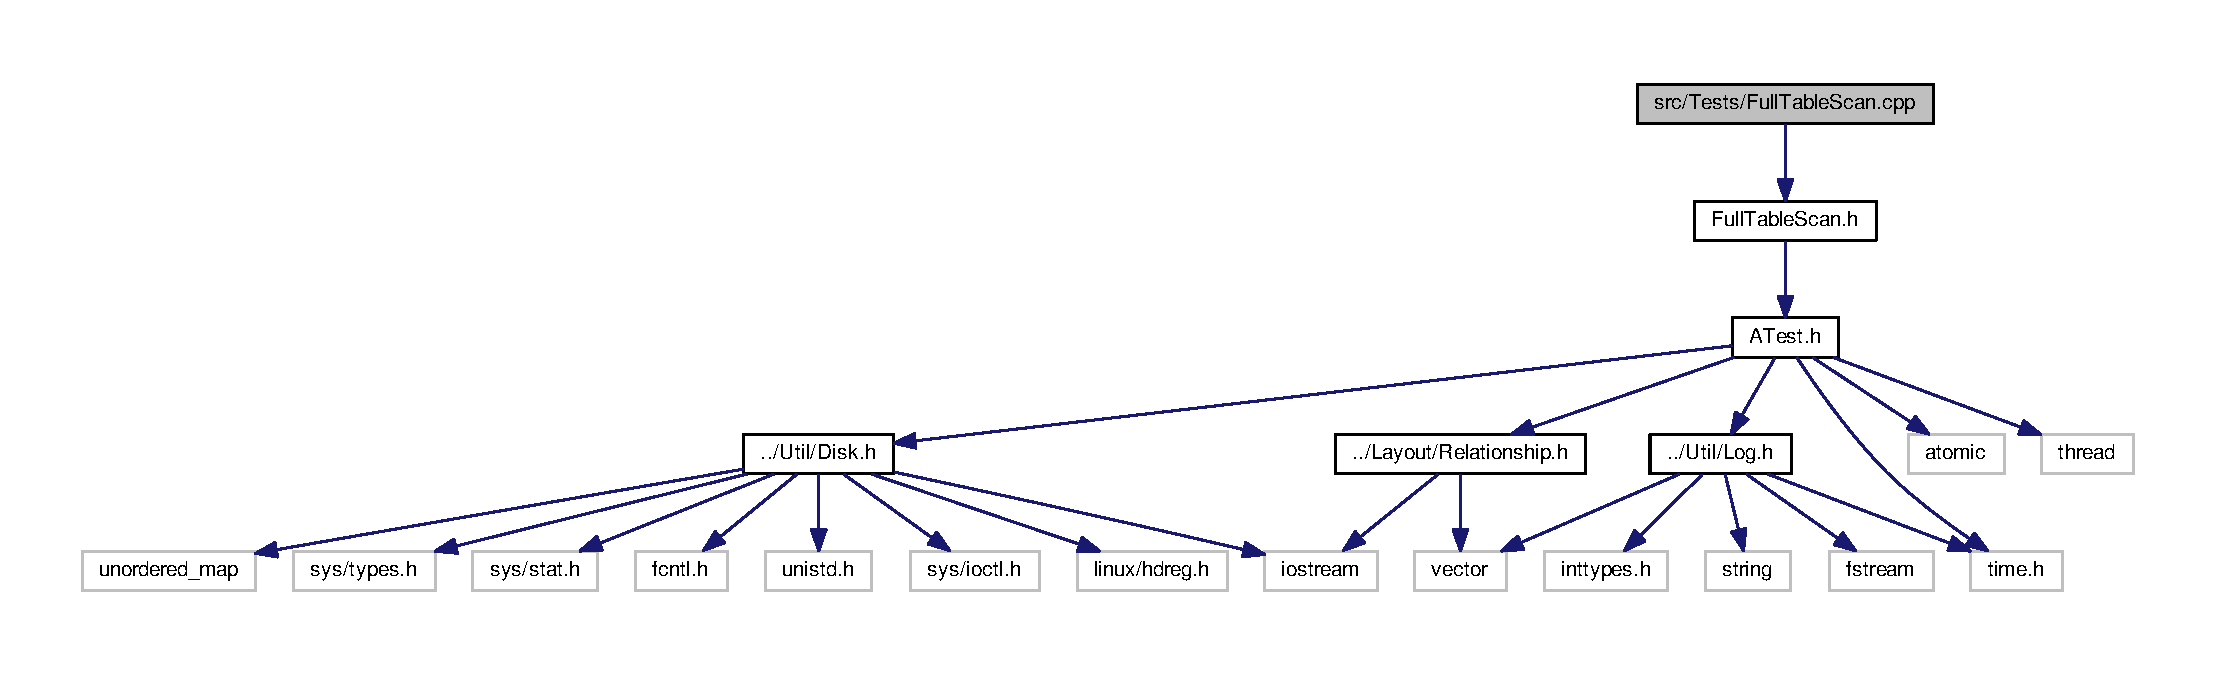
\includegraphics[width=350pt]{_full_table_scan_8cpp__incl}
\end{center}
\end{figure}
\subsection*{Classes}
\begin{DoxyCompactItemize}
\item 
class \hyperlink{class_h_d_d_test_1_1_full_table_scan}{H\-D\-D\-Test\-::\-Full\-Table\-Scan}
\end{DoxyCompactItemize}
\subsection*{Namespaces}
\begin{DoxyCompactItemize}
\item 
\hyperlink{namespace_h_d_d_test}{H\-D\-D\-Test}
\end{DoxyCompactItemize}
\subsection*{Macros}
\begin{DoxyCompactItemize}
\item 
\#define \hyperlink{_full_table_scan_8cpp_a1a05343cf317a02c2a82b5d4f731eb60}{S\-R\-C\-\_\-\-T\-E\-S\-T\-S\-\_\-\-F\-U\-L\-L\-T\-A\-B\-L\-E\-S\-C\-A\-N\-\_\-\-H\-\_\-}
\end{DoxyCompactItemize}


\subsection{Macro Definition Documentation}
\hypertarget{_full_table_scan_8cpp_a1a05343cf317a02c2a82b5d4f731eb60}{\index{Full\-Table\-Scan.\-cpp@{Full\-Table\-Scan.\-cpp}!S\-R\-C\-\_\-\-T\-E\-S\-T\-S\-\_\-\-F\-U\-L\-L\-T\-A\-B\-L\-E\-S\-C\-A\-N\-\_\-\-H\-\_\-@{S\-R\-C\-\_\-\-T\-E\-S\-T\-S\-\_\-\-F\-U\-L\-L\-T\-A\-B\-L\-E\-S\-C\-A\-N\-\_\-\-H\-\_\-}}
\index{S\-R\-C\-\_\-\-T\-E\-S\-T\-S\-\_\-\-F\-U\-L\-L\-T\-A\-B\-L\-E\-S\-C\-A\-N\-\_\-\-H\-\_\-@{S\-R\-C\-\_\-\-T\-E\-S\-T\-S\-\_\-\-F\-U\-L\-L\-T\-A\-B\-L\-E\-S\-C\-A\-N\-\_\-\-H\-\_\-}!FullTableScan.cpp@{Full\-Table\-Scan.\-cpp}}
\subsubsection[{S\-R\-C\-\_\-\-T\-E\-S\-T\-S\-\_\-\-F\-U\-L\-L\-T\-A\-B\-L\-E\-S\-C\-A\-N\-\_\-\-H\-\_\-}]{\setlength{\rightskip}{0pt plus 5cm}\#define S\-R\-C\-\_\-\-T\-E\-S\-T\-S\-\_\-\-F\-U\-L\-L\-T\-A\-B\-L\-E\-S\-C\-A\-N\-\_\-\-H\-\_\-}}\label{_full_table_scan_8cpp_a1a05343cf317a02c2a82b5d4f731eb60}


Definition at line 9 of file Full\-Table\-Scan.\-cpp.


\hypertarget{_full_table_scan_8h}{\section{src/\-Tests/\-Full\-Table\-Scan.h File Reference}
\label{_full_table_scan_8h}\index{src/\-Tests/\-Full\-Table\-Scan.\-h@{src/\-Tests/\-Full\-Table\-Scan.\-h}}
}
{\ttfamily \#include \char`\"{}Full\-Table\-Scan.\-h\char`\"{}}\\*
Include dependency graph for Full\-Table\-Scan.\-h\-:
\nopagebreak
\begin{figure}[H]
\begin{center}
\leavevmode
\includegraphics[width=228pt]{_full_table_scan_8h__incl}
\end{center}
\end{figure}
This graph shows which files directly or indirectly include this file\-:
\nopagebreak
\begin{figure}[H]
\begin{center}
\leavevmode
\includegraphics[width=228pt]{_full_table_scan_8h__dep__incl}
\end{center}
\end{figure}
\subsection*{Namespaces}
\begin{DoxyCompactItemize}
\item 
\hyperlink{namespace_h_d_d_test}{H\-D\-D\-Test}
\end{DoxyCompactItemize}

\hypertarget{_index_scan_8cpp}{\section{src/\-Tests/\-Index\-Scan.cpp File Reference}
\label{_index_scan_8cpp}\index{src/\-Tests/\-Index\-Scan.\-cpp@{src/\-Tests/\-Index\-Scan.\-cpp}}
}
{\ttfamily \#include \char`\"{}Index\-Scan.\-h\char`\"{}}\\*
{\ttfamily \#include \char`\"{}../\-Util/\-Progressbar.\-h\char`\"{}}\\*
Include dependency graph for Index\-Scan.\-cpp\-:
\nopagebreak
\begin{figure}[H]
\begin{center}
\leavevmode
\includegraphics[width=350pt]{_index_scan_8cpp__incl}
\end{center}
\end{figure}
\subsection*{Namespaces}
\begin{DoxyCompactItemize}
\item 
\hyperlink{namespace_h_d_d_test}{H\-D\-D\-Test}
\end{DoxyCompactItemize}

\hypertarget{_index_scan_8h}{\section{src/\-Tests/\-Index\-Scan.h File Reference}
\label{_index_scan_8h}\index{src/\-Tests/\-Index\-Scan.\-h@{src/\-Tests/\-Index\-Scan.\-h}}
}
{\ttfamily \#include \char`\"{}A\-Test.\-h\char`\"{}}\\*
Include dependency graph for Index\-Scan.\-h\-:
\nopagebreak
\begin{figure}[H]
\begin{center}
\leavevmode
\includegraphics[width=350pt]{_index_scan_8h__incl}
\end{center}
\end{figure}
This graph shows which files directly or indirectly include this file\-:\nopagebreak
\begin{figure}[H]
\begin{center}
\leavevmode
\includegraphics[width=350pt]{_index_scan_8h__dep__incl}
\end{center}
\end{figure}
\subsection*{Classes}
\begin{DoxyCompactItemize}
\item 
class \hyperlink{class_h_d_d_test_1_1_index_scan}{H\-D\-D\-Test\-::\-Index\-Scan}
\end{DoxyCompactItemize}
\subsection*{Namespaces}
\begin{DoxyCompactItemize}
\item 
\hyperlink{namespace_h_d_d_test}{H\-D\-D\-Test}
\end{DoxyCompactItemize}

\hypertarget{_index_write_8cpp}{\section{src/\-Tests/\-Index\-Write.cpp File Reference}
\label{_index_write_8cpp}\index{src/\-Tests/\-Index\-Write.\-cpp@{src/\-Tests/\-Index\-Write.\-cpp}}
}
{\ttfamily \#include \char`\"{}Index\-Write.\-h\char`\"{}}\\*
{\ttfamily \#include \char`\"{}../\-Util/\-Progressbar.\-h\char`\"{}}\\*
Include dependency graph for Index\-Write.\-cpp\-:
\nopagebreak
\begin{figure}[H]
\begin{center}
\leavevmode
\includegraphics[width=350pt]{_index_write_8cpp__incl}
\end{center}
\end{figure}
\subsection*{Namespaces}
\begin{DoxyCompactItemize}
\item 
\hyperlink{namespace_h_d_d_test}{H\-D\-D\-Test}
\end{DoxyCompactItemize}

\hypertarget{_index_write_8h}{\section{src/\-Tests/\-Index\-Write.h File Reference}
\label{_index_write_8h}\index{src/\-Tests/\-Index\-Write.\-h@{src/\-Tests/\-Index\-Write.\-h}}
}
{\ttfamily \#include \char`\"{}A\-Test.\-h\char`\"{}}\\*
Include dependency graph for Index\-Write.\-h\-:
\nopagebreak
\begin{figure}[H]
\begin{center}
\leavevmode
\includegraphics[width=350pt]{_index_write_8h__incl}
\end{center}
\end{figure}
This graph shows which files directly or indirectly include this file\-:
\nopagebreak
\begin{figure}[H]
\begin{center}
\leavevmode
\includegraphics[width=350pt]{_index_write_8h__dep__incl}
\end{center}
\end{figure}
\subsection*{Classes}
\begin{DoxyCompactItemize}
\item 
class \hyperlink{class_h_d_d_test_1_1_index_write}{H\-D\-D\-Test\-::\-Index\-Write}
\end{DoxyCompactItemize}
\subsection*{Namespaces}
\begin{DoxyCompactItemize}
\item 
\hyperlink{namespace_h_d_d_test}{H\-D\-D\-Test}
\end{DoxyCompactItemize}

\hypertarget{_test_scenario_8cpp}{\section{src/\-Tests/\-Test\-Scenario.cpp File Reference}
\label{_test_scenario_8cpp}\index{src/\-Tests/\-Test\-Scenario.\-cpp@{src/\-Tests/\-Test\-Scenario.\-cpp}}
}
{\ttfamily \#include \char`\"{}Test\-Scenario.\-h\char`\"{}}\\*
{\ttfamily \#include \char`\"{}../\-Util/\-Progressbar.\-h\char`\"{}}\\*
Include dependency graph for Test\-Scenario.\-cpp\-:\nopagebreak
\begin{figure}[H]
\begin{center}
\leavevmode
\includegraphics[width=350pt]{_test_scenario_8cpp__incl}
\end{center}
\end{figure}
\subsection*{Namespaces}
\begin{DoxyCompactItemize}
\item 
\hyperlink{namespace_h_d_d_test}{H\-D\-D\-Test}
\end{DoxyCompactItemize}

\hypertarget{_test_scenario_8h}{\section{src/\-Tests/\-Test\-Scenario.h File Reference}
\label{_test_scenario_8h}\index{src/\-Tests/\-Test\-Scenario.\-h@{src/\-Tests/\-Test\-Scenario.\-h}}
}
{\ttfamily \#include $<$vector$>$}\\*
{\ttfamily \#include \char`\"{}../\-Layout/\-Layout.\-h\char`\"{}}\\*
{\ttfamily \#include \char`\"{}../\-Util/\-Disk.\-h\char`\"{}}\\*
{\ttfamily \#include \char`\"{}A\-Test.\-h\char`\"{}}\\*
{\ttfamily \#include \char`\"{}Index\-Scan.\-h\char`\"{}}\\*
Include dependency graph for Test\-Scenario.\-h\-:\nopagebreak
\begin{figure}[H]
\begin{center}
\leavevmode
\includegraphics[width=350pt]{_test_scenario_8h__incl}
\end{center}
\end{figure}
This graph shows which files directly or indirectly include this file\-:\nopagebreak
\begin{figure}[H]
\begin{center}
\leavevmode
\includegraphics[width=350pt]{_test_scenario_8h__dep__incl}
\end{center}
\end{figure}
\subsection*{Classes}
\begin{DoxyCompactItemize}
\item 
class \hyperlink{class_h_d_d_test_1_1_test_scenario}{H\-D\-D\-Test\-::\-Test\-Scenario}
\end{DoxyCompactItemize}
\subsection*{Namespaces}
\begin{DoxyCompactItemize}
\item 
\hyperlink{namespace_h_d_d_test}{H\-D\-D\-Test}
\end{DoxyCompactItemize}

\hypertarget{_transaction_log_8cpp}{\section{src/\-Tests/\-Transaction\-Log.cpp File Reference}
\label{_transaction_log_8cpp}\index{src/\-Tests/\-Transaction\-Log.\-cpp@{src/\-Tests/\-Transaction\-Log.\-cpp}}
}
{\ttfamily \#include \char`\"{}Transaction\-Log.\-h\char`\"{}}\\*
Include dependency graph for Transaction\-Log.\-cpp\-:
\nopagebreak
\begin{figure}[H]
\begin{center}
\leavevmode
\includegraphics[width=350pt]{_transaction_log_8cpp__incl}
\end{center}
\end{figure}
\subsection*{Namespaces}
\begin{DoxyCompactItemize}
\item 
\hyperlink{namespace_h_d_d_test}{H\-D\-D\-Test}
\end{DoxyCompactItemize}

\hypertarget{_transaction_log_8h}{\section{src/\-Tests/\-Transaction\-Log.h File Reference}
\label{_transaction_log_8h}\index{src/\-Tests/\-Transaction\-Log.\-h@{src/\-Tests/\-Transaction\-Log.\-h}}
}
{\ttfamily \#include \char`\"{}A\-Test.\-h\char`\"{}}\\*
Include dependency graph for Transaction\-Log.\-h\-:
\nopagebreak
\begin{figure}[H]
\begin{center}
\leavevmode
\includegraphics[width=350pt]{_transaction_log_8h__incl}
\end{center}
\end{figure}
This graph shows which files directly or indirectly include this file\-:
\nopagebreak
\begin{figure}[H]
\begin{center}
\leavevmode
\includegraphics[width=350pt]{_transaction_log_8h__dep__incl}
\end{center}
\end{figure}
\subsection*{Classes}
\begin{DoxyCompactItemize}
\item 
class \hyperlink{class_h_d_d_test_1_1_transaction_log}{H\-D\-D\-Test\-::\-Transaction\-Log}
\end{DoxyCompactItemize}
\subsection*{Namespaces}
\begin{DoxyCompactItemize}
\item 
\hyperlink{namespace_h_d_d_test}{H\-D\-D\-Test}
\end{DoxyCompactItemize}

\hypertarget{_configurator_8cpp}{\section{src/\-Util/\-Configurator.cpp File Reference}
\label{_configurator_8cpp}\index{src/\-Util/\-Configurator.\-cpp@{src/\-Util/\-Configurator.\-cpp}}
}
{\ttfamily \#include \char`\"{}Configurator.\-h\char`\"{}}\\*
Include dependency graph for Configurator.\-cpp\-:
\nopagebreak
\begin{figure}[H]
\begin{center}
\leavevmode
\includegraphics[width=350pt]{_configurator_8cpp__incl}
\end{center}
\end{figure}
\subsection*{Namespaces}
\begin{DoxyCompactItemize}
\item 
\hyperlink{namespace_h_d_d_test}{H\-D\-D\-Test}
\end{DoxyCompactItemize}

\hypertarget{_configurator_8h}{\section{src/\-Util/\-Configurator.h File Reference}
\label{_configurator_8h}\index{src/\-Util/\-Configurator.\-h@{src/\-Util/\-Configurator.\-h}}
}
{\ttfamily \#include $<$rapidjson/document.\-h$>$}\\*
{\ttfamily \#include $<$rapidjson/filestream.\-h$>$}\\*
{\ttfamily \#include $<$iostream$>$}\\*
{\ttfamily \#include $<$unistd.\-h$>$}\\*
{\ttfamily \#include $<$vector$>$}\\*
{\ttfamily \#include $<$unordered\-\_\-map$>$}\\*
{\ttfamily \#include \char`\"{}../\-Tests/\-Test\-Scenario.\-h\char`\"{}}\\*
{\ttfamily \#include \char`\"{}Disk.\-h\char`\"{}}\\*
{\ttfamily \#include \char`\"{}../\-Layout/\-Layout.\-h\char`\"{}}\\*
Include dependency graph for Configurator.\-h\-:\nopagebreak
\begin{figure}[H]
\begin{center}
\leavevmode
\includegraphics[width=350pt]{_configurator_8h__incl}
\end{center}
\end{figure}
This graph shows which files directly or indirectly include this file\-:\nopagebreak
\begin{figure}[H]
\begin{center}
\leavevmode
\includegraphics[width=337pt]{_configurator_8h__dep__incl}
\end{center}
\end{figure}
\subsection*{Classes}
\begin{DoxyCompactItemize}
\item 
class \hyperlink{class_h_d_d_test_1_1_configurator}{H\-D\-D\-Test\-::\-Configurator}
\end{DoxyCompactItemize}
\subsection*{Namespaces}
\begin{DoxyCompactItemize}
\item 
\hyperlink{namespace_h_d_d_test}{H\-D\-D\-Test}
\end{DoxyCompactItemize}

\hypertarget{_disk_8cpp}{\section{src/\-Util/\-Disk.cpp File Reference}
\label{_disk_8cpp}\index{src/\-Util/\-Disk.\-cpp@{src/\-Util/\-Disk.\-cpp}}
}
{\ttfamily \#include \char`\"{}Disk.\-h\char`\"{}}\\*
Include dependency graph for Disk.\-cpp\-:
\nopagebreak
\begin{figure}[H]
\begin{center}
\leavevmode
\includegraphics[width=350pt]{_disk_8cpp__incl}
\end{center}
\end{figure}
\subsection*{Namespaces}
\begin{DoxyCompactItemize}
\item 
\hyperlink{namespace_h_d_d_test}{H\-D\-D\-Test}
\end{DoxyCompactItemize}

\hypertarget{_disk_8h}{\section{src/\-Util/\-Disk.h File Reference}
\label{_disk_8h}\index{src/\-Util/\-Disk.\-h@{src/\-Util/\-Disk.\-h}}
}
{\ttfamily \#include $<$unordered\-\_\-map$>$}\\*
{\ttfamily \#include $<$sys/types.\-h$>$}\\*
{\ttfamily \#include $<$sys/stat.\-h$>$}\\*
{\ttfamily \#include $<$fcntl.\-h$>$}\\*
{\ttfamily \#include $<$unistd.\-h$>$}\\*
{\ttfamily \#include $<$iostream$>$}\\*
{\ttfamily \#include $<$sys/ioctl.\-h$>$}\\*
{\ttfamily \#include $<$linux/hdreg.\-h$>$}\\*
Include dependency graph for Disk.\-h\-:
\nopagebreak
\begin{figure}[H]
\begin{center}
\leavevmode
\includegraphics[width=350pt]{_disk_8h__incl}
\end{center}
\end{figure}
This graph shows which files directly or indirectly include this file\-:
\nopagebreak
\begin{figure}[H]
\begin{center}
\leavevmode
\includegraphics[width=350pt]{_disk_8h__dep__incl}
\end{center}
\end{figure}
\subsection*{Classes}
\begin{DoxyCompactItemize}
\item 
class \hyperlink{class_h_d_d_test_1_1_disk}{H\-D\-D\-Test\-::\-Disk}
\end{DoxyCompactItemize}
\subsection*{Namespaces}
\begin{DoxyCompactItemize}
\item 
\hyperlink{namespace_h_d_d_test}{H\-D\-D\-Test}
\end{DoxyCompactItemize}

\hypertarget{_log_8cpp}{\section{src/\-Util/\-Log.cpp File Reference}
\label{_log_8cpp}\index{src/\-Util/\-Log.\-cpp@{src/\-Util/\-Log.\-cpp}}
}
{\ttfamily \#include \char`\"{}Log.\-h\char`\"{}}\\*
{\ttfamily \#include \char`\"{}rapidjson/writer.\-h\char`\"{}}\\*
{\ttfamily \#include \char`\"{}rapidjson/stringbuffer.\-h\char`\"{}}\\*
Include dependency graph for Log.\-cpp\-:\nopagebreak
\begin{figure}[H]
\begin{center}
\leavevmode
\includegraphics[width=350pt]{_log_8cpp__incl}
\end{center}
\end{figure}
\subsection*{Namespaces}
\begin{DoxyCompactItemize}
\item 
\hyperlink{namespace_d_b_util}{D\-B\-Util}
\end{DoxyCompactItemize}

\hypertarget{_log_8h}{\section{src/\-Util/\-Log.h File Reference}
\label{_log_8h}\index{src/\-Util/\-Log.\-h@{src/\-Util/\-Log.\-h}}
}
{\ttfamily \#include $<$inttypes.\-h$>$}\\*
{\ttfamily \#include $<$time.\-h$>$}\\*
{\ttfamily \#include $<$vector$>$}\\*
{\ttfamily \#include $<$string$>$}\\*
{\ttfamily \#include $<$fstream$>$}\\*
Include dependency graph for Log.\-h\-:
\nopagebreak
\begin{figure}[H]
\begin{center}
\leavevmode
\includegraphics[width=350pt]{_log_8h__incl}
\end{center}
\end{figure}
This graph shows which files directly or indirectly include this file\-:
\nopagebreak
\begin{figure}[H]
\begin{center}
\leavevmode
\includegraphics[width=350pt]{_log_8h__dep__incl}
\end{center}
\end{figure}
\subsection*{Classes}
\begin{DoxyCompactItemize}
\item 
struct \hyperlink{struct_d_b_util_1_1measurement}{D\-B\-Util\-::measurement}
\item 
class \hyperlink{class_d_b_util_1_1_log}{D\-B\-Util\-::\-Log}
\end{DoxyCompactItemize}
\subsection*{Namespaces}
\begin{DoxyCompactItemize}
\item 
\hyperlink{namespace_d_b_util}{D\-B\-Util}
\end{DoxyCompactItemize}

\hypertarget{_progressbar_8cpp}{\section{src/\-Util/\-Progressbar.cpp File Reference}
\label{_progressbar_8cpp}\index{src/\-Util/\-Progressbar.\-cpp@{src/\-Util/\-Progressbar.\-cpp}}
}
{\ttfamily \#include \char`\"{}Progressbar.\-h\char`\"{}}\\*
Include dependency graph for Progressbar.\-cpp\-:
\nopagebreak
\begin{figure}[H]
\begin{center}
\leavevmode
\includegraphics[width=203pt]{_progressbar_8cpp__incl}
\end{center}
\end{figure}
\subsection*{Namespaces}
\begin{DoxyCompactItemize}
\item 
\hyperlink{namespace_h_d_d_test}{H\-D\-D\-Test}
\end{DoxyCompactItemize}

\hypertarget{_progressbar_8h}{\section{src/\-Util/\-Progressbar.h File Reference}
\label{_progressbar_8h}\index{src/\-Util/\-Progressbar.\-h@{src/\-Util/\-Progressbar.\-h}}
}
{\ttfamily \#include $<$stdint.\-h$>$}\\*
{\ttfamily \#include $<$iostream$>$}\\*
Include dependency graph for Progressbar.\-h\-:\nopagebreak
\begin{figure}[H]
\begin{center}
\leavevmode
\includegraphics[width=201pt]{_progressbar_8h__incl}
\end{center}
\end{figure}
This graph shows which files directly or indirectly include this file\-:
\nopagebreak
\begin{figure}[H]
\begin{center}
\leavevmode
\includegraphics[width=350pt]{_progressbar_8h__dep__incl}
\end{center}
\end{figure}
\subsection*{Classes}
\begin{DoxyCompactItemize}
\item 
class \hyperlink{class_h_d_d_test_1_1_progressbar}{H\-D\-D\-Test\-::\-Progressbar}
\end{DoxyCompactItemize}
\subsection*{Namespaces}
\begin{DoxyCompactItemize}
\item 
\hyperlink{namespace_h_d_d_test}{H\-D\-D\-Test}
\end{DoxyCompactItemize}

\hypertarget{_randomizer_8cpp}{\section{src/\-Util/\-Randomizer.cpp File Reference}
\label{_randomizer_8cpp}\index{src/\-Util/\-Randomizer.\-cpp@{src/\-Util/\-Randomizer.\-cpp}}
}
{\ttfamily \#include \char`\"{}Randomizer.\-h\char`\"{}}\\*
Include dependency graph for Randomizer.\-cpp\-:
\nopagebreak
\begin{figure}[H]
\begin{center}
\leavevmode
\includegraphics[width=202pt]{_randomizer_8cpp__incl}
\end{center}
\end{figure}
\subsection*{Namespaces}
\begin{DoxyCompactItemize}
\item 
\hyperlink{namespace_h_d_d_test}{H\-D\-D\-Test}
\end{DoxyCompactItemize}

\hypertarget{_randomizer_8h}{\section{src/\-Util/\-Randomizer.h File Reference}
\label{_randomizer_8h}\index{src/\-Util/\-Randomizer.\-h@{src/\-Util/\-Randomizer.\-h}}
}
{\ttfamily \#include $<$random$>$}\\*
Include dependency graph for Randomizer.\-h\-:
\nopagebreak
\begin{figure}[H]
\begin{center}
\leavevmode
\includegraphics[width=190pt]{_randomizer_8h__incl}
\end{center}
\end{figure}
This graph shows which files directly or indirectly include this file\-:
\nopagebreak
\begin{figure}[H]
\begin{center}
\leavevmode
\includegraphics[width=202pt]{_randomizer_8h__dep__incl}
\end{center}
\end{figure}
\subsection*{Classes}
\begin{DoxyCompactItemize}
\item 
class \hyperlink{class_h_d_d_test_1_1_randomizer}{H\-D\-D\-Test\-::\-Randomizer}
\end{DoxyCompactItemize}
\subsection*{Namespaces}
\begin{DoxyCompactItemize}
\item 
\hyperlink{namespace_h_d_d_test}{H\-D\-D\-Test}
\end{DoxyCompactItemize}

%--- End generated contents ---

% Index
\newpage
\phantomsection
\addcontentsline{toc}{chapter}{Index}
\printindex

\end{document}
